\documentclass[a4paper, 11pt, oneside]{thesis}

\usepackage[utf8]{inputenc}
\usepackage[T1]{fontenc}
\usepackage{lmodern}

\usepackage[square, numbers, comma, sort&compress]{natbib}

\usepackage{changepage}
\usepackage{float}
\usepackage[section]{placeins}

\usepackage{xcolor} 
\definecolor{rred}{HTML}{e0304e}

\lstset{
  captionpos=b,
  frame=tb,
  comment=[l]{\#},
  basicstyle=\ttfamily\footnotesize\linespread{1.2}\selectfont,
  numberstyle=\footnotesize\color{gray},
  commentstyle=\itshape,
  showstringspaces=false,
  keepspaces=true,
  aboveskip=2em,
  numbers=left,
  escapeinside={<@}{@>},
  moredelim=**[is][\color{rred}]{[@}{@]}
}

\usepackage[capitalise,noabbrev]{cleveref}
\crefname{sublstlisting}{Listing}{Listings}
\Crefname{sublstlisting}{Listing}{Listings}
\crefdefaultlabelformat{#2{\scshape #1}#3}
\AtBeginDocument{\DeclareCaptionSubType{lstlisting}}

\usepackage{varwidth}
\usepackage{verbatim}
\usepackage{stmaryrd}
\usepackage{mathtools}
\DeclarePairedDelimiter\set{\lbrace}{\rbrace}
\DeclarePairedDelimiter\bbrackets{\llbracket}{\rrbracket}
\DeclarePairedDelimiter\angles{\langle}{\rangle}
\DeclarePairedDelimiter\ttangles{\mathtt{<}}{\mathtt{>}}
\newcommand{\univ}{\ensuremath{\mathbb{U}}}

\usepackage{bussproofs}
\def\labelSpacing{1em}
\usepackage[altpo,epsilon]{backnaur}
\newcommand{\bnfmor}[1]{\bnfmore{\hspace{-1.5em}\ooalign{|\cr\hspace{1.5em}}#1}}

\usepackage{tipa}
\newcommand{\ipa}[1]{{\usefont{T3}{cmr}{m}{n}\selectfont#1}}

\usepackage{tikz}
\usetikzlibrary{chains,shapes,arrows,calc,positioning}
\tikzstyle{arrow} = [draw, -latex']
\tikzstyle{box} = [rectangle, draw=black!50, align=left, font={\ttfamily}]
\tikzstyle{init} = [circle, draw=black!50]
\tikzstyle{circ} = [circle, font={\ttfamily}]

\usepackage{siunitx}
\usepackage{csvsimple}
\usepackage{pgfplots}
\pgfplotsset{compat=1.18}
\usepackage{pgfplotstable}
\usepackage{xstring}
\pgfplotsset{where/.style 2 args={
    x filter/.code={
      \IfStrEq{\thisrow{#1}}{#2}{}{\def\pgfmathresult{}}
    }
  }
}

\graphicspath{{figures/}}
\def\datapath{data}

\begin{document}

\frontmatter

%TC:ignore
\university{{The University of Melbourne}}
\UNIVERSITY{{THE UNIVERSITY OF MELBOURNE}}
\department{{Department of Computing and Information Systems}}
\school{{Melbourne School of Engineering and IT}}
\degree{{Master of Computer Science}}
\title{{Higher-Order Programming in Wybe}}
\shortauthors{{James Barnes}}
\authors{
  \texorpdfstring{\href{mailto:barnesj2@student.unimelb.edu.au}{\shortauthornames}}{\shortauthornames}\\
  \small Student Number: 820946
}
\supervisor{{Dr.~Peter Schachte}}
\addresses{\deptname\\\univname}
\date{June 2022}
\subject{}
\keywords{}
%TC:endignore

%TC:envir lstlisting [option:text] xall
%TC:ignore
\wordcount{\input{|"bash ./scripts/fmt-texcount.sh \jobname.tex"}}
%TC:endignore

\maketitle

\setstretch{1.3}

\fancyhead{}
\rhead{\thepage}
\lhead{}

\pagestyle{fancy}

%TC:ignore
\quotepage{
  The lurking suspicion that something could \\
  be simplified is the world's richest source \\
  of rewarding challenges.
}{
  Edsger \textit{Wybe} Dijkstra
}

%TC:ignore

\addtotoc{Abstract}  
\abstract{
\addtocontents{toc}{\vspace{1em}} 

Higher-order programming allows for a greater level of abstraction over first-order programming. Allowing for procedures to be passed into or out of a procedure is the hallmark of this programming style. An emerging programming language, Wybe, currently does not support higher order programming, nor does the intermediate representation used internally by the Wybe compiler, logic programming virtual machine (LPVM). In this research, we propose an extension to LPVM, and further to Wybe, to support higher order programming. Wybe presents novel language features, which together with higher order programming, provide a novel language implementation space.

}

%TC:endignore

\Declaration{
  I, \shortauthornames, declare that this thesis and the work presented in it are my own. I confirm that:

  \begin{itemize}
    \item[\tiny{$\blacksquare$}] this thesis does not incorporate without acknowledgement any material previously submitted for a degree or diploma in any university; and that to the best of my knowledge and belief it does not contain any material previously published or written by another person where due reference is not made in the text.

    \item[\tiny{$\blacksquare$}] this thesis did not require clearance from the University's ethics committee.
    
    \item[\tiny{$\blacksquare$}] the thesis is approximately \totalwordcount words in length (excluding text in figures, tables, code listings, bibliographies, and appendices).
  \end{itemize}
}{\raisebox{-1.5em}{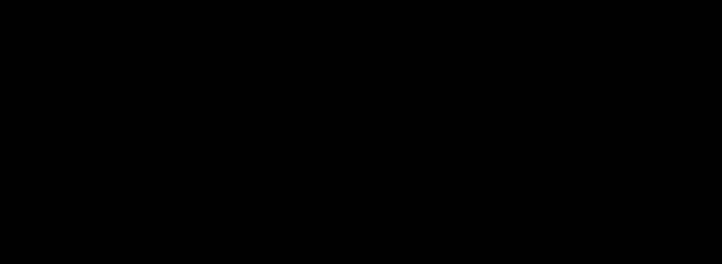
\includegraphics[width=0.25\textwidth]{sig.pdf}}}

\clearpage

\Preface{
  This thesis focuses on an established language, Wybe, that existed before the commencement of this piece of work. All code written by myself in support of this piece of work was independently reviewed by my supervisor, \supname. Feedback received was then further incorporated into the code. Any previously existing code is documented as being such throughout this document. Feedback was also received from my supervisor throughout the creation of this thesis and was incorporated into the final product.

  The literature review portion of this thesis is taken from, and further modified from, the research proposal that was undertaken to fulfill another portion of the requirements of the \degreename. This literature review was ultimately inspired by the work of myself in the completion of COMP90044 (Research Methods), prior.
}

\clearpage

\acknowledgements{
  I would like to acknowledge the people of the Kulin nations, the traditional custodians of the lands on which this work was produced, particularly the Wurundjeri and Wathaurong people, whose lands I both work on and reside in. I pay my respects to the elders, past, present, and future.

  I would also like to acknowledge the assistance lent to me by my supervisor, \supname. His continued guidance of me throughout this learning journey is greatly appreciated, and his wealth of knowledge and insight has been priceless. The time lent to me to talk through problems faced throughout the production of this work is greatly appreciated.

  Finally, I would like to acknowledge the support I have received from my family, partner, and friends throughout this degree. Their support through this process has been a wealth of comfort.
}

\clearpage


\tableofcontents
\listoffigures
\listoftables
\lstlistoflistings
%TC:endignore

\addtocontents{toc}{\vspace{1em}}

\mainmatter	
\pagestyle{fancy}
\setstretch{1.5}

\clearpage

\def\chaptertitle{Introduction}

\lhead{\emph{\chaptertitle}}

\chapter{\chaptertitle}
\label{ch:introduction}

Wybe (pronounced \ipa{["wi.b\textschwa]}, \textsc{WEE-buh}) is a programming language created at the University of Melbourne by \supname~\cite{schachte2015wybe}. Wybe draws inspiration from both logic programming and imperative programming paradigms, taking concepts such as modes and determinism from logic programming into a language with a programming style of imperative languages.

\section{Problem Statement}
\label{sec:problem-statement}

Currently, the Wybe language supports only first-order programming, where all terms have first-order types. In this thesis, we introduce an extension to the Wybe language that supports higher-order programming.

While many languages support higher-order programming, the Wybe language supports features that, to our knowledge, have not been investigated in a higher-order context. One such novel language feature Wybe has is a resource system. Resources in Wybe are akin to global variables in imperative languages or class variables in object-oriented languages. Resources, however, are more constrained in their usage, with each procedure that manipulates a resource requiring being marked as such. 

The resource system has not been investigated in the context of higher-order programming, providing a space in which we can investigate this language feature in a higher-order context. The desired semantics motivate an extension to the intermediate representation that introduces global variables. We aim to extend the Wybe language with our desired semantics of resources and provide novel optimisations enabled by these semantics. 

With these extensions to the Wybe language, we evaluate the performance of the language in terms of execution time and program size, with the existing language as a baseline. While a slow-down may seem detrimental to the utility of a language, higher-order programming increases the expressiveness of a language. The increased expressiveness allows more general programs to be written with less source code and programming effort. Ideally, these overheads should be relatively small in comparison to the overall runtime of a program, lowering the cost of these extensions.

Hence, we aim to answer these research questions:
\begin{enumerate}
  \item How can the Wybe language be extended with higher-order programming?
  \item How can the resource system of Wybe be extended to support higher-order programming while maintaining the guarantees of resources and the expressiveness of higher-order programming?
  \item Do these extensions perform similarly in terms of execution runtime and program size when compared with the existing Wybe language?
\end{enumerate}

\section{Document Outline}
\label{sec:doc-outline}

The remainder of this chapter continues with an overview of the Wybe language. Following, in \cref{ch:lit-review}, we review literature regarding the design an implementation of higher-order programming, type systems, and intermediate representations.

As the Wybe language currently does not support higher-order programming, we introduce new syntactic structures to support higher-order terms in \cref{ch:semantics}. We add functionality to handle common features present with higher-order types, such as partial applications and closures. We define the syntax and semantics of these features, along with the semantics we define for resources in a higher-order context.

In support of a formal basis for the Wybe type system, in \cref{ch:types}, we define a formalised form of the Wybe type system, with declarative semantics. This formalised system provides the basis for which the Wybe type checking algorithm is born. We also outline the heuristics in place for the compiler's type checking algorithm and discuss the higher-order extensions to this algorithm.

In \cref{ch:resources}, we devise an implementation strategy that promotes resources into global variables, motivated by the semantics of resources in a higher-order context. We discuss the existing translation of resources into formal parameters, and also discuss a limitation of globalised resources.

Following, in \cref{ch:lpvm-conversion}, we outline the translation process of the Wybe AST into LPVM, the intermediate representation used within the Wybe compiler, and extend this translation to transform higher-order terms into closures. We also extend LPVM, accordingly to support global variables, and introduce \textit{global flows}, a declarative interface that defines the flow of information of global variables.

In \cref{ch:lpvm-optimisations}, following the extension of LPVM, we extend optimisations currently used within the Wybe compiler to support the extensions with higher-order programming and global variables. We also introduce a novel optimisation that constrains the manipulation of global variables with the aid of global flows.

In \cref{ch:llvm-conversions}, we discuss the translation of the extensions of LPVM into LLVM, the final intermediate representation used by the Wybe compiler. 

Finally, in \cref{ch:experiments}, we investigate the effects of the extended language on various program metrics. This includes the usage of higher-order programming and the implementation of resources using global variables, and the effects on the runtime of programs. We compare the runtime across several programs to gain insight into the performance of the language in the presence of higher-order programming and global variables. We also investigate the size of Wybe programs regarding the usage of higher-order programming and the use of global variables.

\section{The Wybe Language}
\label{sec:wybe-lang}

This section is intended to give the reader an overview of the Wybe language. This should not be considered complete documentation for the language or a complete introduction. It should, however, give the reader an understanding of the syntax and semantics of the Wybe language, to understand the Wybe code fragments that appear throughout the body of this thesis.

The Wybe language's defining principle is a concept called \textit{interface integrity}. Interface integrity is the property that, through the interface of a procedure, all information that flows into and out of a procedure should be known. This ensures that there are no hidden effects of a call --- you can always tell what effects a call could have without needing to look at its implementation. Such effects can be seen from various procedure modifiers also, such as that of purity, and through the explicit usage of resources. 

Wybe employs \textit{copy on write} semantics. Copy on write semantics allows for efficient copying of data by simply copying a reference to the data, while modifications may be slower. In general, data is not copied until it is rewritten, in which case the original data is copied and then is destructively overwritten. As such is possible in Wybe for multiple variables to alias the same data, and to save time copying data, we delay copying data until it is necessary by instead sharing references to the same data when aliased. Only data that is definitely un-aliased can be destructively modified, otherwise, the data must first be copied before the new copy can be destructively modified.

\subsection{Modules}

A Wybe program is divided into discrete sets of items called modules. A module loosely corresponds to a source code file. The file system's structure dictates the module structure between various source files.

Each module contains a series of items, with each having an optional publicity modifier (\texttt{pub}) to indicate this item is visible outside this module. All items are implicitly visible to all submodules. These items are broadly divided into the following categories:

\begin{itemize}
  \item Imports
  \item Top-level code
  \item Submodule declarations
  \item Type constructors or type representation
  \item Procedure and function declarations
  \item Resource declarations
\end{itemize}

\subsubsection*{Imports}

Import statements allow for external modules to be loaded. An import statement (\texttt{use}) is followed by a list of modules, each of which has its public items available for use in the current module. Imports can also be used to load libraries or modules from a foreign language, such as C, allowing the use of foreign code from some other language.

\subsubsection*{Top-level Code}

Top-level code consists of all code that is present at the top-level of a Wybe module. This code is used in the creation of the executable file when compiled, combined with top-level code from other modules. For example, the ``Hello, World!'' program can be written as in \cref{lst:hello-world}, as the \texttt{println} statement exists at the top-level of the program.

\begin{lstlisting}[
  caption={``Hello, World!'' in Wybe.},
  label={lst:hello-world}
]
!println("Hello, world!")
\end{lstlisting}

\subsubsection*{Submodule declarations}

Modules can also contain other modules, called submodules. These submodules implicitly have access to the parent module's items, however, the parent module only has access to the submodule's public items.

\subsubsection*{Type constructors or representation declarations}

Each Wybe module can also be declared as a type. Submodules that are declared as being a \texttt{type} also allow for such constructor declarations. These constructors are further discussed in \cref{ssec:intro-types}.

A Wybe module that is a type can either be an algebraic data type or have a low-level type representation. Low-level type representations allow for primitive types, such as signed or unsigned integers, floating-point numbers, and raw memory addresses to be used within the Wybe language.

\subsubsection*{Procedure and function declarations}

In Wybe, there are two syntactically distinct constructs used to define blocks of code. These are procedures and functions. Procedures allow for the definition of a named block of code, the body, with appropriate inputs and outputs (preceded by a \texttt{?}). Functions are similar, yet have an implicit output value that is the expression that is the body of the function.

\begin{lstlisting}[
  caption={Procedure and function declarations.},
  label={lst:proc-func-decl},
  float=ht
]
def proc(i:int, j:int, ?k:int) {
    ?k = i + j
}

def func(i:int, j:int):int = i + j
\end{lstlisting}

In \cref{lst:proc-func-decl}, we define a procedure, \texttt{proc}, with an equivalent function definition, \texttt{func}. All function definitions are syntactic sugar for procedure definitions in Wybe, and as such, we will focus on procedures throughout the remainder of this thesis.

\subsubsection*{Resource declarations}

Resource declarations allow for a resource to be defined with a given type, with an optional initialisation value. A resource is the replacement of global variables in Wybe and is further detailed in \cref{ssec:intro-resources}.

\subsection{Modes}

Wybe features a strong mode system. The mode system defines which arguments or parameters are treated as inputs, outputs, or both. Each procedure or function declaration defines an interface consisting of a series of parameters, with each parameter prefixed by a flow specifier, which defines the direction data flows via this parameter. A parameter adorned by a preceding \texttt{?} denotes that this parameter is an output to the procedure. For parameters with no prefix, the parameter is considered an input.

A parameter preceded by a \texttt{!} is considered both an input and output. The parameter begins with a value, and can then be modified throughout the body of the procedure, with the final value being passed as an output from the procedure.

In general, a procedure may be defined with any argument in any mode. This means that the number of outputs of a procedure is also unrestricted, unlike in most conventional programming languages.

Multiple procedures can be mode overloaded versions of the same procedure. This allows a Wybe program to define procedures ``in reverse'', similar to how languages such as Prolog and Mercury offer multiple modes. However, Wybe requires \textit{different} procedure bodies for each mode, unlike in Mercury and Prolog where each procedure may be used in different modes but with the same definition by default.

\begin{lstlisting}[
  caption={Procedure declarations with different arities and modes.},
  label={lst:proc-modes},
  float=ht
]
def add( x:int,  y:int, ?z:int) { ?z = x + y }
def add( x:int, ?y:int,  z:int) { ?y = z - x }
def add(?x:int,  y:int,  z:int) { ?x = z - y }
def add(!x:int,  y:int)         { ?x = x + y }

add( 1, ?x, 2) # x = 1  <@\label{lst:proc-modes--1}@>
add(?x,  3, 2) # x = -1 <@\label{lst:proc-modes--2}@>

add(!x, 3) # x = 2 <@\label{lst:proc-modes--3}@>
\end{lstlisting}

In \cref{lst:proc-modes} we define the procedure \texttt{add} with two different arities and 4 different modes. The first is used where the first and second parameters are inputs and the final is an output parameter; the second is used where the second parameter is the output; the third where the first parameter is an output. On line~\ref{lst:proc-modes--1} we use the second defined mode of \texttt{add}, and on line~\ref{lst:proc-modes--2} we use the third defined mode of \texttt{add}. 

The final declaration differs in arity, and has the first argument as an input and an output, and the second as an input. The final call to \texttt{add} on line~\ref{lst:proc-modes--3} uses the previously assigned value of \texttt{x}, and re-assigns \texttt{x} to \texttt{x + 3}.

\subsection{Control Flow}

In Wybe, there are three basic forms of control flow: procedure or function calls, branching, and loops.

Procedure and function calls are the simplest control flow mechanism. A procedure or function can be called by providing the (possibly module qualified) procedure name, followed by a list of arguments with their modes adorned. There may be multiple procedures that match the name (or module) of the call, and which procedure is intended to be called is attempted to be resolved during the type checking process. A procedure or function call binds variables that are outputs of the procedure, with outputs marked with a preceding \texttt{?} as in procedure declarations. Similarly, arguments marked by a preceding \texttt{!} are an input and an output, being reassigned accordingly.

Branching is a simple control flow mechanism that allows computation to branch based on some conditional statement. In general, there may be numerous branches, each with a condition, however, within this thesis, we allow for a branching statement to have two branches, with the second branch being executed if the condition fails to hold. An example conditional branch can be seen in \cref{lst:intro-conditional}.

\begin{lstlisting}[
  caption={Example conditional branches in Wybe.},
  label={lst:intro-conditional},
  float=ht
]
?x = 3
if { x % 2 = 0 ::
    !println("x was even")
| else ::
    !println("x was odd")
}
\end{lstlisting}

Branches bind variables that are bound in all (non-terminal) branches. \textit{I.e.}, if a variable is bound in the condition or the first branch, and it is bound in the second branch, then the variable is bound after the branch.

Loops are the final control structure that we introduce, as seen in \cref{lst:intro-loop}. A \texttt{do} block represents such a loop, a list of instructions that are executed repeatedly. There are two special instructions, \texttt{next} and \texttt{break}, that, respectively, allow for control over the loop structure. The \texttt{next} instruction causes the loop to execute again from the start. The \texttt{break} instruction causes the loop to exit, resuming execution from after the loop body.

\begin{lstlisting}[
  caption={%TC:ignore
    [Example loop in Wybe, printing the ``Bottles of Beer'' song.]%TC:endignore
    Example loop in Wybe, printing the ``Bottles of Beer'' song.~\cite{knuth1984complexity}},
  label={lst:intro-loop},
  float=ht
]
?bottles = 99
do {
    if { bottles = 1 :: 
        !println("1 bottle of beer on the wall, 1 bottle of beer.")
        !print("Take one down and pass it around, ")
        !println("no bottles of beer on the wall")
        break
    | else :: 
        !print(bottles)
        !print(" bottles of beer on the wall, ")
        !print(bottles)
        !println(" bottles of beer.")
        !print("Take one down and pass it around, ")
        ?bottles = bottles - 1 
        !print(bottles)
        !println(" bottles of beer on the wall.")
    }
}
\end{lstlisting}

As a loop is never guaranteed to execute all instructions, a loop will only bind variables that are bound at the end of the loop's body and upon each unconditional \texttt{break}.

\subsection{Types}
\label{ssec:intro-types}

In Wybe, all types are modules, but not all modules are types. Types that are modules have two forms: algebraic data types and low-level representations. The Wybe compiler automatically generates procedures that construct and deconstruct algebraic types into low-level representations which are used in the final stages of code generation in LLVM.

A Wybe module that is an algebraic data type is marked by a \texttt{constructor} declaration, followed by a series of \texttt{|}-separated constructors. Each constructor consists of a name and a (possibly empty) list of fields, each of which has a type and an optional name. Constructors are much like that in a language such as Haskell, lacking any source-defined body, contrasting constructors in a language such as Java where the constructor is defined in the source code. Named fields implicitly define a getter and setter procedure, which are used to get the value of the field and to construct a new value with the same values up to the field that is set, respectively. 

For example, in \cref{lst:intro-adt}, the \texttt{number} type implicitly defines constructors and deconstructors for the \texttt{natural} and \texttt{rational} constructors, and a (\texttt{test}) procedure to get the \texttt{nat} or \texttt{rat} field from a respective value of type \texttt{number}, with these procedures failing if the wrong constructor was used.

\begin{lstlisting}[
  caption={Example abstract data types in Wybe.},
  label={lst:intro-adt},
  float=ht
]
type number { natural(nat:int) | rational(rat:float) }
type tree(X) { nil | node(left:tree(X), X, right:tree(X)) }
\end{lstlisting}

Wybe also supports generic programming. Type variables are declared in the source code as a single uppercase letter followed by zero or more digits (\texttt{[A-Z][0-9]*}) (\textit{e.g.}, \texttt{X} in \cref{lst:intro-adt}). Algebraic types can also be defined polymorphically, being defined with some number of type parameters, which can then be instantiated to some other type when the type is used. An example of such a polymorphic type is the \texttt{tree} type in \cref{lst:intro-adt}, which is defined recursively.

As Wybe uses a static type system, the types of all variables are checked for correctness at compile time. This ensures that a type error cannot occur at runtime. Wybe also features type inference. This allows for the types of variables in a program to be inferred, permitting correctly typed programs to be compiled while lacking type annotations.

One of the distinctive features of the Wybe type system is that of how types can be inferred. The property that is distinct in the Wybe type systems is that types of procedure parameters can only be inferred from the declarations of a procedure itself, not from the contexts where the procedure is called. This property of the Wybe type system makes it distinct from other type systems where the types of a procedure's parameters can be inferred by the contexts wherein it is called. 

\subsection{Resources}
\label{ssec:intro-resources}

Resources are a novel parameter-passing mechanism featured in the Wybe language. Resources are similar to global variables found in imperative languages, class variables found in object-oriented languages, or the state monad seen in functional languages. Unlike global variables, however, usage of a resource is explicit, and as such stronger optimisations can be performed than could with a global variable.

The intent of a resource is to store a value which may be used throughout the computation, being passed through many calls, yet there is only one of these values in a given computation. Whereas conventionally arguments are passed positionally, a resource is a parameter that is passed implicitly by name, which allows the programmer to automatically thread a resource's state through calls. The value of a resource can be accessed as if it were a variable, and (re-)assignments of this variable will (re-)assign the resource.

A procedure can be defined to \texttt{use} some resource. This is annotated in the interface of each procedure, with each used resource having an accompanying flow. To call a procedure that uses some resource, then the resource must be in scope, and the call to the resourceful procedure must be marked with a preceding \texttt{!} to ensure a reader is aware a resource is being used. A resource is in scope if it is called within a procedure that uses the same resource, or in a scoped \texttt{use} block. 

For a resourceful procedure call, some conditions must be met. For inwards flowing resources, the resource is considered an input to the procedure. This means that the resource must not only be in scope for the call to be valid but also must be bound to a value before the call. The value of the resource after the call will be the same as after the call. Outwards flowing (\texttt{?}) resources allow for the procedure to be called where the resource is in scope but not necessarily bound. The resource is then bound after the call. Finally, a resource with an input and output flow (\texttt{!}) must not only be in scope but also must be bound before the call. The value of the resource may change after the call. Examples of each flow and correct usage can be found in \cref{lst:ss--resource-flow}. 

\begin{lstlisting}[
  caption={Example resource flows},
  label={lst:ss--resource-flow},
  float=ht
]
resource res:int

def in(?x:int) use res {  # value of res can be used 
    ?x = res             
    ?res = res + 1
}
def out(x:int) use ?res { # value of res can only be used once set 
    x = ?res
}
def inout use !res {      # value of res can be used, and modified
    ?res = res = 1
}

use res in {
    ?res = 1  # assign res a value
    !in(?x)   # res is implicitly passed in, also remains unchanged
    !out(x)   # res is implicitly passed out, value before is irrelevant
    !inout(x) # res is implicitly passed in/out
}
\end{lstlisting}

Resource usage can also be scoped in a \texttt{use} block. All resources that are named for the \texttt{use} block are in scope for the entirety of the intervening statements. Scoped resources are considered bound if a variable of the same name was bound just before the \texttt{use} block, otherwise, if there was no variable bound before the block, the resource is considered unbound. The value of any resource (or variable of the same name) after the block is saved before the block and restored after. If the resource was unbound before the scope, the resource remains unbound after the scope. In \cref{lst:intro-resources} the \texttt{strings} resource is used in a \texttt{use} block, introducing a scope wherein the resource can be used.

In the standard library of the Wybe language, a resource \texttt{io} is defined. The \texttt{io} resource is designed to provide a pure interface via which declarative I/O is performed, with the resource representing the state of the entire world. Each I/O procedure is defined with \texttt{use !io} in their interface, which ensures that the state is fed through the entire computation where I/O is performed. The \texttt{io} resource has a \textit{phantom} type, being a 0-bit integer type, that is used throughout compilation to ensure the ordering of I/O operations while containing no information, and as such is eliminated in the late stages of code generation. This provides declarative I/O with zero overhead.

\begin{lstlisting}[
  caption={Example resource and \texttt{use} block usage.},
  label={lst:intro-resources},
  float=ht
],
# declare `strings` resource, a list of strings
resource strings:list(string)

type tree(T) { pub nil | node(left:tree(T), value:T, right:tree(T)) }

# prepend a single string to the head of `strings`
def collect(str:string) use !strings {
    ?strings = [str | strings]
}

# add all strings from the tree to the start of `strings`.
# traverse right-to-left to ensure the strings are accumulated in-order
def collect(tree:tree(string)) use !strings {
    if { tree = node(?left, ?str, ?right) :: 
        !collect(right)
        !collect(str)
        !collect(left)
    }
}

# create a scope where we can use `strings`
use strings in {
    # bind `strings` to the empty list
    ?strings = []
    # construct a tree
    ?tree = node(node(nil, "a", nil),       # tree:   "b"
                 "b",                       #        /   \
                 node(nil,                  #      "a"   "c"
                     "c",                   #               \
                     node(nil, "d", nil)))) #               "d"
    # collect strings from the tree
    !collect(tree)
    # after: strings = ["a", "b", "c", "d"]
}
\end{lstlisting}

In \cref{lst:intro-resources} we see an example of resource usage. The resource, \texttt{strings}, is declared with the type of \texttt{list(string)}. We define two procedures that \texttt{use} the \texttt{strings} resource in the in/out mode. The first procedure, \texttt{collect(str:string)}, prepends a single string to the \texttt{strings} resource. In this procedure, we use the resource by referencing the variable of the same name.

The second procedure, \texttt{collect(tree:tree(string))}, traverses a defined \texttt{tree} type. We begin by deconstructing the \texttt{tree} if it is of the \texttt{node} constructor, into a \texttt{left} tree, the node's value, \texttt{str}, and a \texttt{right} tree. We then recursively \texttt{collect} the strings from the \texttt{right} tree, append the value \texttt{str}, and recursively collect the strings from the \texttt{left} tree. In this procedure we do not refer to the resource by name, instead the state of the resource is passed implicitly.

In the top-level code, we create a scope where we can \texttt{use} the \texttt{strings} resource. Inside this scope the \texttt{strings} resource can be used, but it is not bound to a value. We bind the \texttt{strings} resource to the empty list \texttt{[]}.

We then \texttt{collect} all strings from a \texttt{tree} structure. This results in the \texttt{strings} resource having a value of \texttt{["a", "b", "c", "d"]}, which is a left-to-right ordering of the elements of the \texttt{tree}.

\subsection{Determinism}

In Wybe, the determinism of a procedure is a property of a procedure that dictates two properties: the number of solutions of a procedure, and if the procedure can fail. Determinisms allow for the programmer to declare where a procedure may fail to produce a result, with this property being used by the compiler to generate code that handles such failures appropriately.

The determinism system of Wybe is similar to other languages, such as Mercury, however, differs in its current state, lacking the \texttt{nondet} and \texttt{multi} determinisms. In Wybe, there are four determinisms, as outlined in \cref{fig:intro-detism}. The properties of each determinism are checked by the compiler to ensure correctness.

The different determinisms of a procedure call are valid in different determinism contexts. For a context to be considered to have a determinism, it may be that the context is inside a procedure with said determinism, or in the case of a conditional statement's condition, the context has the \texttt{test} context.

\begin{figure}[ht]
  \centering
  \begin{subfigure}[htb]{0.49\textwidth}
    \centering 
    \begin{tabular}{cl|cc}
        & & \multicolumn{2}{c}{Maximum number of solutions} \\
        & & 0 & 1 \\
      \hline
      \multirow{2}{*}{Can fail?}
        & No  & \texttt{terminal} & \texttt{det}  \\
        & Yes & \texttt{failing}  & \texttt{test} \\
    \end{tabular}
    \vfill
    \caption{Properties of determinisms.}
    \label{sfig:detism-table}
  \end{subfigure}\hfill
  \begin{subfigure}[htb]{0.49\textwidth}
    \centering
    \begin{tikzpicture}[
      node distance = 6em
    ]
      \node (test)                              {\texttt{test}};
      \node (failing)  [below left of=test]     {\texttt{failing}};
      \node (det)      [below right of=test]    {\texttt{det}};
      \node (terminal) [below right of=failing] {\texttt{terminal}};
      \draw (test)    -- (failing);
      \draw (test)    -- (det);
      \draw (det)     -- (terminal);
      \draw (failing) -- (terminal);
    \end{tikzpicture}
    \caption{The determinism lattice.}
    \label{sfig:detism-lattice}
  \end{subfigure}
  \caption{The determinism system of Wybe.}
  \label{fig:intro-detism}
\end{figure}

By default, a procedure has the \texttt{det} determinism. Such a procedure behaves much like procedures in regular languages. That is, the procedure cannot fail and succeeds exactly once. \texttt{det} procedure can be called in any context.

The \texttt{test} (or \texttt{partial}) determinism denotes a procedure that \texttt{may} fail to produce a result. \texttt{test} procedures are valid in both \texttt{test} and \texttt{failing} contexts. An example \texttt{test} call can be found in \cref{lst:ss--test}.

Optionally, a \texttt{test} procedure call can be called with an out-flowing Boolean-typed variable, reifying the \texttt{test} procedure call into a \texttt{det} procedure call. This variable is true if the procedure succeeded, otherwise, it is false. Conversely, if the final parameter of a \texttt{det} procedure call is an output with a Boolean type, and the corresponding argument is omitted, the \texttt{det} procedure call can be de-reified into a \texttt{test} procedure call. 

\begin{lstlisting}[
  caption={Example \texttt{test} procedure, usage and reification.},
  label={lst:ss--test},
  float=ht
]
def {test} even(n:int) { n % 2 = 0 }

# if condition is a test
if { even(3) :: !println("that's odd!") }

# reified test
even(4, ?succeeded)
if { succeeded :: !println("that's even!") }
\end{lstlisting}

The \texttt{failing} determinism denotes a procedure that will always fail, providing zero solutions. A built-in \texttt{failing} procedure is the \texttt{fail} procedure, which takes zero arguments and fails. \texttt{failing} procedures are valid in both \texttt{failing} and \texttt{test} contexts.

The final determinism in Wybe is the \texttt{terminal} determinism. A \texttt{terminal} procedure is a procedure that will never succeed nor fail, providing zero solutions. This means that, when a \texttt{terminal} procedure is called, all subsequent statements will not execute. A \texttt{terminal} procedure can be called in any context. Example \texttt{terminal} procedures include infinite loops and procedures that can exit the program such as the \texttt{error} procedure.

\subsection{Purity}

\textit{Purity} is the property of a procedure or function to perform identically when provided identical inputs and to have no observable side effects. A pure procedure is said to be an analogue of a mathematical function, and knowledge of a procedure's purity is of interest internally to the compiler. As a pure procedure behaves identically on identical inputs, multiple invocations of the same pure procedure are subject to common sub-expression elimination. Common sub-expression elimination allows a previously computed output of some previous invocation of the same procedure with identical inputs to be reused, eliminating the successive call to the pure procedure.

All Wybe procedures are \texttt{pure} by default and can call other \texttt{pure} (and \texttt{semipure} procedures). \texttt{pure} procedures are subject to call re-ordering, call omission, and common sub-expression elimination. All calls to non-pure (\texttt{semipure} or \texttt{impure}) procedures are marked by a preceding \texttt{!}, as shown in \cref{lst:purity-call}. This is to remind the reader that the call is not pure.


\begin{lstlisting}[
  caption={Example non-pure procedure and call.},
  label={lst:purity-call},
  float=ht
]
def {semipure} update_string(s:c_string, i:int, c:char) {
    foreign lpvm {impure} mutate(s, ?s, i, 1, 1, 0, c)
}

# create a C-style string
?str = c_string("abc",,"xyz")
!update_string(str, 1, 'B') 
\end{lstlisting}

Each procedure can have one of three purity modifiers: \texttt{pure}, \texttt{semipure}, and \texttt{impure}. An \texttt{impure} procedure is free to call procedures of all purity levels. A \texttt{semipure} procedure has the property that it is allowed to call all levels of purity, however, is subject to call-reordering, a property that \texttt{impure} procedures do not have. Like regular pure procedures, procedures with an explicit \texttt{pure} modifier can be subject to call re-ordering, call omission, and common sub-expression elimination, however, are allowed to call \texttt{impure} procedures within its body. 

These optimisations are available for pure procedures due to the property that a pure procedure acts as a mathematical function. Pure procedures have no side effects, always producing the same outputs with identical inputs. Call-reordering allows for re-ordered calls to be optimised differently, exploiting redundancies that allow for other optimisations to produce more optimised code. With Wybe's copy-on-write semantics, re-ordering may allow for these semantics to be violated if re-ordering produces equivalent code with un-aliased memory. An example of when this optimisation can and cannot be performed with re-ordered pure code can be found in \cref{lst:purity-order}.

\begin{figure}
  \setcaptiontype{lstlisting}
  \begin{minipage}[t]{.48\textwidth}
    \begin{lstlisting}
reverse(ls, ?rev)
sum(ls, ?ls_sum)
sum(rev, ?rev_sum)
\end{lstlisting}
    \subcaption{\texttt{rev} cannot destructively re-use the allocated memory of \texttt{ls}, as \texttt{ls} is used after.}
    \label{slst:purity-rev-bad}
  \end{minipage}\hfill
  \begin{minipage}[t]{.48\textwidth}
    \begin{lstlisting}[numbers=none]
sum(ls, ?ls_sum)
reverse(ls, ?rev)
sum(rev, ?rev_sum)
\end{lstlisting}
    \subcaption{\texttt{rev} can destructively re-use the allocated memory of \texttt{ls}.}
    \label{slst:purity-rev-good}
  \end{minipage}
  \caption{Example calls that, when re-ordered, can produce more optimal code.}
  \label{lst:purity-order}
\end{figure}

\section{Current Compiler Architecture Overview}
\label{sec:current-compiler-arch}

The Wybe compiler can broadly be decomposed into three major stages. These stages correspond to an intermediate representation of a given program: the AST, LPVM, and LLVM. 

The first stage represents a Wybe program in an AST form, being an abstract representation of the syntax of the Wybe language. This component performs manipulation of the source code, performing tokenisation and parsing, producing a denormalised AST. The denormalised AST is then normalised, introducing implicit procedures for declared types (constructors, deconstructors, getters, setters, \textit{etc.}) and transforming function definitions into equivalent procedure definitions. Normalisation also includes a flattening pass of the AST, reducing complex AST constructs such as \texttt{for} loops into simpler, semantically equivalent, forms.

This stage proceeds with type and mode checking. Type and mode checking in tandem are used to disambiguate overloading, resolving which instance of a procedure the call corresponds to. This stage attempts to infer the type of any terms that are not explicitly types and checks that all types are correct in a given program. Mode checking is responsible for the final overloading resolution after all terms have been typed, and for ensuring that variables and resources are appropriately bound before use. Resources are then transformed into positional parameters and arguments in the following pass.

The next pass of the compiler performs more aggressive flattening called \textit{unbranching}. Here the compiler transforms the AST to a restricted form that only contains procedure calls and tailing conditional branches, transforming loops into recursive procedures. All calls after unbranching are also transformed into equivalent deterministic calls, by reifying calls that are not deterministic with the following branch. After unbranching, the AST resembles LPVM, and as such we perform a pass that transforms the AST into LPVM. 

Following the transformation into LPVM, we enter the second major stage. This stage is concerned with the analysis and transformations of the LPVM intermediate representation of a Wybe program. The primary optimisation pass performed on LPVM performs inlining, building upon the general optimisation framework built into the compiler, the \textit{body builder} which performs amongst other optimisations value propagation, and neededness analysis.

This pass also performs alias analysis, inferring which variables alias the same data. This analysis is used to transform, when possible, calls that have certain un-aliased arguments. Due to Wybe's copy-on-write semantics, a program can perform redundant copies on certain writes where the old copy is unused. These transformations allow for code to be transformed to violate the copy-on-write semantics due to this redundancy, however, retaining the same operational semantics. This analysis is also used to perform compile-time garbage collection if memory is un-aliased and unused, then can be reused by some later memory allocation~\cite{chen2020multiple}.

Finally, we leverage the LLVM compiler~\cite{lattner2004llvm} to perform the final code generation. We also make use of the optimisation passes implemented in the LLVM compiler, further producing more optimal code. This ultimately produces the object files, used for more efficient incremental compilation~\cite{ranjan2016incremental}, and binary executable files.

\clearpage

\def\chaptertitle{Literature Review}

\lhead{\emph{\chaptertitle}}

\chapter{\chaptertitle}
\label{ch:lit-review}

\section{Higher-Order Programming}
\label{sec:lit-review--higher-order-programming}

Higher-order programming refers to the paradigm of programming that makes use of higher-order terms. In contrast to first-order terms, where each value is a concrete value, higher-order programming promotes functions to first-class members of the language. A function term can be called with arguments, as in the case of a regular function call. However, a higher-order call can be made to a variable function. 

In \cref{lst:lit-review--higher-order-eg}, we see an example of some Haskell code that makes use of higher-order programming. The term \texttt{f} in the definition of \texttt{map} is a function value, which is applied to all values inside a list, recursively. The terms \texttt{ls0} and \texttt{ls1} are then defined with the use of the \texttt{map} function, applying a defined procedure, \texttt{add10}, and a lambda function to all values within the list \texttt{[1, 2, 3]}.

\begin{lstlisting}[
  caption={Example higher-order program written in Haskell.},
  label={lst:lit-review--higher-order-eg},
  float=ht
]
map :: (a -> b) -> [a] -> [b]
map f []     = []
map f (x:xs) = f x : map f xs

add10 :: Int -> Int
add10 x = x + 10

ls0 = map add10 [1, 2, 3]
ls1 = let y = 10 in map (\x -> x + y) [1, 2, 3]
\end{lstlisting}

Higher-order programming is a hallmark of the functional programming paradigm, yet is increasingly prominent in other paradigms, such as imperative programming. Early high-level functional programming languages, such as LISP~\cite{mccarthy1960recursive}, paved the foundations for later implementation in other languages.

Programming languages can broadly be divided into two categories, depending on the features of the language which support functions as a value. Languages that support functions as second-class citizens allow for higher-order programming through the use of function pointers or related features. In contrast to this, a language may feature functions as first-class citizens of the language, which more naturally represent functions in the language without the use of pointers. 

Languages with first-class functions, in conjunction with nested or anonymous function declarations, naturally allow for the introduction of \textit{free variables}, \textit{i.e.}, variables that are defined out of the scope of the definition. An example of a free variable is the variable \texttt{y} in \cref{lst:lit-review--higher-order-eg}. The lambda function makes use of \texttt{y}, which is defined in the parent scope of the definition of the lambda function.

\subsection{Implementation}
\label{ssection:lit-review--impln}

In early compilers for functional programmers, lambda lifting was a transformation used, transforming a nested set of function definitions into a set of global function definitions~\cite{johnsson1985lambda}. This transformation is performed in two parts: first, by eliminating free variables by adding parameters to any nested definition, and next by \textit{lifting} nested definitions into the global scope. This transformation also requires all call sites to be adjusted to ensure the previously free variables are passed as arguments. In modern compilers, this transformation is used in conjunction with other techniques~\cite{leissa2015graph}. The reverse transformation to lambda lifting is lambda dropping, reducing the scope of a function call, allowing for simpler analysis due to the decreased scope~\cite{danvy1997lambda}. 

An alternative to lambda lifting is called closure conversion~\cite{landin1964mechanical, steele1978rabbit}. Closure conversion is the process of transforming nested function definitions that have free variables into closures. A closure is a representation of such a function definition, being a pair consisting of a function (via a function pointer or some other reference) and a reference to the \textit{environment} where the function is defined which contains the free variables. Similar to lambda lifting where the compiler hoists function definitions to the global scope, the compiler hoists all nested function definitions to the global scope, but instead, the compiler adds a single additional parameter containing a reference to the environment.

Complications associated with the implementation of first-class functions arise in two distinct forms of the \textit{funarg} (function argument) problem~\cite{sandwell1971proposed,moses1970function}. The upwards funarg problem arises from returning a function from some function call; the downwards funarg problem arises from passing a function as a parameter to a function call. For closures, references to a static environment lead to these exact problems.

The upwards funarg problem arises from the typical usage of stack frames or activation records used to store the local state of all variables in a function call. When a function is returned from, the stack space should become unused, and hence can be \textit{popped}. However, if a function is returned, there may still be references to free variables of the function that were statically allocated on the stack frame where this function was defined.

The downwards problem arises as a dual of the upwards funarg problem. In tail-call elimination, stack frames can be reused if a (recursive) call is made in the tail position. As this is the final call that uses the stack frame, the currently allocated stack frame can be reused as no references to the stack frame will be required again. However, if a function term is defined with references to variables defined on the stack frame, and the tail call makes use of this function term, these variables would be referenced again, invalidly.

One solution to these problems is to make such possibilities impossible. This is done, for example, in the Pascal language, where functions are not allowed to be used as return values, and as such, an implementation of Pascal must only consider the downwards funarg problem. Another solution is to allocate stack frames on the heap, relying on garbage collection or some other form of memory management to clean up the allocated memory when there are no references to local variables. Historically this has been seen as less than favourable due to the overheads commonly associated with heap-based memory allocation, however, there has been doubt cast upon this assumption~\cite{appel1987garbage, appel1996empirical}. 

Instead of using a static reference to the environment for a closure, the upwards and downwards funarg problems can be solved by allocating stack frames on the heap. Heap allocation may then require the use of some system of garbage collection to reclaim the allocated memory once all references to the stack frame are no longer required. Traditionally this has been seen as having the potential for slowdown, however, has been shown to not be an issue~\cite{appel1987garbage,appel1996empirical}. Some implementations of closures employ a hybrid approach for the allocation of stack frames. Through static analysis, the compiler may deduce that a closure would create no upwards or downwards funarg problems. In this case, the compiler may use statically allocated stack frames. Otherwise, the compiler may still use heap-based allocation. 

A further alternative is to copy the values of free variables at the time of the closure's creation into a separate structure. In languages that forbid mutation, such as ML~\cite{milner1997definition}, as the value of a variable remains unchanged there is no semantic issue with copying these variables directly. In a language that allows mutation such as Java, however, mutation may cause two copies of variables to diverge as there is no shared state with the closure environment. For instance, in Java, the solution to this problem is to only allow variables to be free if they are constant (declared as \texttt{final}). 

The representation of the environment of a closure is manifested in two forms: nested and flat. Nested environments are suitable in instances where the environment is a nested set of stack frames. With such a structure, it may be required to traverse this nested structure to find the value associated with a variable. The alternative to a nested environment is a flat environment, which represents all free variables in a vector, requiring a single indirection to attain the value associated with a free variable. Nested environments allow for simpler reuse of environments, possibly saving space over a flat representation. As such, we must consider the trade-offs associated with each form.

Due to the (possible) decrease in execution time, effort has been made to save space with a flat environment representation~\cite{shao2000efficient}, with a formal proof of the safety of these techniques~\cite{paraskevopoulou2019closure}, ensuring good asymptotic behaviour. The ability to share environments can decrease the memory footprint of closure. For instance, if some collection of closures reference the same free variables, the compiler may share the same environment for these closures. Even in the case where some closures may share some of the same free variables, the compiler may choose to create a larger flat environment that contains all free variables, and reference only those necessary for each closure. Other techniques have been developed to further save space with closures when the number of free variables is small or the function reference is known~\cite{keep2012optimizing}.

\section{Type Systems}
\label{sec:lit-review--types}

A type system is a set of rules that define how objects in a language are types and how these objects can legally be defined under the type system to create well-typed, ultimately aiding the programmer in writing well-formed programs. These well-formed programs are said to be correctly typed.~\cite{pierce2002types} 

Broadly, the type systems employed in various programming languages can be divided into various categories based on certain properties these systems achieve. The type systems of some languages perform these checks at compile time, whereas others perform these checks at runtime. Type systems that perform these checks at compile time are said to be statically type checked; type systems that perform these checks at runtime are said to be dynamically type checked~\cite{pierce2002types}. Static analysis provides stronger guarantees of the correctness of programs before execution, though this can come with a more complex compilation process. Static analysis can further be used to ensure the safety and correctness of compiler transformations and optimisations. The Wybe language utilises a static type system.

Primitive type systems, such as the simply typed lambda calculus ($\lambda^\to$)~\cite{church1940formulation}, provide a basis upon which more rich type systems can be derived and extended. The types described by $\lambda^\to$ are described in \cref{fig:lit-review--simple-grammar}, and describe a type system for the lambda calculus, extending the grammar of the lambda calculus to contain type annotations.

\begin{figure}[ht]
  \begin{bnf*}
    \bnfprod{t}
      {\ooalign{\bnftd{x}\cr\phantom{\bnftd{C}}}\ |\ \lambda \bnftd{x}:\bnfpn{T}\ .\ \bnfpn{t}\ |\ \bnfpn{t}\ \bnfpn{t}} \\
    \bnfprod{T}
      {\ooalign{\bnftd{C}\cr\phantom{\bnftd{x}}}\ |\ \bnfpn{T} \to \bnfpn{T}}
  \end{bnf*}
  \caption{The grammar of $\lambda^\to$.}
  \label{fig:lit-review--simple-grammar}
\end{figure}

The types in $\lambda^\to$ are \textit{Curried}. Types of the form $T \to T$ are function types in the type system. In contrast to functions of differing arity, all functions in $\lambda^\to$ have arity one. Currying provides a simpler function type, leading to simpler theoretical models. Higher arity function types can be \textit{Curried}, transforming a type such as $(X \times Y) \to Z$ into $X \to (Y \to Z)$ through a process called Currying. Curried functions can represent all higher arity functions through this Currying process, or repeated application of it.
 
To check that a program in the lambda calculus is correctly typed, or type checks, a series of rules are used to check that each term is correctly typed within the typing context, $\Gamma$. It is said that $t$ has type $T$ if $t:T \in \Gamma$, or equivalently, $\Gamma\vdash t:T$. The typing rules of $\lambda^\to$ are outlined in \cref{fig:lit-review--simple-typing}.

\begin{figure}[ht]
  \centering
  \AxiomC{$x:T\in\Gamma$}
    \LeftLabel{\textsc{T-Var}}
  \UnaryInfC{$\Gamma\vdash x:T$}
  \DisplayProof
  \begin{tabular*}{\textwidth}{c@{\extracolsep{\fill}} c}
    \\
    \AxiomC{$\Gamma,x:T_1\vdash t:T_2$}
      \LeftLabel{\textsc{T-Abs}}
    \UnaryInfC{$\Gamma\vdash(\lambda x:T_1\ .\ t):(T_1\to T_2)$}
    \DisplayProof
    &
    \AxiomC{$\Gamma\vdash t_1:T_1\to T_2$}
    \AxiomC{$\Gamma\vdash t_2:T_2$}
      \LeftLabel{\textsc{T-App}}
    \BinaryInfC{$\Gamma\vdash t_1 t_2:T_2$}
    \DisplayProof 
  \end{tabular*}
  \caption[The typing rules of $\lambda^\to$.]{The typing rules of $\lambda^\to$.}
  \label{fig:lit-review--simple-typing}
\end{figure}
 
In \cref{fig:lit-review--simple-typing}, these rules are read as natural deductions. The premises (terms above the horizontal rule) are used to prove the conclusions (terms below the vertical rule). Given the set of premises can be proven, the conclusions can be inferred. These rules are applied to a term and recursively to sub-terms to prove (or disprove) a valid typing.

For instance, consider the type checking of the term $f\ (g\ y)\ x$, with the typing context $\Gamma = \set*{f: \mathit{Int} \to \mathit{Float} \to \mathit{Int}, g: \mathit{Int} \to \mathit{Int}, x: \mathit{Int}, y: \mathit{Float}}$. It can be proven that the term has type $\mathit{Int}$ as shown in \cref{fig:lit-review--example-type-checking}.

\begin{figure}[ht]
  \center
  \AxiomC{$g: \mathit{Int} \to \mathit{Int}\in\Gamma$}
    \RightLabel{\textsc{T-Var}}
  \UnaryInfC{$\Gamma \vdash g : \mathit{Int} \to \mathit{Int}$}
  \AxiomC{$x : \mathit{Int}\in\Gamma$}
    \RightLabel{\textsc{T-Var}}
  \UnaryInfC{$\Gamma \vdash x : \mathit{Int}$}
    \RightLabel{\textsc{T-App}}
  \BinaryInfC{$\Gamma \vdash g\ x : \mathit{Int}$}
    \DisplayProof \\\vspace{5ex}
  \AxiomC{$f : \mathit{Int} \to \mathit{Float} \to \mathit{Int} \in \Gamma$}
  \UnaryInfC{$\Gamma \vdash f : \mathit{Int} \to \mathit{Float} \to \mathit{Int}$}
  \AxiomC{$\Gamma \vdash g\ x : \mathit{Int}$}
  \BinaryInfC{$\Gamma \vdash f\ (g\ x) : \mathit{Float} \to \mathit{Int}$}
  \AxiomC{$y : \mathit{Float}\in\Gamma$}
  \UnaryInfC{$\Gamma \vdash y : \mathit{Float}$}
  \BinaryInfC{$\Gamma \vdash f\ (g\ x)\ y : \mathit{Int}$}
  \DisplayProof
  \caption[Type checking the term $f\ (g\ x)\ y$ in $\lambda^\to$.]{Type checking the term $f\ (g\ x)\ y$ in $\lambda^\to$, proving the typing of $\mathit{Int}$ in the typing context $\Gamma = \set*{f: \mathit{Int} \to \mathit{Float} \to \mathit{Int}, g: \mathit{Int} \to \mathit{Int}, x: \mathit{Int}, y: \mathit{Float}}$.}
  \label{fig:lit-review--example-type-checking}
\end{figure}

Some type systems can provide type inference. Type inference allows types of terms within a language to be inferred automatically without annotation in the source code. The simply typed lambda calculus has a type inference algorithm that was also introduced by Church~\cite{church1940formulation}.

Extending the type system of $\lambda^\to$ can be performed in 3 primary ways. These extensions form the lambda cube~\cite{barendregt1991introduction}, which extends the type system of $\lambda^\to$ in various ways. The axes of the cube correspond to generalisations of $\lambda^\to$ with respect to dependent types ($\lambda P$), polymorphism ($\lambda^2$) and type operators ($\lambda\underline{\omega}$).

The $\lambda^2$ type system (also known as System F)~\cite{girard1972interpretation, reynolds1974towards} introduces polymorphism to the type system. Polymorphism promotes types as parameters to other types, allowing universal quantification of such types. Type inference in System F has been shown to be undecidable~\cite{wells1994typability}.

A restriction to System F, known as the Hindley-Milner type system~\cite{hindley1969principal,milner1978theory,damas1984type} restricts where type quantifiers can occur in the type system. Whereas in System F where type qualifications can occur anywhere in a type, type quantifiers exist only at the prenex (top-most position) of types. With this constraint on type quantifiers, the Hindley-Milner type system does have a decidable type inference algorithm, Algorithm W. As such, the Hindley-Milner type system is a popular type system, and was first implemented in the ML family of languages~\cite{milner1997definition}.

Various extensions of the Hindley-Milner type system also exist. One such example is the type class system used as an extension of the Hindley-Milner type system in the Haskell language~\cite{wadler1989make}. Type classes provide constraints on quantified types that allow for a system that is similar to an interface system as seen in object-oriented languages. Other extensions to System F include System F${}_{<:}$, which features subtyping~\cite{cardelli1994extension}.

There has been numerous attempts to add static type systems to logic programming languages, such as Prolog~\cite{mycroft1984polymorphic, lakshman1991typed, nadathur1988overview}. These type systems, however, have failed to gain traction in the Prolog user space due to this being an extension to the Prolog language, or being incompatible with conventional Prolog programs. The Mecrcury language~\cite{somogyi1996execution}, a logic programming language closely related to Prolog, does have a static type system, that is similar to that of the Hindley-Milner type system, though is founded upon many-sorted logic~\cite{dietrich1988polymorphic}.

\section{Intermediate Representations}
\label{sec:lit-review--inter-reps}

Internally in a compiler, a program is represented in a form known as an intermediate representation. Intermediate representations are designed primarily to represent a program in a representation that allows for analysis of the representation and subsequent transformations. Ideally then an intermediate representation should be designed to facilitate both analysis and transformations, allowing for not only an efficient representation but a flexible and expressive representation~\cite{chow2013intermediate}.

\subsection{Static Single Assignment and Allied Forms}
\label{ssec:lit-review--ssa}

A common property of intermediate representations is the static single assignment form (SSA form). SSA form was initially developed by Rosen et al.~\cite{rosen1988global} for redundancy elimination in programs, removing redundant instructions that have already been computed or are provably equivalent to some other computation. Prior techniques were limited in the scope of their analyses, and hence transformations, however, with SSA form, these analyses were able to extend the scope of analysis from being confined to a single basic block to a global analysis. 

SSA form was later popularised after an efficient algorithm was devised by Cytron et al.~\cite{cytron1991efficiently}, which can transform other intermediate representations into SSA form. This algorithm utilises \textit{dominance frontiers}~\cite{prosser1959applications, lowry1969object}, which are used to compute which definitions dominate other definitions, allowing for $\phi$-nodes to be placed only where dominance frontiers exist. 

While SSA form is not limited to certain representations, the SSA form property is typically associated with control flow graph-based representations, which represent programs as basic blocks (a list of instructions with no intervening branches) forming the nodes of the control flow graph, and branches or jumps forming the edges connecting the nodes appearing at the end of each basic block. These intermediate representations are naturally suited for imperative programming languages.

\begin{figure}[ht]
  \centering
  \begin{subfigure}[b]{0.33\textwidth}
    \centering 
\begin{lstlisting}
int gcd(int a, int b) {
    while (b != 0) {
        int t = b;
        b = a % t;
        a = t;
    }
    return a;
}
\end{lstlisting}
    \caption{The GCD program written in C.}
  \end{subfigure}%
  \hspace{1em}
  \begin{subfigure}[b]{0.57 \textwidth}
    \centering
    \begin{tikzpicture}[auto,
                        shorten >=1pt,
                        node distance = 6em]
      \node [box] (header)
        {header:\\
          if $(b \neq 0)$ body tail};
      \node [box, above of=header] at (-1.25,0) (entry)
        {entry:\\
          br header};
      \node [init, left of=entry] (init) {};
      \node [box, above of=header] at (1.25,0) (tail)
        {tail:\\
          return $a$};
      \node [box] at (-4.25,0) (body)
        {body:\\
          $t = b$\\
          $b = a\ \%\ t$\\
          $a = t$\\
          br header};
      \path [arrow] (init) -- (entry);
      \path [arrow] let \p0=($(entry.south)-(0.05,0)$), \p1=(header.north) in
        (\x0,\y0) -- (\x0,\y1);
      \path [arrow] let \p0=(tail.south), \p1=(header.north) in
        (\x0,\y1) -- (\x0,\y0);
      \path [arrow] ($(body.east)+(0,0.25)$) -- ($(header.west)+(0,0.25)$);
      \path [arrow] ($(header.west)-(0,0.25)$) -- ($(body.east)-(0,0.25)$);
    \end{tikzpicture}
    \caption{The GCD program translated into a control flow graph.}
  \end{subfigure}
  \caption[A GCD program written in C, with a corresponding control flow graph representation of the program.]{A GCD program written in C, with a corresponding control flow graph representation of the program.~\cite{gange2015horn}}
  \label{fig:lit-review--gcd-control-flow-graph}
\end{figure}

SSA form requires each variable to have a single assignment. In transforming some intermediate representation into SSA form, one must distinguish different assignments to variables of the same name. This is performed by transforming each assignment to the same-named variable into an assignment to a numbered version of the variable. 

However, depending on which block was the predecessor of some block, a different version of each variable may have been assigned to. To amend this, $\phi$-nodes are introduced at the beginning of each block. For each variable that may have been assigned a different version in some incoming block, the $\phi$-node associated with this variable assigns a fresh version of this variable, which is then used subsequently in the rest of the block, disambiguating which version of each variable currently exists. These $\phi$-nodes are either assembled into a no-op, or a move instruction if register allocation fails to allocate the versions to the same register, in the final passes of code generation. In essence, $\phi$-nodes are not real instructions, however, are necessary to maintain the restrictions of SSA form in a control flow graph.

SSA form uses $\phi$-nodes to encode the information of \textit{def-use chains}. A def-use chain is a mapping of definitions (variable assignments) to their usages~\cite{aho2007compilers}. As a variable may be assigned numerous times, the definition of a variable may not necessarily reach some use of the variable. Encoding this information with $\phi$-nodes allows for a compact representation of these chains, as each (version of a) variable is assigned exactly once.

Noting that each variable is assigned exactly once in \cref{fig:lit-review--gcd-control-flow-graph}, the control flow graph from \cref{fig:lit-review--gcd-ssa} has been transformed into SSA form. In the \texttt{header} basic block, we have two $\phi$-nodes, one for the $a$ variable, and one for $b$. The $\phi$-node for variable $a$ semantically means that, if execution entered via the \texttt{entry} block then $a_0$ is assigned the value of $a$, else if execution entered via the \texttt{body} block then $a_0$ is assigned the value of $a_1$. This is likewise with the value of $b_0$, assigned to the value of $b$ or $b_1$, respectively. 

\begin{figure}[ht]
  \centering
  \begin{tikzpicture}[
    auto,
    shorten >=1pt,
    node distance = 6em
  ]
    \node [box] (header)
      {header:\\
        $a_0 = \phi(a, a_1)$\\
        $b_0 = \phi(b, b_1)$\\
        if $(b_0 \neq 0)$ body tail};
    \node [box, above of=header] at (-1.25,0) (entry)
      {entry:\\
        br header};
    \node [init, left of=entry] (init) {};
    \node [box, above of=header] at (1.25,0) (tail)
      {tail:\\
        return $a_0$};
    \node [box] at (-4.25,0) (body)
      {body:\\
        $t_1 = b_0$\\
        $b_1 = a_0\ \%\ t_1$\\
        $a_1 = t_1$\\
        br header};
    \path [arrow] (init) -- (entry);
    \path [arrow] let \p0=($(entry.south)-(0.05,0)$), \p1=(header.north) in
      (\x0,\y0) -- (\x0,\y1);
    \path [arrow] let \p0=(tail.south), \p1=(header.north) in
      (\x0,\y1) -- (\x0,\y0);
    \path [arrow] ($(body.east)+(0,0.5)$) -- ($(header.west)+(0,0.5)$);
    \path [arrow] ($(header.west)-(0,0.5)$) -- ($(body.east)-(0,0.5)$);
  \end{tikzpicture}
  \caption[The GCD control flow graph in SSA form.]{The GCD control flow graph in SSA form.~\cite{gange2015horn}}
  \label{fig:lit-review--gcd-ssa}
\end{figure}
 
The algorithm that introduces $\phi$-nodes into a control flow graph, however, can also introduce some extraneous $\phi$-nodes into the SSA form control flow graph. To this end, considerable effort has been made to reduce the number of $\phi$-nodes, with a focus on producing a control flow graph with the minimal number of $\phi$-nodes possible~\cite{cooper2001simple, braun2013simple}. Reducing the number of $\phi$-nodes in the control flow graph allows for more efficient analyses and transformations, as $\phi$-nodes bloat the intermediate representation and inhibit certain forms of analysis.

There exists a considerable downside to the use of $\phi$-nodes in a control flow graph, though their use is imperative to the SSA form property. A $\phi$-node introduces a forward bias in the graph, impeding analyses that work backwards against the flow of execution through the graph.

To amend the forward bias introduced via the inclusion of $\phi$-nodes, a dual to the $\phi$-node, $\sigma$-nodes, are introduced~\cite{ananian2001static}, forming static single information form (SSI form). In contrast to $\phi$-nodes, which are introduced at the start of basic blocks, $\sigma$-nodes are introduced at the end of a basic block. Semantically, a $\sigma$-node is used to represent which blocks this block's variables are used in. The introduction of $\sigma$-nodes allows for analysis in a backward direction, which in conjunction with $\phi$-nodes allows for analysis, and hence transformations, in both forward and backward directions.

$\phi$-nodes, however, still have limitations with some forms of analyses, even with the extensions of SSI form. In non-relational analyses, abstract values can propagate through $\phi$-nodes by taking the join of each abstract value for each input variable version. However, in relational analyses, there is no mechanism to propagate information about the relationship between two or more variables, such as knowledge of the equality or ordering of certain variables. A remedy for this would have to reconsider the notion of a $\phi$-node to consider the value of potentially all other variables, to provide the level of analysis required for relational analysis.

Further additions have also been made to SSA form intermediate representations. Gated single assignment form (GSA form)~\cite{ottenstein1990program} introduces $\gamma$-nodes. Similar to $\phi$-nodes, $\gamma$-nodes are intended to merge different versions of the same variable at some merging point in the control flow graph. However, unlike $\phi$-nodes, $\gamma$-nodes require an additional predicate argument. This predicate argument defines which branch execution reached the current block via. As an extension to GSA form, thinned-gated single assignment form (TGSA form) introduces both $\mu$-nodes and $\eta$-nodes, which represent loop headers and loop exits, respectively. In SSA form, $\phi$-nodes can be used in place of both $\gamma$-nodes and $\mu$-nodes, while $\eta$-nodes have no counterpart in SSA form. 

With these additional nodes, GSA and TGSA allow for analyses that incorporate constraints based on the information contained within the predicates of these additional nodes. However, GSA and TGSA do not introduce mechanisms that allow for backwards analyses as was possible in forms such as SSI. These additional nodes also further complicate the intermediate representation.

\subsection{Continuation Passing Style}
\label{ssec:lit-review--cps}

In contrast to the control flow graph-based intermediate representations typically present in the compilers of imperative languages, functional languages typically utilise a declarative intermediate representation. Continuation passing style (CPS) was first used to encode control flow by Strachey~\cite{strachey2000continuations}, however, was first used as an intermediate representation in a compiler for the Scheme language~\cite{steele1978rabbit}. CPS naturally represents constructs from functional languages, such as closures.

In CPS, control flows via continuations, additional parameters that replace the \texttt{return} instructions with a function that takes the return value. Continuations then use the returned value as a parameter to the rest of the computation. For instance in \cref{fig:gcd-cps}, the parameter \texttt{k} is a continuation, and is used in place of a \texttt{return} instruction to pass the value of \texttt{a} on through the continued computation.

\begin{figure}[ht]
  \centering
  \begin{varwidth}{\linewidth}
    \begin{verbatim}
gcd(a, b, k) = 
    if (b == 0) 
    then k(a) 
    else let b' = a % b in gcd(b, b', k)
\end{verbatim}
  \end{varwidth}
  \caption{The GCD program in CPS style.}
  \label{fig:gcd-cps}
\end{figure}

In contrast to control flow graph-based intermediate representations, there is no need for name management modifications, such as introducing $\phi$-nodes to merge different versions of the same variable. This is due to CPS passing variables to other functions, which themselves serve as the basic blocks of the intermediate representation.

SSA form is equivalent to a subset of CPS which excludes non-local control flow~\cite{kelsey1995correspondence, appel1998ssa}. Non-local control flow, however, is not typically used when employing CPS, nor introduced through conventional program transformations, and as such, the two can be considered equivalent. Due to this, CPS must also suffer from the forward bias that is present in SSA form intermediate representations.

Higher-order programming constructs have been associated with computational overheads, such as the creation and calling of closures. Certain intermediate representations have been designed and implemented with a focus on higher-order specific optimisations, attempting to eliminate some overheads associated with higher-order programming. One such example is the Thorin intermediate representation~\cite{leissa2015graph}, which itself is based on CPS intermediate representations. Thorin makes use of a novel transformation called lambda wrangling. Lambda wrangling is a combination of lambda dropping and lambda lifting and has been demonstrated to subsume various program transformations, including tail-recursion elimination and loop unrolling.

The optimisations made available through the lambda mangling transformation have been shown to provide a speed-up in the resultant program's execution time across a suite of benchmarks. This eliminates most of the overhead associated with closures, matching the performance of equivalent C programs within a small margin. 

\subsection{Logic Programming Form}
\label{ssec:lit-review--lp-form}

As introduced by Gange et al.~\cite{gange2015horn}, logic programming form (LP form) intermediate representations utilise Horn clauses as an intermediate representation for program analysis and transformation. Horn clauses~\cite{horn1951sentences} are used to represent programs as a series of logical clauses (rules) which are used to make logical deductions to perform the represented computation. Horn clauses are used as a model of computation in many logic programming languages, such as Prolog~\cite{colmerauer1993prolog} and Mercury~\cite{somogyi1996execution}. LP form is considerably less complex than SSA and allied forms. 

Gange also introduces logic programming virtual machine (LPVM) as an implementation of an LP form intermediate representation. LPVM is the primary intermediate representation in the Wybe compiler.

LP form intermediate representations represent a procedure as a goal together with a collection of clauses. For a given goal, the collection of clauses has the property that, for any given input, exactly one clause can ever succeed. 

Clauses also handle name management similarly to how CPS handles name management, lacking an explicit \texttt{return}, and passing variables to other blocks (goals) via parameter passing. However, unlike with CPS, there is no explicit continuation parameter. Instead, LP form intermediate representations allow for variables to be passed in and out (as though returned from) some clause. Variables in LP form also maintain the single assignment property, being assigned once in a given procedure. Thus, LP form languages are considered to be in SSA form. Unlike SSA form control flow graphs, though, LP form intermediate representations do not need explicit $\phi$-nodes in the intermediate representation to handle name management. This also simplifies the recognition of def-use chains in an LP form language, as all assignments will reach every usage of each variable.

Paralleling branches seen in other intermediate representations, LP form intermediate representations utilise guards. The clauses of a given procedure, pairwise, are identical up to some Boolean guard. After this they \textit{fork}, diverging from the guard onwards. Guards are constructed such that all clauses are mutually exclusive and complete, ensuring the property that for any given input a single clause will succeed. This tames the non-determinism seen in typical use cases of Horn clauses (as in Prolog and Mercury), allowing for deterministic evaluation. Unconditional branches are paralleled with terminal procedure calls, and loops are naturally represented through recursion.

Noting that there is redundancy in the intermediate representation up to a common guard, implementations of LP form languages do not represent clauses as a set of clauses but as a tree. This tree is manifested as a list of goals that are common in all clauses, ending in an optional guard. If the guard is present, subsequent goals are present in multiple forks of the tree. This provides a more convenient representation of an LP form intermediate representation, as the analysis of common goals in a clause can be performed together without the requirement to consistently transform numerous clauses.

\begin{figure}[ht]
  \begin{align*}
    \mathtt{gcd(a, b; r)\ }
      & \mathtt{\coloneqq gcd_{header}(a, b, t; r)} \\
    \mathtt{gcd_{header}(a, b, t; r)\ }
      & \mathtt{\coloneqq gcd_{guard}(a, b, t; r)} \\
    \mathtt{gcd_{guard}(a, b, t; r)\ }
      & \mathtt{\coloneqq b = 0\ \land\ gcd_{body}(a, b, t; r)} \\
    \mathtt{gcd_{guard}(a, b, t; r)\ }
      & \mathtt{\coloneqq b \neq 0\ \land\ gcd_{tail}(a, b, t; r)} \\
    \mathtt{gcd_{body}(a, b, t; r)\ }
      & \mathtt{\coloneqq t^\prime = b}\ \begin{aligned}[t]
        & \mathtt{\land\ mod(a, t^\prime; b^\prime)} \\
        & \mathtt{\land\ a^\prime = t^\prime\ \land\ gcd_{header}(a, b, t; r)}
      \end{aligned} \\
    \mathtt{gcd_{tail}(a, b, t; r)\ }
      & \mathtt{\coloneqq r = a} 
  \end{align*}
  \caption[The GCD program in an LP form intermediate representation, as introduced by Gange.]{The GCD program in an LP form intermediate representation, as introduced by Gange.~\cite{gange2015horn}}
  \label{fig:lit-review--gcd-lpvm}
\end{figure}
 
In \cref{fig:lit-review--gcd-lpvm} and \cref{fig:lit-review--gcd-lpvm-simplified} the GCD program is translated into an LP form language. Each procedure call is manifested as the procedure name followed by a two comma separated lists of arguments, separated by a semicolon. The left arguments are the call inputs and the right arguments are the call outputs. Procedures are listed on the left, with each clause being represented individually. Note also that the two clauses of $\mathtt{gcd_{guard}}$ in \cref{fig:lit-review--gcd-lpvm} and the clauses of $\mathtt{gcd}$ in \cref{fig:lit-review--gcd-lpvm-simplified} are identical up to the guards, $\mathtt{b = 0}$ and $\mathtt{b \neq 0}$, ensuring that exactly one clause applies for each input.

\begin{figure}[ht]
  \begin{align*}
    \mathtt{gcd(a, b; r)\ }&\mathtt{\coloneqq b \neq 0\ \land\ mod(a, b; b^\prime)\ \land\ gcd(b, b^\prime; r)} \\
    \mathtt{gcd(a, b; r)\ }&\mathtt{\coloneqq b = 0\ \land\ r = a}
  \end{align*}
  \caption[The GCD program in an LP form intermediate representation after simplification.]{The GCD program in an LP form intermediate representation after simplification.~\cite{gange2015horn}}
  \label{fig:lit-review--gcd-lpvm-simplified}
\end{figure}
 
LP form addresses the aforementioned issues with existing intermediate representations while remaining relatively simple in comparison. As standard with logic programming, clauses are an unordered logical conjunction of numerous goals. This allows for the re-ordering of goals within a clause, however, unconstrained clause re-ordering may destroy the deterministic properties of the intermediate representation. 

This further ensures that backwards and forwards analyses and transformations are natural within the representation, being performed with relative ease. As $\phi$-nodes, and derivatives, are not present in the representation, relational analyses can also be performed without the difficulties apparent with the presence of such nodes.

LP form intermediate languages also better model the machine languages of computers. The ability to represent operations with multiple outputs reflects better the capabilities of CPUs than the restriction of prior intermediate representations. For example, the x86 instruction \texttt{IDIV} produces a quotient and a remainder in separate registers, and numerous other instructions modify flags in addition to other registers. Without the ability to model multiple return values, the full expressiveness of the architecture cannot be abstracted in the intermediate representation.

\clearpage

\def\chaptertitle{Syntax and Semantics}

\lhead{\emph{\chaptertitle}}

\chapter{\chaptertitle}
\label{ch:semantics}

This chapter introduces the semantics we wish to achieve with higher-order programming in Wybe. The extension aims to extend the semantics of the Wybe language naturally, closely emulating the original, first-order, semantics in the Wybe language. The syntax used in the extension to the Wybe language is also introduced.

\section{Higher-Order Terms and Calls}
\label{sec:ss-higher-order-terms}

A higher-order call is a call to some procedure that is a higher-order term, \textit{i.e.}, a term with a higher-order type. In some languages, such as Prolog and Mercury, the syntax for higher-order calls is verbose, requiring additional procedures, \texttt{call/N}, to perform higher-order calls. For Wybe, we wish to keep the syntax concise and align with that of first-order calls, much like in many other languages, such as C and Python. Examples of the syntax of higher-order calls in Wybe can be found in \cref{lst:ss-higher-order-calls}. 

For first-order calls, the call is made to a (possibly module-qualified) name, with a preceding \texttt{!} if the call either uses some resource or is non-pure. We continue this syntax with higher-order calls, requiring a preceding \texttt{!} if the term is resourceful or non-pure. A higher-order call cannot have a module-qualification, as variables have no module-qualification, existing only in the scope of a procedure.

\begin{lstlisting}[
  caption={Example higher-order calls in Wybe.},
  label={lst:ss-higher-order-calls},
  float=ht
]
def call_procedure(f:(int, ?int), x:int) use !io {
    f(x, ?y)
    !print(y)
    !print(f(x)) # functional shorthand
}

def call_test(f:{test}(int), x:int) use !io {
    if { f(x) :: 
        !print("test succeeded")
    | else :: 
        !print("test failed")
    }
}
\end{lstlisting}

Each higher-order term has a higher-order type, which is a list of types and accompanying flows. A call to a higher-order term is correct if the type and flow of each argument is identical to that of the higher-order term's types and flows. 

We encapsulate properties of a higher-order type with a set of modifiers, marking the purity, determinism, and resourcefulness (see \cref{sec:ss-higher-order-resources}) of the term. Higher-order calls to terms with these modifiers act as their first-order counterparts.

\subsection{Anonymous Procedure Syntax}
\label{ssec:anon-proc}

In most languages that support higher-order programming, the language provides a syntax that defines a procedure or function inline. These are commonly referred to as anonymous functions or lambda functions.

The syntax we describe for Wybe is different from that of typical anonymous procedures or functions. This syntax closely emulates the syntax of a procedure definition, however, occurs without an explicit name as a regular procedure declaration would appear, and occurs inline as an expression. This expression is a sequence of several statements composed within braces (\{ \dots \}).

Unlike typical anonymous functions, as seen in languages such as Haskell or Java, the syntax we define for the Wybe language lacks explicit names for the inputs and outputs of an anonymous procedure. Parameters are replaced with \textit{holes}, which is syntactically an \texttt{@} sign optionally followed by an integer greater than zero, \textit{e.g.}, \texttt{@} or \texttt{@2}. All holes in the same anonymous procedure must be either numbered or unnumbered, and a syntax error will be raised if both numbered and unnumbered holes are used in the same anonymous procedure. 

The number of a hole dictates the parameter's position, with duplicates referring to the same parameter. The position of unnumbered holes follows an in-order traversal of the source code. Unnumbered holes are a syntactic shorthand and are applicable only in the case that all numbered holes are both used once and in order. An example of equivalent anonymous procedures with numbered and unnumbered holes is seen in \cref{lst:anon-proc}, lines~\ref{lst:anon-proc--number-start}--\ref{lst:anon-proc--number-end}.

\begin{figure}[ht]
  \setcaptiontype{lstlisting}
  \centering
  \begin{minipage}[t]{.48\textwidth}
    \begin{lstlisting}
?f = { @1 + 1 = ?@2 } <@\label{lst:anon-proc--number-start}@>
?f = { @ + 1 = ?@ }   <@\label{lst:anon-proc--number-end}@>

?g = { ?@2 - 1 = @1 }

?h = { 
    ?t = @1 + @2
    ?@3 = t * (@4 * t)
}
?h = { 
    ?t = @ + @
    ?@ = t
}

?i = { @1 + @2 = ?@1 }

?j = { @1 = ?@3 }

?x = 1
?k = { @1 + x = ?@2 } <@\label{lst:anon-proc--free}@>
\end{lstlisting}
    \subcaption{Anonymous procedures.}
  \end{minipage}\hfill
  \begin{minipage}[t]{.48\textwidth}
    \begin{lstlisting}[numbers=none]
def f(p1, ?p2) { p1 + 1 = ?p2 } 


def g(p1, ?p2) { ?p2 - 1 = p1 }

def h(p1, p2, ?p3) { 
    ?t = p1 + p2
    ?p3 = t
}





def i(!p1, p2) { p1 + p2 = ?p1 }

def j(p1, p2, ?p3) { p1 = ?p3 }


def k(x, p1, ?p2) { p1 + x = ?p2 }
\end{lstlisting}
    \subcaption{Equivalent procedures.}
  \end{minipage}
  \caption[Example anonymous procedure syntax with equivalent procedures.]{Example anonymous procedure syntax with equivalent procedures. Where the anonymous procedure is defined twice, the definitions differ in being (un-)numbered.}
  \label{lst:anon-proc}
\end{figure}

Each hole is treated as a variable within the anonymous procedure body, and as such can be used with an accompanying mode. The mode of all usages of holes with the same number within an anonymous procedure indicates the mode of the argument. For holes that are used with exactly one mode (\textit{i.e.}, in, out, or in/out), the mode is exactly that, otherwise, it is in/out. If a number is skipped, the mode of the argument with that number is treated as an input and ignored.

Anonymous procedures also can capture the state of the procedure in which they are defined. If a variable is defined in the procedure before the anonymous procedure, this variable can be captured as a \textit{free variable} within the anonymous procedure. An example of such can be seen in \cref{lst:anon-proc}, line~\ref{lst:anon-proc--free}, where inside the anonymous procedure bound to \texttt{k} the variable \texttt{x} is captured as a free variable. The equivalent procedure provided is not a true equivalent as procedure declarations cannot contain free variables. 

Upon each invocation of the anonymous procedure, the value of a free variable is the value of the variable when the anonymous procedure was defined. Likewise, any modifications to a free variable are not propagated outside the anonymous procedure. This captures the value of the variable, not a reference to the variable, as is the case in some imperative languages. 

An anonymous procedure may be preceded by a collection of modifiers. These modifiers, syntactically placed between braces (\{ \dots \}), allow for various modifiers to be specified for the anonymous procedure, being similar to the modifiers of regular procedure definitions. These specify the determinism (\texttt{test}, \texttt{failing}, or \texttt{terminal}), purity (\texttt{pure}, \texttt{semipure}, or \texttt{impure}) and ability to use resources (\texttt{resource}) of the anonymous procedure. If omitted, the anonymous procedure is deterministic, pure, and cannot use resources. For instance, these modifiers allow for an anonymous procedure to be called as a \texttt{test} in a \texttt{test} context, or an anonymous procedure to call \texttt{impure} procedures if marked as \texttt{semipure}.

\subsection{Partial Application}
\label{ssec:ss-partial-application}

Common in languages with higher-order programming is the concept of partial application. Partial applications allow for some arguments to be specified, producing a term that can be called with the remaining arguments specified. In Wybe, the mode system allows for arbitrary arguments to be specified as outputs. This contrasts with other languages wherein all arguments are inputs and there is a single return value. With partial applications, the arguments that can be specified in a partial application must be inputs as there is no guarantee an output is ever produced. 

\begin{lstlisting}[
  caption={Example of partial application in Wybe.},
  label={lst:partial-application},
  float=ht
]
def add(x:int, y:int, ?z:int) { x + y = ?z }

?add_one = add(1)
?add_one = { add(1, @, ?@) } # equivalently

?three = add_one(2)
\end{lstlisting}

Partial applications achieve the same result as the use of an equivalent anonymous procedure (\cref{ssec:anon-proc}). However, we choose to also offer partial application as a more compact syntactic representation when the leading argument(s) are the ones to be specified.

\section{Higher-Order Resources}
\label{sec:ss-higher-order-resources}

With the resource system and higher-order programming in Wybe, one naturally is led to ask how higher-order programming and resources can be used together. As procedures in Wybe are annotated with their resource usage, a natural extension of these semantics is one where each higher-order term is annotated with the resources that the higher-order term uses, being part of the higher-order type. 

\begin{lstlisting}[
  caption={Potential semantics for higher-order resources, exemplifying the annotations of which resources the higher-order term can use.},
  label={lst:higher-order-resource-explicit},
  float=ht
]
def map(f:(X) use !io, xs:list(X)) {
    for ?x in xs {
        !f(x)
    }
}

!map(println, [1, 2, 3]) # print list of ints
\end{lstlisting}

\cref{lst:higher-order-resource-explicit} shows an example of how these semantics may be translated into syntax. The higher-order term \texttt{f} in \texttt{map} is annotated with the use of the \texttt{io} resource, allowing a procedure that uses the \texttt{io} resource to be applied to all elements in some list. However, the increased expressiveness gained with higher-order programming is ultimately lost with these semantics. The annotation of exactly which resources the higher-order term can use is detrimental for two factors. First, if we were to write \texttt{map} using another set of resources, a very similar definition of \texttt{map} has to be provided. Second, the annotation of flow has similar detrimental effects on the verbosity of this semantics.

\begin{lstlisting}[
  caption={%TC:ignore
    [Potential syntax for higher-order resources, exemplifying the verbosity of the semantics.]%TC:endignore
    Potential syntax for higher-order resources, exemplifying the verbosity of the semantics. Note that the flow of the \texttt{counter} resource is different in the latter definitions of \texttt{map}.},
  label={lst:higher-order-resource-explicit-overload},
  float=ht
]
resource counter:int
def map(f:(X) use !io, xs:list(X)) {
    for ?x in xs {
        !f(x)
    }
}
def map(f:(X) use {!io, counter}, xs:list(X)) {
    for ?x in xs {
        !f(x)
    }
}
def map(f:(X) use {!io, [@?@]counter}, xs:list(X)) {
    for ?x in xs {
        !f(x)
    }
}
def map(f:(X) use {!io, [@!@]counter}, xs:list(X)) {
    for ?x in xs {
        !f(x)
    }
}
\end{lstlisting}

In \cref{lst:higher-order-resource-explicit-overload}, we exemplify how these higher-order resource semantics decreases the expressiveness of higher-order code. Each definition of \texttt{map} requires the annotation of exactly which resources the term can use, and the flow of each resource. Further, if a new resource is introduced, each definition may be duplicated for each flow of the new resource.

An alternative to this explicit annotation may be to forgo all resource annotations and allow for a higher-order term to freely use any resource. This comes at the cost of the optimisations available for the compiler. Lacking the annotation of resource usage means that any higher-order term may use any resource, and hence optimisations will need to conservatively assume that some resource is modified. Calls to such higher-order terms could also not be annotated with a preceding \texttt{!} to mark the call using some resource.

As a compromise between these two semantics, we propose a semantics that annotates the usage of \textit{some} but not which resource(s), by marking each higher-order type with a \texttt{resource} modifier if may use said resources. We believe that this semantics allow for the increased expressiveness of higher-order programming while retaining key properties of first-order resources. The implementation strategy we devise for this semantics can be found in \cref{sec:resources-as-globals}. 

\begin{lstlisting}[
  caption={Increased expressiveness with the proposed semantics of higher-order resources.},
  label={lst:higher-order-resource},
  float=ht
]
def map(f:{resource}(X), xs:list(X)) {
    for ?x in xs {
        !f(x)
    }
}

!map(println, [1, 2, 3]) # print a list

resource counter:int = 0

def tally(x:int) use !counter { ?counter = counter + x }

!map(tally, [1, 2, 3]) # tally with the counter resource
\end{lstlisting}

With the use of the example in \cref{lst:higher-order-resource}, the term \texttt{f} may use some resource. This allows for the same definition, here of \texttt{map}, but is independent of which resource(s) the mapping function, \texttt{f}, uses. Here we use the same definition of \texttt{map} to print a series of elements from a list and tally the sum of a different list of elements. This is analogous to the \texttt{mapM\_} function in Haskell, which allows a single monadic action to be applied to all elements of a list, however, in Wybe, multiple resources may be used instead.

In this semantics, to ensure that the usage of some resource is sensible, we require that the resource is appropriately in scope where the higher-order term is defined. In \cref{lst:higher-order-resource}, the \texttt{io} and \texttt{counter} resources are not in scope in the \texttt{map} procedure, however can be modified by the input higher-order term, as these terms, partial applications of \texttt{println} and \texttt{tally}, were defined in a scope wherein these resources were available and appropriately bound. 

For anonymous procedures, the resources the anonymous procedure can use are implicit within the scope where the term is defined. That is, any resource in scope where the anonymous procedure is defined can be used within the procedure. In \cref{lst:higher-order-resource-def}, we define numerous anonymous procedures, with a comment indicating if the definition is legal. Legal definitions require that not only resources are appropriately in scope where the anonymous procedure is defined but also are appropriately bound. This is the case with the first definition of \texttt{f} with a call to \texttt{res\_in}, as the resource \texttt{res} is in scope. Note that the resource is not bound after this definition of \texttt{f}.

\begin{lstlisting}[
  caption={Example definitions of resourceful higher-order terms.},
  label={lst:higher-order-resource-def},
  float=ht
]
resource res:int

def res_in    use  res { pass }
def res_out   use ?res { ?res = 1 }
def res_inout use !res { ?res = res + 1 }

use res in {
    ?f = {resource}{ !res_out }   # legal:   res is in scope
    ?f = {resource}{ !res_in }    # illegal: res is in scope, not bound
    ?res = 1
    ?f = {resource}{ !res_in }    # legal:   res is now bound
    ?f = {resource}{ !res_inout } # legal:   res is in scope, and bound
}

?f = {resource}{ !res_inout }     # illegal: res is not in scope
\end{lstlisting}

In the first \textit{illegal} definition of \texttt{f}, the call to \texttt{res\_in} inside the anonymous procedure's body requires that the \texttt{res} resource is bound as it is used as input, however this is not the case. As we cannot be sure that the resource has been appropriately bound before the call, this property must be ensured before the anonymous procedure has been defined. 

As a higher-order term may not be called, the resource binding state is unchanged. \texttt{I.e.}, if some reason is bound to a value inside an anonymous procedure but not bound after before the anonymous procedure is defined, the resource is not bound after the anonymous is defined. The same rules apply to partial applications. Ensuring that resources are appropriately bound and in scope ensures that some parent call scope has the resource in scope. This ensures that the resource is appropriately bound to some sensible value.

\texttt{use} blocks provide a scope where some resource is available. With \texttt{use} blocks, this may create a scope where some resource is now shared with the caller's scope. Previously, as the resources in scope only affected the resource the procedure was declared to use, \texttt{use} blocks introduced a new scope. With higher-order terms, however, a parameter may be able to modify a resource that was not previously in scope.

\begin{lstlisting}[
  caption={Example use of a resourceful higher-order parameter inside a \texttt{use} block.},
  label={lst:higher-order-use},
  float=ht
]
resource res:int

def call(f:{resource}(), ?x:int) {
    !f()         # call f, may modify res from parent scope
    use res in {
        ?res = 1 # assign res
        !f()     # f may modify res 
        ?x = res # assign x the (possibly modified) value of res
    } 
    !f()         # as with first call to f
}

use res in {
    # calling f increments res
    ?f = {resource}{ ?res = res + 1 }

    !call(f, ?x) # x = 2 after call, res has been incremented twice
}
\end{lstlisting}

An example of this behaviour can be seen in \cref{lst:higher-order-use}. In \texttt{call}, the term \texttt{f} can use some resource, which may be the same as the resource in the \texttt{use} block. The value of \texttt{res} is modified both inside and outside the \texttt{use} block in the call to \texttt{call}, due to the calls to \texttt{f} incrementing the resource's value. 

Instead of the resource in the \texttt{use} block's scope being \textit{different} to that of the resource possibly used by \texttt{f}, the semantics we define dictate that the resource modified is the \textit{same} resource. This allows for more interesting interactions, as higher-order terms can interact with the resources in the current scope, and ensures that there is always a single value for each resource.

We believe that the semantics for resources in a higher-order context we have defined in this section attain a balance between the increased expressiveness gained with higher-order programming, while retaining key properties of resources. The explicitness property of resources ensures that \textit{interface integrity} is ensured, as the interface dictates that some resources may be affected. These semantics do relax the constraint of a resource being in scope from the \textit{current} scope to some \textit{parent} scope.

\clearpage

\def\chaptertitle{The Wybe Type System}

\lhead{\emph{\chaptertitle}}

\chapter{\chaptertitle}
\label{ch:types}

In this chapter, we introduce the types that exist in the Wybe language and introduce a formalisation of the Wybe type system. We also discuss some implementation details of the type checking algorithm in the Wybe compiler, highlighting the extensions made for higher-order programming, and the constraints on the type system the algorithm places.

\section{Wybe Types}
\label{sec:wybe-types}

The Wybe type system has three monomorphic types, \textit{mono-types}. Mono-types are types without any quantifiers. As the Wybe type system is polymorphic, the type system also supports polymorphic types, \textit{poly-types}, with these types present in the prenex position of a type, allowing for type variables to be universally quantified. The syntax of this type system is presented in \cref{fig:wybe-types}. This syntax differs from that found within the Wybe language, with all type variables implicitly universally quantified. 

\begin{figure}[ht]
  \centering
  \begin{bnf*}
    \bnfprod{type}
      {\bnftd{var}}\\
      \bnfmor{\bnftd{module}\bnfts{(}\bnfpn{type}^{*}\bnfts{)}}\\
      \bnfmor{\bnfts{\{}\bnftd{mods}^{*}\bnfts{\}}\bnfts{(}\bnfpn{type-flow}^{*}\bnfts{)}}\\
    \bnfprod{type-flow}
      {\bnfpn{flow}\ \bnfpn{type}}\\
    \bnfprod{flow}
      {\bnftd{in}\ \mid\ \bnftd{out}\ \mid\ \bnftd{inout}}\\
    \bnfprod{poly}
      {\bnfpn{type}\ \mid\ \forall\bnftd{var}. \bnfpn{poly}}
  \end{bnf*}
  \caption{Types in the extended Wybe type system.}
  \label{fig:wybe-types}
\end{figure}

This type system diverges from the types seen in the Hindley-Milner (HM) type system~\cite{hindley1969principal,damas1984type,milner1978theory}. HM requires at least one \textit{type function} to be defined, $\to$, used to define a function type in the type system. 

In the Wybe type system, this function type is replaced by a \textit{procedure type}. Procedure types define the types of procedures, with procedures defined either at the top level or anonymously. A procedure type has a set of modifiers, $\mathtt{\{}mods^{*}\mathtt{\}}$, which represent certain properties of the procedure, being the determinism, purity, and the resourcefulness of the procedure. A procedure type's parameters also represent a \textit{type-flow}, a pair consisting of a type and a flow (\textit{i.e.}, $in$, $out$ (\texttt{?}), $inout$ (\texttt{!})).

Before the introduction of higher-order programming in Wybe, procedure types were limited to the types of constant, first-order procedure calls. With the advent of higher-order programming in Wybe, these types can apply to arbitrary variables in the language.

\section{Wybe Type System}
\label{sec:wybe-type-system}

We define the type system as a series of natural deductions in \cref{fig:type-proc}, \cref{fig:type-expr}, and \cref{fig:type-stmt}. Natural deductions are read as a series of inference rules, with the premises defined atop the horizontal rule, and the conclusions below. These inference rules are applied recursively to create a proof tree, proving the type correctness of statements and procedures. An example of such a proof tree is found in \cref{sec:wybe-type-proof}.

These rules are defined with the use of a typing context, $\Gamma$. A typing context, $\Gamma$, is a collection of variables and corresponding type assignments. That is, the elements of $\Gamma$ have the form $x:t$, which has the constraint that the variable $x$ has type $t$. These typing contexts can be extended to include the assignments of more variables, with the notation of $\Gamma, x:t$. 

With some typing context, $\Gamma$, we indicate the well-typing of some item, be it a statement or definition, or expression, with a turnstile, $\vdash$. \textit{I.e.}, the term $\Gamma \vdash x$ states that $x$ is well-typed under $\Gamma$. For expressions, we also indicate the type of the expression under $\Gamma$, \textit{i.e.}, $\Gamma \vdash x:t$.

Typing contexts also have a partial order $\Gamma \sqsubseteq \Gamma^\prime$, which states that $\Gamma$ is a typing that is no less general than $\Gamma^\prime$. That is, for all assignments of types in $\Gamma^\prime$, $\Gamma$ has an assignment that is no less general than the assignment in $\Gamma^\prime$. The sense of generality is made concrete in \cref{sec:wybe-type-order}. This ordering is important in finding a typing context that correctly types multiple statements. 

A program is considered to be type correct if all procedures defined in the program are type correct. A procedure is type correct if the body of the procedure, $s$, a sequence of statements, is type correct under the given typing context, $\Gamma$. Upon type checking $s$, the types of the parameters are extracted and used as the parameter types in the definition. The types of all used resources are checked, ensuring that the inferred type of each resource, $r_i:t^\prime_i$, aligns with the declared type of the resource, as indicated by some resource declaration that states that $r_i$ has type $t^\prime_i$.

\begin{figure}[ht]
  \begin{prooftree}
    \AxiomC{$\Gamma,p_1:t_1,\dots,p_n:t_n,r_i:t^\prime_i,r_m:t^\prime_m,\vdash s$}
    \AxiomC{$\forall i.\ r_i:t^\prime_i$ \text{resource}}
      \RightLabel{\textsc{[Def]}}
    \BinaryInfC{$\Gamma\vdash \mathtt{def\ } proc(f_1p_1:t_1,\dots,f_np_n:t_n) \mathtt{\ use\ } r_1,\dots,r_m\ \{\ s\ \}$}
  \end{prooftree}
  \caption{Typing rules of procedure definitions in Wybe.}
  \label{fig:type-proc}
\end{figure}

\subsection{Expressions}

The Wybe language has three expressions: variables (\textsc{Var}), constants (\textsc{Const}), and procedures (\textsc{Proc}), and anonymous procedures (\textsc{AnonProc}). The typing rules for such expressions are provided in \cref{fig:type-expr}.

\begin{figure}[ht]
  \centering
  \begin{prooftree}
    \AxiomC{$x:t\in\Gamma$}
      \RightLabel{\textsc{[Var]}}
    \UnaryInfC{$\Gamma\vdash x:t$}
  \end{prooftree}
  
  \begin{prooftree}
    \AxiomC{$c:t$ constant}
      \RightLabel{\textsc{[Const]}}
    \UnaryInfC{$\Gamma\vdash c:t$}
  \end{prooftree}

  \begin{prooftree}
    \AxiomC{$\Gamma\vdash \mathtt{def\ } proc(f_1p_1:t_1,\dots,f_np_n:t_n)\ \{\ s\ \}$}
    \AxiomC{$t = S\, \mu(f_1t_1,\dots,f_nt_n)$}
      \RightLabel{\textsc{[Proc]}}
    \BinaryInfC{$\Gamma\vdash proc:t$}
  \end{prooftree}

  \begin{prooftree}
    \AxiomC{$\Gamma,\forall i.\ \mathtt{@}i:t_i\vdash s$}
    \AxiomC{$\forall i.\ f_i = flow(s, \mathtt{@}i)$}
      \RightLabel{\textsc{[AnonProc]}}
    \BinaryInfC{$\Gamma\vdash \mu\set{s}:\mu(f_1t_1,\dots,f_nt_n)$}
  \end{prooftree}

  \caption{Typing rules of expressions in Wybe.}
  \label{fig:type-expr}  
\end{figure}

The rule \textsc{Var} defines the typing of variables. Given the typing context, $\Gamma$, if there is some type assignment for the variable $x$, \textit{i.e.}, $x:t \in \Gamma$, then the system can infer that $x$ has type $t$, $x:t$.

The Wybe language features several kinds of constants. These include integers, floating-point numbers, characters, strings, and C-style strings. We summarise the typing of constants with the \textsc{Const} rule. Integers and characters represent a fixed-width integral value, and as such the type of such a constant can be any type where the type has an integral representation. Strings and C-style strings can have only one type, the standard library types, \texttt{string} and \texttt{c\_string}, respectively. 

A procedure definition defines a name that can be used to make a call, which can be inferred using the rule \textsc{Proc}. The type of this procedure, $\mu(f_1t_1, \dots, f_nt_n)$, is defined by the types and flows of the formal parameters of the procedure, $f_1t_1, \dots, f_nt_n$, and the modifiers, $\mu$, of the procedure, \textit{i.e.}, the purity, determinism, and usage of some resource. Using a substitution, $S$, type variables present in the procedure's type are uniformly substituted given the substitutions in $S$. The result of this substitution, $t = S\, \mu(f_1t_1,\dots,f_nt_n)$ is then inferred as the typing of the procedure. This allows the procedure to be called with differing types across calls to this procedure, enabling polymorphism in the type system.

Anonymous procedures contain a nested body of statements. In the rule \textsc{AnonProc}, these statements are used to constrain the types of the holes ($\mathtt{@}i$) of the anonymous procedure. The modifiers of the anonymous procedure, $\mu$, and the corresponding types, $t_i$ and flows, $f_i = flow(s, \mathtt{@}i)$, of each hole $\mathtt{@}i$, are used to define the type of the anonymous procedure, $\mu(f_1t_1,\dots,f_nt_n)$. $\Gamma$ is also used here to ensure that the typing of variables inside the body of the anonymous procedure is consistent with that of the context the anonymous procedure is defined in.

\subsection{Statements}

The body of a procedure is a sequence of statements. We consider a sequence of statements to be type correct if each statement in the sequence is type correct, as seen in the \textsc{Seq} rule of \cref{fig:type-stmt}. The sequence, $s_1;s_2$ is then type correct under some typing context, $\Gamma$, with the constraint that $\Gamma$ is no less general than both the typing contexts, $\Gamma_1$ and $\Gamma_2$, which correctly type $s_1$ and $s_2$, respectively.

The remainder of \cref{fig:type-stmt} defines the typing of each single statement in the Wybe language. Certain statements are always correctly typed, being the \texttt{pass}, \texttt{break}, and \texttt{next} statements. These are represented with the \textsc{Pass}, \textsc{Break}, and \textsc{Next} rules, and are correctly typed under any typing context, $\Gamma$.

\begin{figure}  
  \centering
  \begin{prooftree}
    \AxiomC{$\Gamma_1\vdash s_1$}
    \AxiomC{$\Gamma_2\vdash s_2$}
    \AxiomC{$\Gamma \sqsubseteq \Gamma_1$}
    \AxiomC{$\Gamma \sqsubseteq \Gamma_2$}
      \RightLabel{\textsc{[Seq]}}
    \QuaternaryInfC{$\Gamma\vdash s_1 ; s_2$}
  \end{prooftree}

  \vspace{.5em}
  \begin{tabular}{c@{\extracolsep{2em}}c}
      \AxiomC{}
        \RightLabel{\textsc{[Pass]}}
      \UnaryInfC{$\Gamma\vdash \mathtt{pass}$}
      \DisplayProof
    &
      \AxiomC{}
        \RightLabel{\textsc{[Break]}}
      \UnaryInfC{$\Gamma\vdash \mathtt{break}$}
      \DisplayProof
  \end{tabular}
  
  \vspace{2em}
  \begin{tabular}{c@{\extracolsep{2em}}c}
      \AxiomC{}
        \RightLabel{\textsc{[Next]}}
      \UnaryInfC{$\Gamma\vdash \mathtt{next}$}
      \DisplayProof
    &
      \AxiomC{$\Gamma\vdash x:\texttt{bool}$}
        \RightLabel{\textsc{[TestBool]}}
      \UnaryInfC{$\Gamma\vdash x$}
      \DisplayProof
  \end{tabular}

  \begin{prooftree}
    \AxiomC{$\Gamma_c\vdash c$}
    \AxiomC{$\Gamma_t\vdash t$}
    \AxiomC{$\Gamma_e\vdash e$}
    \AxiomC{$\Gamma \sqsubseteq \Gamma_c$}
    \AxiomC{$\Gamma \sqsubseteq \Gamma_t$\hspace{2em}$\Gamma \sqsubseteq \Gamma_e$}
      \RightLabel{\textsc{[If]}}
    \QuinaryInfC{$\Gamma\vdash \mathtt{if\ }\{\ c \mathtt{\ :: \ } t \mathtt{\ |\ else :: \ } e\ \}$}
  \end{prooftree}

  \vspace{.5em}
  \begin{tabular}{c@{\extracolsep{2em}}c}
      \AxiomC{$\Gamma\vdash s$}
        \RightLabel{\textsc{[Do]}}
      \UnaryInfC{$\Gamma\vdash \mathtt{do\ }\{\ s\ \}$}
      \DisplayProof
    &
      \AxiomC{$\Gamma,r:t\vdash s$}
      \AxiomC{$r:t$ resource}
        \RightLabel{\textsc{[Use]}}
      \BinaryInfC{$\Gamma,r:t\vdash \mathtt{use\ } r \mathtt{\ in\ }\{\ s\ \}$}
      \DisplayProof
  \end{tabular}
  
  \begin{prooftree}
    \AxiomC{$\Gamma\vdash p:t$}
    \AxiomC{$\exists s = \mu(f_1t_1,\dots f_nt_n),\ s \sim t$}
    \AxiomC{$\forall i.\ (f_i, f^\prime_i) \neq (\mathit{in}, \mathit{out})$}
      \RightLabel{\textsc{[Call]}}
    \TrinaryInfC{$\Gamma,\forall i.\ x_i:t_i\vdash p(f^\prime_1x_1,\dots,f^\prime_nx_n)$}
  \end{prooftree}

  \caption{Typing rules of statements in Wybe.}
  \label{fig:type-stmt}
\end{figure}

Where a variable, $x$, has a Boolean-type, \texttt{bool}, the variable can be used as a test statement, $x$. Such a statement is type-correct under some typing context, $\Gamma$, if $\Gamma\vdash x:\mathtt{bool}$, as defined in the \textsc{TestBool} rule. 

Other statements contain nested statements. These statements include conditional \texttt{if} statements (\textsc{If}), looping \texttt{do} statements (\textsc{Do}), and resource usage \texttt{use} blocks (\textsc{Use}). For these statements to be type correct, all nested statements must also be type correct.

Unlike in other languages, the condition in a conditional statement is not required to have a Boolean type, and instead is required to be a correctly typed statement. As such, the type system must check recursively that the condition, $c$, then branch, $t$, and else branch, $e$, are all type correct. The system can then type check the conditional statement with a typing, $\Gamma$, that is at least as general as all of $\Gamma_c$, $\Gamma_t$, and $\Gamma_e$. This ensures that all variables across the three nested statements have a uniform typing for all variables.

For \texttt{do} statements, if the body, $s$, of the statement must be type correct under some typing context, $\Gamma$, then the \texttt{do} statement is type-correct also. A \texttt{use} block has the added constraint that in the typing context, the resource, $r$, has the same type as the declared resource, $t$. This ensures that if the resource is referenced by name that the corresponding variable is typed identically to the resource. 

All calls must also be type correct as defined by the \textsc{Call} rule. A call is made to some term, $p$, of type $t$, and a sequence of arguments, $x_i$. For the call to be correct, there exists some type, $s = \mu(f_1t_1,\dots f_nt_n)$ that is similar to $t$, \textit{i.e.}, $s ~ t$, where the number of arguments is $n$, the arity of $s$. Similarity (defined in \cref{fig:type-sim}) enables the typing of reified test calls and de-reified tests. Similarity further allows for partially applied calls, with the un-applied parameter's types composing the type of the final output argument, binding this argument to the partially applied term.

\begin{figure}[ht]
  \[
    t \sim s \coloneqq \begin{cases*}
      \forall i \leq n. \ f_it_i = g_is_i\ \land\ o = \mathtt{?bool}& if $t = \mu(f_1t_1, \dots, f_nt_n)$, $\mathtt{det} \in \mu$, \\
       & \phantom{if} $s = \nu(g_1s_1, \dots, g_ns_n, o)$, $\mathtt{test} \in \nu$ \\
      \forall i \leq n.\ f_it_i = g_is_i\ \land\ o = \mathtt{?bool} & if $t = \mu(f_1t_1, \dots, f_nt_n, o)$, $\mathtt{test} \in \mu$, \\
       & \phantom{if} $s = \nu(g_1s_1, \dots, g_ns_n)$, $\mathtt{det} \in \nu$ \\
      \forall i < n.\ f_it_i = g_is_i\ \land\ f_n = \mathtt{out}& if $t = \mu(f_1t_1, \dots, f_nt_n)$, \\
      \quad \land\ t_n = \mu(g_ns_n, \dots, g_ms_m) & \phantom{if} $s = \mu(g_1s_1, \dots, g_ns_n, \dots, g_ms_m)$ \\
      t = s & otherwise
    \end{cases*}
  \]
  \caption{Type similarity in the Wybe type system.}
  \label{fig:type-sim}
\end{figure}

The final condition for a call to be type correct is the flow of each argument. The flows of a call are correct if the flow of each parameter, $f_i$, and the flow of the corresponding argument, $f^\prime_i$, are not $in$ and $out$, respectively. From this call, the system is constrained to require that $x_i$ must have the type $t_i$ for the call to be correct.

This condition on the flows of arguments and parameters captures two modes of the call, the direct mode and any \textit{implied modes}~\cite{somogyi1996execution}. The direct mode occurs when all parameter and argument flows are equal, pairwise, and the execution of the call behaves as defined by the procedure. Otherwise, the call is made with an implied mode, which allows for input arguments in place of output arguments. In an implied mode, this call is now a test, and the execution of this call will succeed if the input arguments are equal to the corresponding outputs of the direct mode call.

\subsection{Typing Contexts and Orders}
\label{sec:wybe-type-order}

Throughout the rules defined prior, the rules make use of an ordering of typing contexts, $\Gamma \sqsubseteq \Gamma^\prime$. We say here that $\Gamma^\prime$ is a more general typing than $\Gamma$. We make the sense of this order clear in this section.

This ordering is used to enable two mechanisms: polymorphism and combining typing contexts between two statements. Polymorphism is enabled through the use of a substitution of type variables from the more general typing. 

\begin{figure}[ht]
  \[
    \Gamma \sqsubseteq \Gamma^\prime \coloneqq \exists S\, \forall x:t \in \Gamma^\prime.\ x:S\,t \in \Gamma
  \]
  \caption{Definition of ordering of typing contexts in the Wybe type system}
  \label{fig:type-context-order}
\end{figure}

The ordering defined in \cref{fig:type-context-order} makes use of a substitution, $S$, which is uniformly applied to all terms that are assigned a typing in $\Gamma$. If all type assignments are equal under some such $S$, then the typing contexts have the relation $\Gamma \sqsubseteq \Gamma^\prime$. This makes use of the unification algorithm defined by Robinson~\cite{robinson1965machine}, which is also used in the HM type system.

We make use of this ordering to combine various typing contexts, such as in the \textsc{Seq} rule. In the case of the \textsc{Seq} rule, the typing contexts, $\Gamma_1$ and $\Gamma_2$ are combined into one typing, $\Gamma$, such that $\Gamma \sqsubseteq \Gamma_1$ and $\Gamma \sqsubseteq \Gamma_2$. This $\Gamma$ represents a typing context that contains type assignments for all variables in both $\Gamma_1$ and $\Gamma_2$, however, their type assignments must be unifiable. This unification can be found through the composition of both substitutions.

For example, suppose two statements are type correct under the typing contexts, $\Gamma_1 = \set{x:\forall a.\ \mathtt{list}(a), y:\forall a.\ a}$ and $\Gamma_2 = \set{x:\mathtt{list}(\mathtt{int}), z:\mathtt{int}}$. These can be combined to form the typing context, $\Gamma = \set{x:\mathtt{list}(\mathtt{int}), y:\mathtt{int}, z:\mathtt{int}}$, under the substitution $S = \set{a \mapsto \mathtt{int}}$.

\subsection{Worked Example}
\label{sec:wybe-type-proof}

This section provides a short, worked example of the type system. The procedure we will type check is the \texttt{gcd} procedure defined in \cref{lst:gcd-prog}. This program uses an assignment procedure, \texttt{asg}, as the use of the regular assignment statement (of the form \texttt{x = ?y}) uses syntactic sugar, which would complicate the example. The proof is broken into five parts in \cref{fig:gcd-type-proof}.

\begin{lstlisting}[
  caption={Example GCD program in Wybe.},
  label={lst:gcd-prog},
  float=ht
]
def gcd(x, y, ?z) {
    do {
        if { nz(y) ::
            pass
        | else ::
            break
        }
        asg(y, ?t)
        mod(x, t, ?y)
        asg(t, ?x)
    }
    asg(x, ?z)
}
\end{lstlisting}

In this proof, we assume that there are procedures, \texttt{mod}, \texttt{asg} (assign), and \texttt{nz} (non-zero), defined that are type correct, and have types $\set{\texttt{det}}(\mathtt{int}, \mathtt{int}, \mathtt{?int})$, $\forall \mathtt{X}.\ \set{\texttt{det}}(\mathtt{X}, \mathtt{?X})$, and $\set{\texttt{test}}(\mathtt{int})$, respectively. That is to say that $\Gamma \vdash \mathtt{mod}:\set{\texttt{det}}(\mathtt{int}, \mathtt{int}, \mathtt{?int})$, \textit{etc}.

\begin{figure}[ht]
  \def\extraVskip{6pt}
  \def\defaultHypSeparation{\hskip .19in}

  \vspace{1em}
  \begin{subfigure}{\textwidth}
    \begin{prooftree}
      \AxiomC{$\Gamma\vdash\mathtt{nz}:\set{\texttt{test}}(\mathtt{int})$}
      \UnaryInfC{$\Gamma_{\mathtt{nz}}=\Gamma,\mathtt{y}:\mathtt{int}\vdash \mathtt{nz(y)}$}
      \AxiomC{$\Gamma\vdash \mathtt{pass}$}
      \AxiomC{$\Gamma\vdash \mathtt{break}$}
      \TrinaryInfC{$\Gamma_{\mathtt{nz}}\vdash \mathtt{if \set{ nz(y) :: pass \mid else :: break }}$}
      \AxiomC{$\Gamma\vdash \mathtt{asg}:\set{\texttt{det}}(\mathtt{int}, \mathtt{?int})$}
      \UnaryInfC{$\Gamma,\mathtt{t}:\mathtt{int},\mathtt{y}:\mathtt{int}\vdash \mathtt{asg(y, ?t)}$}
      \BinaryInfC{$\Gamma_{\mathtt{nz}},\mathtt{t}:\mathtt{int}\vdash\mathtt{if \set{ nz(y) :: pass \mid else :: break }};\mathtt{asg(y, ?t)}$}
    \end{prooftree}
    \caption{Type checking $s_1 \coloneqq \mathtt{if \set{ nz(y) :: pass \mid else :: break }};\mathtt{asg(y, ?t)}$ in the \texttt{gcd} procedure.}
    \label{fig:gcd-prog-s1}
  \end{subfigure}

  \vspace{1em}
  \begin{subfigure}{\textwidth}
    \begin{prooftree}
      \AxiomC{$\Gamma\vdash\mathtt{mod}:\set{\texttt{det}}(\mathtt{int}, \mathtt{int}, \mathtt{?int})$}
      \UnaryInfC{$\Gamma_{\mathtt{mod}}=\Gamma,\mathtt{x}:\mathtt{int},\mathtt{t}:\mathtt{int},\mathtt{y}:\mathtt{int}\vdash \mathtt{mod(x, t, ?y)}$}
      \AxiomC{$\Gamma\vdash \mathtt{asg}:\set{\texttt{det}}(\mathtt{int}, \mathtt{?int})$}
      \UnaryInfC{$\Gamma,\mathtt{x}:\mathtt{int},\mathtt{t}:\mathtt{int}\vdash \mathtt{asg(t, ?x)}$}
      \BinaryInfC{$\Gamma_{\mathtt{mod}}\vdash \mathtt{mod(x, t, ?y)};\mathtt{asg(t, ?x)}$}
    \end{prooftree}
    \caption{Type checking $s_2 \coloneqq \mathtt{mod(x, t, ?y)};\mathtt{asg(t, ?x)} $ in the \texttt{gcd} procedure.}
    \label{fig:gcd-prog-s2}
  \end{subfigure}

  \vspace{1em}
  \begin{subfigure}{\textwidth}
    \begin{prooftree}
      \AxiomC{$\Gamma_{\mathtt{nz}},\mathtt{t}:\mathtt{int}\vdash s_1$}
      \AxiomC{$\Gamma_{\mathtt{mod}}\vdash s_2$}
      \AxiomC{$\Gamma_{\mathtt{mod}} \sqsubseteq \Gamma_{\mathtt{nz}},\mathtt{t}:\mathtt{int}$}
      \TrinaryInfC{$\Gamma_{\mathtt{mod}}\vdash s_1;s_2$}
      \UnaryInfC{$\Gamma_{\mathtt{mod}}\vdash \mathtt{do}\set{s_1;s_2}$}
      \AxiomC{$\Gamma\vdash \mathtt{asg}:\set{\texttt{det}}(\mathtt{int}, \mathtt{?int})$}
      \UnaryInfC{$\Gamma,\mathtt{x}:\mathtt{int},\mathtt{z}:\mathtt{int}\vdash \mathtt{asg(x, ?z)}$}
      \BinaryInfC{$\Gamma_{\mathtt{mod}},\mathtt{z}:\mathtt{int}\vdash \mathtt{do}\set{s_1;s_2};\mathtt{asg(x, ?z)}$}
    \end{prooftree}
    \caption{Type checking $s \coloneqq \mathtt{do}\set{s_1;s_2};\mathtt{asg(x, ?z)}$ in the \texttt{gcd} procedure.}
    \label{fig:gcd-prog-s}
  \end{subfigure}
  
  \vspace{1em}
  \begin{subfigure}{\textwidth}
    \begin{prooftree}
      \AxiomC{$\Gamma,\mathtt{x}:\mathtt{int},\mathtt{t}:\mathtt{int},\mathtt{y}:\mathtt{int},\mathtt{z}:\mathtt{int}\vdash s$}
      \UnaryInfC{$\Gamma\vdash \mathtt{def\ gcd(x:int,y:int,?z:int)} \set{ s }$}
    \end{prooftree}
    \caption{Type checking of the definition of the \texttt{gcd} procedure.}
    \label{fig:gcd-prog-def}
  \end{subfigure}
  \caption{Proof of type correctness of the \texttt{gcd} procedure.}
  \label{fig:gcd-type-proof}
\end{figure}

Throughout the body of the procedure, we will use an instantiation of \texttt{asg} to assign \texttt{int} values. As the definition of \texttt{asg} is generic, having the type $\forall \mathtt{X}.\ \set{\texttt{det}}(\mathtt{X}, ?\mathtt{X})$, and under the substitution of $\set{\mathtt{X}\mapsto \mathtt{int}}$, we can infer that $\set{\texttt{det}}(\mathtt{int}, ?\mathtt{int})$, is a valid instantiation of \texttt{asg}. 

Next, in \cref{fig:gcd-prog-s1}, we know that \texttt{nz} has the type $\set{\texttt{test}}(\mathtt{int})$, and hence from the call \texttt{nz(y)}, we can infer that \texttt{y} must have type \texttt{int}, resulting in the typing context $\Gamma_{\mathtt{nz}}$. As \texttt{pass} and \texttt{break} are well-typed in all contexts, $\mathtt{if \set{ nz(y) :: pass \mid else :: break }}$ is also well typed under $\Gamma_{\mathtt{nz}}$. Using the instantiation of \texttt{asg}, we can infer that $\Gamma,\mathtt{t}:\mathtt{int},\mathtt{y}:\mathtt{int}$ can well type \texttt{asg(y, ?t)}. The sequence of these two statements, $s_1$ is also well typed under the typing $\Gamma_{\mathtt{nz}},\mathtt{t}:\mathtt{int}$.

Similarly, in \cref{fig:gcd-prog-s2}, we can well type \texttt{mod(x,t,?y)} under $\Gamma_{\mathtt{mod}}=\Gamma,\mathtt{x}:\mathtt{int},\mathtt{t}:\mathtt{int},\mathtt{y}:\mathtt{int}$, and we can use the same instantiation of \texttt{asg} to infer that $\Gamma,\mathtt{t}:\mathtt{int},\mathtt{x}:\mathtt{int}$ can well type \texttt{asg(t, ?x)}. The sequence of these two calls, $s_2$, also is well typed under $\Gamma_{\mathtt{mod}}$.

Sequencing $s_1$ and $s_2$ in \cref{fig:gcd-prog-s} is well typed under $\Gamma_{\mathtt{mod}}$. The sequence of $s = \mathtt{do}\set{s_1;s_2};asg(x,?z)$ is similarly well typed under $\Gamma_{\mathtt{mod}},\mathtt{z}:\mathtt{int}$, using the well-typing of \texttt{do} block and the same instantiation of \texttt{asg}.

In result, we have shown that in the body of \texttt{gcd}, $s$ is well-typed, with the typing of parameters, \texttt{x:int}, \texttt{y:int}, \texttt{z:int}. Hence, in \cref{fig:gcd-prog-def} we conclude the definition of \texttt{gcd} is type correct.

\section{Wybe Type Checking Algorithm}

With the rules defined in \cref{sec:wybe-type-system}, we can construct an algorithm that performs both type checking and type inference. This algorithm checks for type-correctness of all Wybe modules in a program. We do not define the algorithm in detail due to the work not being part of the work of this thesis, however, we provide a sketch of the algorithm and the relevant extensions made to enable higher-order programming.

Prior to the algorithm's execution, terms present in the AST are flattened into a constrained subset of AST terms with equivalent semantics. For example, a function call expression, $\mathtt{f(x, y)}$ is transformed into a preceding statement, \texttt{f(x, y, ?$tmp$)}, and the fresh variable $tmp$ is used in its place. Similarly, statements such as \texttt{f(x) = ?y} are transformed into \texttt{f(x, ?y)} statements. This simplifies the type inference algorithm, as fewer expressions are required to be handled in the algorithm and corresponding rules, due to these expressions being flattened into statements.

A point where this algorithm diverges from algorithms, such as Algorithm W~\cite{damas1982principal}, which implements a type inference algorithm using the rules defined by the HM type system, is the consideration of overloading. Overloading is not handled in such algorithms but must be considered in the Wybe language, due to the presence of overloading in the language. Overloading is implicit in the typing rules defined in \cref{sec:wybe-type-system}, as where there may be multiple defined procedures with the same name, one is chosen non-deterministically in the type checking of a call. In the type checking algorithm, however, overloading must be handled explicitly.

With procedure overloading, a \textit{potential call graph} arises. The potential call graph considers the possible overloading resolutions across all calls in the body of each procedure, with a node in the graph representing a procedure, and an edge corresponding to a \textit{potential call}. That is, if $foo$ calls some procedure $bar$, then there is a directed edge from $foo$ to all procedures that resolve to $bar$. Module qualifications to the name allow for this set of procedures to be constrained, such that the qualified module is a super-module of the potential procedures' modules. The potential call graph does not consider the mode, nor arity of the calls, merely the (module qualified) name. 

A concrete example of a translation from a set of Wybe modules to a potential call graph is found in \cref{fig:potential-call}. For these modules, the SCCs in bottom-up order of the potential call graph are: $\mathtt{\set{a.foo, b.foo},\ \set{c.foo},\ \set{a.bar}}$.

\begin{figure}[ht]
  \centering
  \begin{subfigure}[b]{0.49\textwidth}
    \begin{lstlisting}
module a {
    pub def foo(x) { b.foo(x) }
    pub def bar(x) { a.foo(x) }
}

module b {
    pub def foo(x) { a.foo(x) }
}

module c {
    def foo(f, x) {
        foo(x)
        f(x)
    }
}
\end{lstlisting}
    \caption{Wybe program without all explicit module qualifications.}
  \end{subfigure}\hfill
  \begin{subfigure}[b]{0.49\textwidth}
    \centering
    \begin{tikzpicture}[
      auto,
      shorten >=1pt,
      node distance = 7em
    ]
      \node[circ] (cFoo) []              {c.foo};
      \node[circ] (aFoo) [right of=cFoo] {a.foo};
      \node[circ] (aBar) [above of=aFoo] {a.bar};
      \node[circ] (bFoo) [below of=aFoo] {b.foo};

      \path[arrow, loop left]  (cFoo) edge (cFoo);
      \path[arrow, bend left]  (cFoo) edge (aFoo);
      \path[arrow, bend right] (cFoo) edge (bFoo);
      \path[arrow, bend left]  (bFoo) edge (aFoo);
      \path[arrow, bend left]  (aFoo) edge (bFoo);
      \path[arrow]             (aBar) edge (aFoo);
    \end{tikzpicture}
    \caption{The potential call graph of the Wybe program.}
  \end{subfigure}
  \caption{Translation of a Wybe program into a potential call graph.}
  \label{fig:potential-call}
\end{figure}

With the potential call graph, the algorithm considers the strongly connected components (SCCs) of the graph. The SCCs define an ordering on procedures, with callee procedures considered after the callers. As the semantics we desire for Wybe specify that the typing of a procedure depends only on the definition, not on the typing of any calling procedure, procedures must be considered bottom-up through the potential call graph.

Higher-order calls are also recognised here. A call to some non-module qualified name where the name is bound to a higher-order type is recognised as a higher-order call. In the type inference algorithm, we exclude all other overloadings for this call, enforcing that this call must be to the higher order term defined elsewhere in the procedure. An example of such a call that can be recognised as a higher-order call is the call to \texttt{f} in \texttt{c.foo} of \cref{fig:potential-call}. 

With this ordering, however, the algorithm must handle a cyclic SCC carefully. As the typing of a procedure depends on the procedures it calls, the typing of a called procedure may not fully be inferred. As such, the typing of each procedure is approximated to the most general type, with the types of procedures being refined through each iteration of type checking over each procedure in the cyclic SCC. This process can terminate if there is some un-recoverable type error or a fixed point is reached where the typings cannot further be refined. 

This algorithm is also performed in two parts: type checking and mode checking. Type checking is mode-agnostic and is implemented to discover the typing of all variables in a given procedure. After, mode checking is performed top-down on the AST, modifying procedure calls into their fully module-qualified selves. Mode checking further ensures that variables are correctly bound, requiring that a variable is unconditionally bound before it is used, and that resources are appropriately in scope for all calls.

In type checking a procedure's body, overloading can lead to multiple correct typings. In such a case, the algorithm reports an overloading error. In \cref{lst:overload-fail}, we see a program that defines two overloaded versions of \texttt{add2} implementing an integer and floating point sum of two numbers, respectively. In the definition of \texttt{add3}, two calls are made to \texttt{add2}. However, with no constraints on the types of the inputs, the overloading resolution leads to two possible typings, where all of \texttt{a}, \texttt{b}, \texttt{c}, and \texttt{d} have either an inferred type of \texttt{int} or \texttt{float}, and as such reports an overloading error. This error can be resolved with the use of a explicit type constraint on any of the variables in the body of \texttt{add3}.

\begin{lstlisting}[
  caption={Example program where overloading cannot be resolved.},
  label={lst:overload-fail},
  float=ht
]
def add2(a:float, b:float, ?c:float) {
    # omitted implementation of floating point add
}

def add2(a:int, b:int, ?c:int) {
    # omitted implementation of integer add
}

def add3(a, b, c, ?d) {
    add2(a, b, ?t)
    add2(t, c, ?d)
}
\end{lstlisting}

Note that the ordering of calls is irrelevant in the body of a type correct procedure and that only calls can be used to place constraints on variables. As such, the algorithm does not consider non-call statements, however does consider the nested calls in such statements. All non-call statements place constraints on the variables inside the body of a procedure, and these constraints along with programmer-defined constraints are used to construct an approximate typing context. Each call is also paired with each possible resolution of such a call. The algorithm maintains the invariant that only possibly type correct overloading resolutions are kept. 

The algorithm in place in the Wybe compiler performs a heuristic backtracking search. With a candidate typing context, type constraints can eliminate possible overloading resolutions. If no possible overloadings remain, the candidate typing is abandoned and a type error is reported. If multiple candidate typings are found to be correct for all calls, an overloading error is reported and all such candidate typings are abandoned. 

\clearpage

\def\chaptertitle{Transformations of Resources}

\lhead{\emph{\chaptertitle}}

\chapter{\chaptertitle}
\label{ch:resources}

This chapter introduces the transformations we require in transforming resources into lower-level constructs. The existing transformation in the Wybe compiler parameterises resoruces, transforming resources into formal parameters and arguments.

With the extended, higher-order, semantics we propose for the Wybe language in \cref{sec:ss-higher-order-resources}, we provide an implementation strategy that performs a second transformation pass, transforming resources into global variables. Finally, we discuss a limitation of the globalisation transformation and a potential resolution to the discussed limitation.

\section{Parameterisation of Resources}
\label{sec:parameter-resource-transformation}

While resources in the Wybe language are passed implicitly by name, the intermediate representation used within the Wybe compiler does not support a by-name parameter passing mechanism, providing only the usual positional parameter passing mechanism. As such, the Wybe compiler must transform a procedure and all resourceful procedure calls to follow a positional parameter passing scheme. To transform resources in a Wybe program into regular parameters, the compiler performs the translation outlined in \cref{fig:resource-transformation}. 

Throughout this transformation, we impose an ordering of resources. We define an ordering of resources by module first and then by name. This ordering is used to ensure that resources are consistently passed are arguments in the same order as the corresponding parameters.

In \cref{fig:resource-transformation} the $R_{proc}$ rule transforms a procedure's resources into parameters, by appending the list of resources in canonical order to the list of parameters. 

\begin{figure}[ht]
  \centering
  \begin{align*}
    R_{proc}\bbrackets*{\mathtt{def\ } proc(params) \mathtt{\ use\ } res\ \{b\}} &= \mathtt{def\ } proc(params + res)\mathtt{\ use\ } res\ \{ R_{stmts}\bbrackets*{b}\} \\\\
    R_{stmts}\bbrackets*{[\ ]} &= [\ ] \\
    R_{stmts}\bbrackets*{[stmt \mid stmts]} &= R_{stmt}\bbrackets*{stmt} + R_{stmts}\bbrackets*{stmts} \\\\
    R_{stmt}\bbrackets*{proc(args)} &= [proc(args + \mathop{resources}(proc))] \\
    R_{stmt}\bbrackets*{\mathtt{use}\ r_1, \dots, r_n\ \mathtt{in}\ b} &= [move(r_i, ?tmp_i), \dots, move(r_n, ?tmp_n)] \\
     &\phantom{=}\ + R_{stmts}\bbrackets*{b} + \\
     &\phantom{=}\ \, [move(tmp_1, ?r_1), \dots, move(tmp_n, ?r_n)] \\
    R_{stmt}\bbrackets*{other} &= R_{nested}\bbrackets*{other}
  \end{align*}
  \caption{Parameterisation of resources, transforming resources in a procedure into formal parameters and arguments.}
  \label{fig:resource-transformation}
\end{figure}

A sequence of statements, represented by a Prolog-style list, $[stmt_1 | [ stmt_2 | ...]]$, and terminated by an empty sequence, $[\ ]$, transforms each statement in sequence. As each statement may be transformed into numerous statements, the resultant sequence of statements, $R_{stmt}\bbrackets*{stmt}$ is appended to the transformed result of the remaining statements.

Two key statements must be transformed to allow for procedures to pass resources explicitly. The first is a (resourceful) procedure call. Each procedure call is transformed by adding explicit arguments. These resource arguments follow the ordering defined for resources, ensuring that the positions of all resource arguments are consistent with the resource parameters as defined previously.

The other statement that must be transformed is the \texttt{use} block. Semantically, a \texttt{use} block must obey two properties: the value of each used resource must be identical directly before and after the \texttt{use} block, and any resource previously not in-scope is considered in-scope for the duration of the block. To ensure the first property, each resource that is bound immediately before the \texttt{use} block is assigned to a temporary variable. After the \texttt{use} block. These temporary variables are re-assigned to the resource variable. This ensures that the values of the resources are identical immediately before and after the block. The second property is irrelevant to this transformation due to the scope and binding state of resources being checked before this transformation. 

All other statements do not require any special transformations, only requiring the transformation of all nested statements. For the sake of brevity in \cref{fig:resource-transformation}, these transformations have been omitted, replaced by the $R_{stmt}\bbrackets*{other}$ transformation.

\section{Resources as Global Variables}
\label{sec:resources-as-globals}

In this section, we detail the implementation strategy for the proposed higher-order resource semantics outlined in \cref{sec:ss-higher-order-resources}. As resources may be used by some procedure while simultaneously being used by some higher-order term, the compiler is no longer able to transform resources into arguments and parameters of higher-order calls. This is ultimately due to higher-order terms lacking an annotation of exactly which resources the term may use, but only some collection of unknown resources. As the compiler does not know which resources the terms may use, the compiler cannot pass the resources as positional arguments.

However, we can overcome this issue with a uniform name that can be used to access the current value of the resource. This name should be accessible in any given context, being shared across all contexts, be it in a higher-order call or a regular procedure body. This is exactly the interface a global variable provides: a single, uniform name, that is accessible in any context.

With global variables available in any context, global variables are less constrained than desired for resources. As such, in the transformation of resources from formal parameters and arguments to global variables is outlined in \cref{ssec:global-resource-transformation}, we must constrain their usage to be aligned with that of the represented resources. This also ensures that the semantics of a globalised program is maintained.

To prevent unwarranted manipulation of these global variables from the programmer, this transformation is transparent for a programmer, with identical semantics for a first-order program. The programmer can still manipulate the resource as previously possible.

\subsection{Globalisation of Resources}
\label{ssec:global-resource-transformation}

Minor changes must be made to the existing resource transformation as outlined in \cref{sec:parameter-resource-transformation}. Due to expressions now possibly containing statements in anonymous procedures, the transformation must also perform any transformations to those anonymous procedures as is performed for any regular procedure. \texttt{use} blocks were omitted after the prior transformation, however, due to their usage in the globalisation transformation, are retained after the transformation.

\begin{figure}[ht]
  \centering
  \begin{align*}
    R_{stmt}\bbrackets*{proc(args)} &= [proc(R_{nested}\bbrackets*{args} + \mathop{resources}(proc))] \\
    R_{stmt}\bbrackets*{\mathtt{use}\ r_1, \dots, r_n\ \mathtt{in}\ b} &= [move(r_i, ?tmp_i), \dots, move(r_n, ?tmp_n)] \\
      &\phantom{= }\ + [\mathtt{use}\ r_1, \dots, r_n\ \mathtt{in}\ R_{stmts}\bbrackets*{b}] \\
      &\phantom{= }\ + [move(tmp_1, ?r_1), \dots, move(tmp_n, ?r_n)]
  \end{align*}
  \caption{Modifications to the transformation of resources into parameterised resources.}
  \label{fig:modified-resource-transformation}
\end{figure}

We are unable to omit the transformation pass for parameterised resources due to other passes within the compiler being present that rely on the parameterisation transformation pass being performed, such as a pass that checks for the validity of linear types~\cite{pierce2002types} in a Wybe program. With the modified transformations of resources in place and other passes being performed appropriately, the compiler is now able to transform a Wybe program with parameterised resources into a Wybe program with globalised resources, as outlined in \cref{fig:global-transformation}. We denote a reference to a global variable $g$ as the term $\angles{g}$.

\begin{figure}[htb]
  \centering
  \begin{adjustwidth}{-2.5em}{-2.5em}
    \centering
    \begin{align*}
      G_{proc}\bbrackets*{\mathtt{def\ } proc(params) \mathtt{\ use\ } res\ \{b\}} &= \mathtt{def\ } proc(params - res)\mathtt{\ use\ } res\ \{ b^\prime \}
      \shortintertext{where $\begin{alignedat}[t]{2}
        ins &= \set{ r \in res \mid flow(r) = in} \\
        b^\prime &= G_{stmts}^{res, \varnothing}\bbrackets*{\mathtt{use\ } ins \mathtt{\ in\ } b}
      \end{alignedat}$} \\
      G_{stmts}^{r, t}\bbrackets*{[\ ]} &= [\ ] \\
      G_{stmts}^{r, t}\bbrackets*{[stmt \mid stmts]} &= G_{stmt}^{r, t}\bbrackets*{stmt} + G_{stmts}^{r, t}\bbrackets*{stmts} \\\\
      G_{stmt}^{r, t}\bbrackets*{proc(args)} &= loads + [proc(args^\prime)] + stores 
      \shortintertext{where $(args^\prime, loads, stores) = G_{args}^{r, t}\bbrackets*{args - resources(proc)}$}
      G_{stmt}^{r, t}\bbrackets*{\mathtt{if}\set{cond\ \mathtt{ :: }\ thn\ \mathtt{\mid\ else\ ::\ } els}} &= [\mathtt{load}(\angles{r_i}, ?tmp_i)\mid r_i \in r] \\
        &\phantom{=\ } + [\mathtt{if}\ \begin{aligned}[t]
          & \lbrace\ G_{stmt}^{r, t}\bbrackets*{cond}\ \mathtt{ :: }\ G_{stmts}^{r, t}\bbrackets*{thn} \\
          & \mathtt{\mid\ else\ ::\ } [\mathtt{store}(tmp_i, \angles{r_i})\mid r_i \in r] \\
          & \phantom{\mathtt{\mid\ else\ ::\ }} + G_{stmts}^{r, t}\bbrackets*{els}\rbrace]
        \end{aligned} \\
      G_{stmt}^{r, t}\bbrackets*{\mathtt{use}\ r_1, \dots, r_n\ \mathtt{in}\ b} &= [\mathtt{load}(\angles{r_1}, ?tmp_1), \dots, \mathtt{load}(\angles{r_n}, ?tmp_n)] \\
        &\phantom{= }\ + G_{stmts}^{r \cup \set{r_1, \dots, r_n},\ t \cup \set{r_i \mapsto tmp_i\ \mid\ r_i \notin t}}\bbrackets*{b} \\
        &\phantom{= }\ + [\mathtt{store}(\angles{r_1}, tmp_1), \dots, \mathtt{store}(\angles{r_n}, tmp_n)] \\
      G_{stmt}^{r, t}\bbrackets*{\mathtt{do}\set{body}} &= G_{stmts}^{r, \varnothing}\bbrackets*{body} \\
      G_{stmt}^{r, t}\bbrackets*{\mathtt{break}} &= [\mathtt{store}(t[g], \angles{g}) \mid g \in t] + [\mathtt{break}] \\
      G_{stmt}^{r, t}\bbrackets*{\mathtt{next}} &= [\mathtt{store}(t[g], \angles{g}) \mid g \in t] + [\mathtt{next}] \\
      G_{stmt}^{r, t}\bbrackets*{other} &= G_{nested}^{r, t}\bbrackets*{other} \\\\
      G_{args}^{r, t}\bbrackets*{args} &= (G_{nested}^{r, t}\bbrackets*{args}, G_{load}^r\bbrackets*{args}, G_{store}^r\bbrackets*{args})\\\\
      G_{load}^r\bbrackets*{v} &= [\mathtt{load}(\angles{v}, ?v) \mid v \in args,\ v \in r,\ flow(v) \neq out] \\
      G_{store}^r\bbrackets*{v} &= [\mathtt{store}(v, \angles{v}) \mid v \in args,\ v \in r,\ flow(v) \neq in]
    \end{align*}
  \end{adjustwidth}
  \caption{Globalisation of resources, transforming parameterised resources into global variables.}
  \label{fig:global-transformation}
\end{figure}

To transform a procedure, the transformation begins by removing the parameters that correspond to resources as introduced by the parameterisation transformation. The procedure's body, a list of statements, is also transformed noting the set of resources, $res$, that are currently in scope for the procedure body. In this transformation, it is assumed that resources are appropriately in-scope and bound, a property that is achieved after type analysis. To ensure that the value of an in-flowing resource is not modified after a call to the procedure, an additional \texttt{use} block is introduced for each in-flowing resource, ensuring that the value is unchanged due to the transformation of \texttt{use} blocks .

There are two parts to transforming a procedure call. First, each argument that corresponds to a resource argument, as was introduced in the resource parameterisation transformation (\cref{sec:parameter-resource-transformation}), is removed. These arguments are no longer necessary to follow the new interface to which this transformation conforms. 

Following the removal of resource arguments, the non-resource arguments are transformed with the $G_{args}^r$ transformation. Each argument that is a variable may introduce an additional statement to either \texttt{load} or \texttt{store} some resource. If the variable is a resource variable for some resource $v \in r$ that is currently in scope, such instructions are introduced depending on the flow of the argument. Where some argument flows in (as an input or in/output, \textit{i.e.}, not an output), the value of the global variable must be loaded before ($G_{load}^r$). If the flow of the argument flows out (as an output or in/output, \textit{i.e.}, not an input), then the argument must be stored after the procedure call ($G_{store}^r$). Each \texttt{load} and \texttt{store} instruction loads the global variable into the variable $v$ or stores the value of $v$ into the global variable, respectively.

If some procedure that modifies some resource fails, the value of the resource should be unmodified if the procedure fails, as occurs with parameterised resources. This applies to conditional statements also. If the condition of some conditional statement fails, then the value of the resource must be restored to the value before the condition is executed before continuing with the else branch. 

The transformation achieves this by, for each in-scope resource, $r_i \in r$, saving the value of the resource's global variable in some fresh variable, $tmp_i$, using a $\mathtt{load}(\angles*{r_i}, ?tmp_i)$ instruction. These instructions are inserted before each conditional statement. The fresh variables, $tmp_i$, are then used to restore the value of each global variable prior to the statements in the else branch of the conditional statement with a prepended $\mathtt{store}(tmp_i, \angles*{r_i})$ instruction for each $r_i$. These instructions are only necessary where the condition may modify some resource, in which case \texttt{load} and \texttt{store} instructions are only necessary for resources that may be overwritten in the condition.

For each resource marked in the \texttt{use} block, $r_i$, a $\mathtt{load}(\angles*{r_i}, ?tmp_i)$ instruction stores the current value of the global variable into a fresh variable, $tmp_i$. Each now in scope resource is added to the set of in-scope resources in the transformation of the nested statements of the \texttt{use} block. After the transformed nested statements, a $\mathtt{store}(tmp_i, \angles*{r_i})$ instruction is added for each resource, $r_i$ in the \texttt{use} block, restoring the value of the global variable to the value prior to the \texttt{use} block. In performing this transformation, the value of resources in the global variables immediately before and after the \texttt{use} blocks remain unchanged, even if the value of some global variable is trampled inside the \texttt{use} block. 

The \texttt{break} and \texttt{next} instructions are able to modify the course of execution of a procedure, jumping to the end and start of a \texttt{do} loop, respectively. It is possible for these instructions to be contained within a \texttt{use} block that is inside their respective \texttt{do} loop. When this occurs, the value of a resource's global variable is required to be restored to that of before the \texttt{use} block. This property is achieved through the insertion of $\mathtt{store}(t[g], \angles*{g})$ instructions for each resource, $g$, before all \texttt{break} and \texttt{next} instructions. Only the resources that have been previously saved from a \texttt{load} instruction inside the loop, and only the outermost such fresh variable, $t[g]$, is required to be restored. The current values of the resources (and corresponding fresh variables) to be restored are stored in the $t$ map. The map, $t$, is emptied in the recursive transformation of a \texttt{do} loop's body, and added to for each \texttt{use} block, adding only temporary variables for each resource $r_i \notin t$. This ensures that only the outermost temporary variable is restored upon a \texttt{break} or \texttt{next} statement, as this is the value that must be restored.

\begin{figure}[bp]
  \setcaptiontype{lstlisting}
  \centering
  \begin{minipage}[t]{\textwidth}
    \begin{lstlisting}
resource counter:int

def tick() use !counter {
    ?counter = counter + 1
}

def tick_print() use counter, !io {
    !tick()
    !print(counter)
}
\end{lstlisting}
    \subcaption{Before parameterisation.}
  \end{minipage}
  \centering
  \begin{minipage}[t]{.48\textwidth}
    \begin{lstlisting}
resource counter:int

def tick([@!counter@]) {

    ?counter = counter + 1

}

def tick_print([@counter, !io@]) {
    
    !tick([@!counter@])
    
    !print(counter, [@!io@])

}
\end{lstlisting}
    \subcaption{After parameterisation.}
  \end{minipage}\hfill
  \begin{minipage}[t]{.48\textwidth}
    \begin{lstlisting}[numbers=none]
resource counter:int

def tick {
    [@load(<counter>, ?counter)@]
    ?counter = counter + 1
    [@store(counter, <counter>)@]
}

def tick_print {
    [@load(<counter>, ?tmp1)@]
    !tick()
    [@load(<counter>, ?counter)@]
    !print(counter)
    [@store(tmp1, <counter>)@]
}
\end{lstlisting}
    \subcaption{After globalisation.}
  \end{minipage}
  \caption[Example of the transformation progression of resources.]{Example of the transformation progression of resources. The changes made after each transformation are highlighted in \textcolor{rred}{red}.}
  \label{lst:resource-progression}
\end{figure}

All other statements and any nested expressions also must be transformed accordingly, transforming nested statements and variables. These are obfuscated in \cref{fig:global-transformation} with the $G_{stmt}^r\bbrackets*{other}$ and $G_{nested}^r$ rules for the sake of brevity. 

An example of the progression of resources through the various transformations is provided in \cref{lst:resource-progression}, exemplifying the transformation of resources into formal parameters and arguments, and finally into global variables. 

\subsection{Limitations of Globalisation}
\label{ssec:globalisation-limitations}

We are aware of one limitation of the implementation strategy of transforming resources into global variables. We exemplify this limitation with the use of an example in \cref{lst:globals-limitation-wybe}, where the globalisation fails to adhere to the desired semantics. 

\begin{lstlisting}[
  caption={Example where the globalisation implementation strategy invalidates the desired semantics.},
  label={lst:globals-limitation-wybe},
  float=ht
]
resource res:int = 0

def foo(f:{resource}()) {
    if { !bar(f) :: pass }
}

def {test} bar(f:{resource}()) {
    !f()
    fail
}

?f = {resource}{ ?res = 1 }

# before:   res = 0
!foo(f)
# expected: res = 0
# after:    res = 1
\end{lstlisting}

In \cref{lst:globals-limitation-wybe}, the term \texttt{f} uses the \texttt{res} resource, modifying the value of the resource to be \texttt{1}. The procedure \texttt{foo} is called with \texttt{f} as an argument. Prior to this call, the \texttt{res} resource is initialised to the value of \texttt{0}. Inside the call to \texttt{foo}, \texttt{f} is passed as an argument to the \texttt{bar} procedure. 

The call to \texttt{bar} should only propagate changes to resources if the condition succeeds. However, investigating the implementation of \texttt{bar}, we see that the procedure must always fail (\texttt{fail}). This failure occurs after the higher-order call to \texttt{f} is performed, possibly modifying some resource.

The call to \texttt{f} does modify the resource, as the argument to this procedure re-assigns the resource to \texttt{1}. As \texttt{bar} fails, the value of any resource modified in \texttt{bar} should be restored back to their prior values. However, due to the semantics we defined for resources in a higher-order context, we cannot be certain which resources must be restored. One might imagine that the \texttt{bar} procedure is defined in some distinct module that has no knowledge that the \texttt{res} resource exists. As the value of \texttt{res} does not get restored to the value prior to the call to \texttt{bar}, this change propagates outside the call to \texttt{foo}. In effect, this means that the value of \texttt{res} is now \texttt{1} after the call to \texttt{foo}.

In Prolog and other logic programming languages, the standard solution to backtracking state changes on failure is using a \texttt{trail}~\cite{appleby1988garbarge}. A trail is a separate stack that is used to track state changes of variables that are to be reset on failure. Upon failure, the trail is traversed backwards, restoring the state of any variables before the failing call. In future work, we may be able to resolve this limitation of globalisation with the use of a similar structure. This would require saving the state of global variables before entering a non-deterministic call, and restoring the state in the case that the call fails.

\clearpage

\def\chaptertitle{Translation to LPVM and Extensions of LPVM}

\lhead{\emph{\chaptertitle}}

\chapter{\chaptertitle}
\label{ch:lpvm-conversion}

This chapter details the transformation process from a Wybe AST program into the LPVM intermediate representation. The transformation occurs in two parts, being an \textit{unbranching} pass that constrains the AST into a form that can then be translated into LPVM following a variable numbering pass. While these processes are largely unchanged, we introduce the extensions we require for higher-order programming in detail. 

We also introduce the LPVM intermediate representation, introducing the extensions to the language required for higher-order programming and global variables. 

\section{Unbranching}
\label{sec:unbranching}

\textit{Unbranching} is a transformation of a Wybe procedure into a set of mutually recursive, deterministic, procedures. These procedures are constrained to closely align to the structure of LPVM, allowing for ease of translation from a transformed procedure into LPVM. 

The procedures produced by the transformation have a simple form, being composed of a list of deterministic procedure calls, terminated by an optional conditional statement. The branches of this conditional statement have the same form, with further optional terminating conditional statements.

This transformation is performed after resources have been transformed into their final representation, now as global variables. This ensures that constructs such as \texttt{use} blocks have been replaced by constructs that can be readily translated directly into LPVM. Of the constructs that do remain, some cannot readily be translated into LPVM, namely non-deterministic calls, non-tail conditional statements, and loops. We do not present this transformation formally as the transformation is largely unchanged, however, the extensions required with higher-order are important regarding future transformations.

The transformation produces a series of additional procedures, called \textit{continuations}. These continuations differ from the continuations found in CPS~\cite{appel1989continuation}, where in CPS they are higher-order calls, however, here they also occur at the tail position. Continuations are created after each \texttt{test} procedure call, non-tailing conditional statement, and loops. Continuations contain the statements that are to be performed after each such construct. Each continuation is na\"ively constructed with inputs being all in-scope variables and all outwards-flowing parameters.

Unbranching a sequence of statements is performed in reverse. In reverse, the transformation maintains a list of already unbranched statements and a list of alternative statements that are to be executed in the case that some condition fails. These alternative statements are initially an assignment of \texttt{false} to a fresh variable in the case the unbranched procedure is a \texttt{test} procedure and empty otherwise. This fresh variable is added to the end of the list of formal parameters as an output, de-reifying the procedure into a \texttt{det} procedure.

Calls, both first-order and higher-order are unbranched similarly. In the case of a \texttt{test} call determinism, we transform this statement into a de-reified \texttt{det} call and tailing conditional branch. The statement is augmented with an additional outwards-flowing Boolean-typed argument, which is then used as the test in the condition, with the \textit{then} and \textit{else} branches containing the list of unbranched and alternative statements, respectively.

\begin{figure}[ht]
  \setcaptiontype{lstlisting}
  \begin{minipage}[t]{0.48\textwidth}
    \begin{lstlisting}
def count_down(x) {
    do {


        # sugared test
        if { x > 0 :: 
    
            break
        | else ::
            println(x)
            ?x = x - 1
    
        }
    }


    println("done")
}
\end{lstlisting}
    \subcaption{Before unbranching.}
  \end{minipage}\hfill
  \begin{minipage}[t]{0.48\textwidth}
    \begin{lstlisting}[numbers=none]
def count_down(x) {
    [@next(x)@]
}

[@def next(x) {@]
    `>`(x, 0, ?tmp) # de-sugared
    if { tmp :: 
        [@break(x)@]
    | else :: 
        println(x)
        ?x = x - 1
        [@next(x)@]
    }
[@}@]

[@def break(x) {@]
    println("done")
[@}@]
\end{lstlisting}
    \subcaption{After unbranching.}
  \end{minipage}
  \caption[Example of an unbranched procedure.]{Example of an unbranched procedure. Type annotations are omitted for the sake of brevity, and additional procedure calls and procedure definitions are highlighted in \textcolor{rred}{red}.}
  \label{lst:unbranching}
\end{figure}

Both \texttt{terminal} and \texttt{failing} calls are unbranched similarly, with the following unbranched being discarded. In the case of a \texttt{failing} procedure, however, the alternative statements are placed after the call. \texttt{det} calls are otherwise unchanged, with the list of unbranched statements following.

Loops are unbranched by producing two fresh continuation procedures, \textit{next} and \textit{break}, as seen in \cref{lst:unbranching}. The \textit{next} procedure is a continuation of all statements contained within the loops. The \textit{break} and \textit{next} procedures are used to create mutually recursive procedures that are equivalent, semantically, to the loop and following statements.

The \textit{next} procedure is called in place of the loop as a tail call in the unbranched procedure and replaces \texttt{next} statements within the loop itself. The \textit{break} procedure is a continuation of the statements that occur after the loop. The \texttt{break} statements inside the loop body are replaced with a tail call to the \textit{break} procedure. 

After a procedure has been unbranched, the constraints placed on the AST ensure that the structure is identical to that of LPVM (see \cref{sec:extended-lpvm}). As such, the translation to LPVM is simplified, requiring only that each variable reassignment introduces a new version of the variable, much like the versions of variables used with $\phi$-nodes in SSA form~\cite{cytron1991efficiently}. The acyclic nature of LPVM, however, precludes the requirement of such nodes in the intermediate representation. An example of this version numbering is seen in \cref{lst:unbr-number}.

\begin{lstlisting}[
  caption={%TC:ignore
    [Procedure with re-assigned variables as new versions of the variable.]%TC:ignore
    Procedure with re-assigned variables as new versions of the variable with an affixed number. Note that once re-assigned, the variable is never used again. This example continues from \cref{lst:unbranching}.},
  label={lst:unbr-number},
  float=ht
]
def count_down(x0) {
    next(x0)
}

def next(x0) {
    `>`(x0, 0, ?tmp0) # de-sugared
    if { tmp0 :: 
        break(x0)
    | else :: 
        println(x0)
        ?x1 = x0 - 1
        next(x1)
    }
}

def break(x0) {
    println("done")
}
\end{lstlisting}

\section{Closure Conversion}
\label{sec:closure-conversion}

With the advent of higher-order code in Wybe, expressions now may contain two higher-order constructs, namely anonymous procedures, and partial applications. For simplicity, a uniform representation of these constructs allows for ease of transformation in latter optimisations (\cref{ch:lpvm-optimisations}) and translations (\cref{ch:llvm-conversions}). We perform a variant of closure conversion~\cite{landin1964mechanical} in two stages, first by hoisting anonymous procedures into regular procedures, then generating trampolines to represent closures for all procedure references.

All anonymous procedures are converted into regular procedures. This hoists the anonymous procedure into the module level, generating a fresh procedure, with all holes by obfuscated variable names. This procedure is also unbranched as with all other procedures. 

The parameters of this hoisted procedure can be categorised into two groups, free variables and holes, with the free variables present in the parameter list before the holes. Each hole is given a name uniformly throughout the body of the procedure. Free variables are recognised here as any variable that is currently in scope and also used within the body of the hoisted procedure. 

The anonymous procedure expression is then replaced with a reference to the hoisted procedure, as a partial application of the now-closed variables. As these variables are capured by value, not by reference, passing the value to the partial application enables the desired behaviour. An example of this can be seen in \cref{lst:closure-conversion-hoist}.

\begin{figure}[ht]
  \setcaptiontype{lstlisting}
  \begin{minipage}[t]{.48\textwidth}
    \begin{lstlisting}
def foo(b:bool, 
        ?f:(int, int, ?int)) {
    ?f = { 



        if { b :: 
            @1 = ?@3 
        | else :: 
            @2 = ?@3
        } 
    }
}
\end{lstlisting}
    \subcaption{Before hoisting.}
  \end{minipage}\hfill
  \begin{minipage}[t]{.48\textwidth}
    \begin{lstlisting}[numbers=none]
def foo(b:bool, 
        ?f:(int, int, ?int)) {
    ?f = [@anon<b>@]
}
[@def anon(^b:bool, 
         p1:int, p2:int, ?p3:int)@] {
    if { b :: 
        p1 = ?p3 
    | else :: 
        p2 = ?p3
    } 
}
 \end{lstlisting}
    \subcaption{After hoisting.}
  \end{minipage}
  \caption[Example of the first stage of closure conversion, hoisting.]{Example of the first stage of closure conversion, hoisting. The anonymous procedure is converted into a fresh procedure, \texttt{anon}, with \texttt{b} as a free variable (marked by a preceding \texttt{\^}) and renamed holes, with the relevant modifications are highlighted in \textcolor{rred}{red}.}
  \label{lst:closure-conversion-hoist}
\end{figure}

The second stage of closure conversion converts all procedure references (including those to hoisted anonymous procedures) into a reference to a closure procedure. After this conversion is performed, all procedure references are now references to closure procedures.

A closure procedure for some procedure, $p$, with closed variables, $C$, is simple. The procedure has an identical interface to $p$ and contains a single call to $p$ inside the body, with closed variables present before the regular arguments. However, the parameters that correspond to the closed variables, $C$, are marked as being free variables. An example of this process is found in \cref{lst:closure-conversion-close}.

\begin{lstlisting}[
  caption={%TC:ignore
    [Example of the second stage of closure conversion in unbranching.]%TC:endignore
    Example of the second stage of closure conversion in unbranching, continuing from \cref{lst:closure-conversion-hoist}. The procedure reference, \texttt{anon<b>}, is transformed into a fresh closure procedure, \texttt{clos}, with changes highlighted in \textcolor{rred}{red}.},
  label={lst:closure-conversion-close},
  float=ht
]
def foo(b:bool, ?f:(int, int, ?int)) {
    ?f = [@clos@]<b>
}
def anon(^b:bool, p1:int, p2:int, ?p3:int) {
    if { b :: 
        p1 = ?p3 
    | else :: 
        p2 = ?p3
    } 
}
[@def clos(^b:bool, p1:int, p2:int, ?p3:int) {
    anon(b, p1, p2, ?p3)
}@]
\end{lstlisting}

The ultimate purpose of a closure procedure is in the final stages of the Wybe compiler, in translation to LLVM (\cref{ch:llvm-conversions}), creating a closure with a reference to its environment. In the final stages of the compiler, in translation to LLVM (\cref{sec:llvm-closure-proc-refs}), these closure procedures are transformed into a conventional closure with an explicit \textit{environment} parameter which is used to retrieve the values of closed variables. We delay this transformation to allow greater use of optimisations of the generated LLVM code, namely neededness analysis on the closed variables (see \cref{ssec:neededness}) while ensuring the interface of this procedure is conserved.

\section{Extended LPVM Implementation}
\label{sec:extended-lpvm}

\textit{Logic Programming Virtual Machine} (LPVM)~\cite{gange2015horn} is an LP form intermediate representation based upon constrained sets of horn clauses as a program representation. LPVM is the primary intermediate representation in place in the Wybe compiler. 

The form of LPVM presented and extended here and used within the compiler differs from initially presented in~\cite{gange2015horn}, following more closely to the outlined tree-based implementation. This implementation of LPVM also allows for impurity, while the original presentation of the representation was intended to be pure. Impurity inhibits some optimisations that could occur with LPVM, and as such procedures are assumed to be pure unless otherwise annotated.

In LPVM, procedures have a simple form, as defined by the grammar in \cref{fig:lpvm-grammar}. Procedures have a list of formal parameters and accompanying flows, with flows restricted to being either inwards or outwards (\texttt{?}) (with in/out arguments replaced by a separate inwards and outwards flowing argument). All procedure bodies are a (possibly empty) list of \textit{primitives}, optionally terminated by a \textit{fork}. A fork is a conditional branch, being conditioned upon some variable with several cases. Each case corresponds to a value, such that if the variable has said value, the body of the case is executed. 

\begin{figure}[ht]
  \begin{bnf*}
    \bnfprod{proc}
      {\bnftd{name}\bnfts{(}(\bnfpn{flow}\bnftd{var})^{*}\bnfts{):}\ \bnfpn{body}}\\
    \bnfprod{body}
      {\bnfpn{prim}^{*}\ \bnfpn{fork}}\\
    \bnfprod{prim}
      {\bnftd{name}\bnfts{(}\bnfpn{val}^{*}\bnfts{)}}\\
      \bnfmor{\bnfts{foreign }\bnftd{lang}\ \bnftd{name}\bnfts{(}\bnfpn{val}^{*}\bnfts{)}}\\
    \bnfprod{fork}
      {\bnfts{case }\bnftd{var}\bnfts{:}\ \bnfpn{case}^{*}\ \ |\ \ \bnfes}\\
    \bnfprod{case}
      {\bnftd{const}\bnfts{:}\ \bnfpn{body}}\\
    \bnfprod{val}
      {\bnfpn{flow}\bnftd{var}\ \ |\ \ \bnftd{const}}\\
    \bnfprod{flow}
      {\bnfts{?}\ \ |\ \ \bnfes}
  \end{bnf*}
  \caption{The grammar of the LPVM intermediate representation.}
  \label{fig:lpvm-grammar}
\end{figure}

Primitives are the procedure calls of LPVM. There are two variants of primitives, foreign and regular calls. Foreign calls provide the foreign function interface in LPVM, with a specified language, such as LLVM which is used to interface with low-level instructions including those for arithmetic and Boolean operations. Foreign calls also include the built-in procedures of the LPVM language, handling elements of the language such as memory management and assignment via the \texttt{move} instructions. Regular calls are all other calls, calling procedures defined in some LPVM module. 

With the advent of higher-order code, there are two features that we require in the LPVM implementation, namely higher-order calls and terms, and global variables and global flows. The extended grammar of LPVM is presented in \cref{fig:lpvm-grammar-extended}.

We extend the concept of a primitive to include higher-order calls. Similar to a first-order primitive call, we make a higher-order call with a list of arguments. However, unlike a first-order primitive call, we do not make the call to a static name, but to some value. For a program in LPVM to be semantically correct, the value called in a higher-order type must have the correct arity, flows, and types. These higher-order types are identical to those introduced in \cref{ch:types}, with accompanying modifiers controlling the purity and ability to manipulate resources (now global variables), however in/out flows are translated into a pair of in and out flows.

\begin{figure}[ht]
  \begin{bnf*}
    \bnfprod{proc}
      {\bnftd{name}\bnfts{(}(\bnfpn{flow}\bnftd{var})^{*}\bnfts{)<}\bnfpn{globals}\bnfts{,}\bnfpn{globals}\bnfts{>:}\ \bnfpn{body}}\\
    \bnfprod{body}
      {\bnfpn{prim}^{*}\ \bnfpn{fork}}\\
    \bnfprod{prim}
      {\bnftd{name}\bnfts{(}\bnftd{val}^{*}\bnfts{)<}\bnfpn{globals}\bnfts{,}\bnfpn{globals}\bnfts{>}}\\
      \bnfmor{\bnfpn{val}\bnfts{(}\bnfpn{val}^{*}\bnfts{)}}\\
      \bnfmor{\bnfts{foreign }\bnftd{lang}\ \bnftd{name}\bnfts{(}\bnftd{val}^{*}\bnfts{)}}\\
    \bnfprod{fork}
      {\bnfts{case }\bnftd{var}\bnfts{:}\ \bnfpn{case}^{*}\ \ |\ \ \bnfes}\\
    \bnfprod{case}
      {\bnftd{const}\bnfts{:}\ \bnfpn{body}}\\
    \bnfprod{val}
      {\bnfpn{flow}\bnftd{var}\ \ |\ \ \bnftd{const}\ \ |\ \ \bnftd{global}\ \ |\ \ \bnftd{name}\bnfts{<}\bnfpn{val}^{*}\bnfts{>}}\\
    \bnfprod{flow}
      {\bnfts{?}\ \ |\ \ \bnfes}\\
    \bnfprod{globals}
      {\set{\bnftd{global}^{*}}\ \ |\ \ \univ}
  \end{bnf*}
  \caption[The grammar of the extended LPVM intermediate representation.]{The grammar of the extended LPVM intermediate representation. We omit types from this grammar, however, all values are explicitly typed.}
  \label{fig:lpvm-grammar-extended}
\end{figure}

We also extend LPVM with two new values, partial applications of (closure) procedures, and \textit{global} variable references. Partial applications follow directly from the representation in the Wybe AST, being a reference to a defined \textit{closure} procedure, with the closure of the free variables captured in an argument list. As with all values in LPVM, all values are explicitly typed, with these types translating directly from the Wybe types.

In support of global variables, we define two LPVM primitives (\cref{lst:lpvm-global-instructions}) that translate directly from the Wybe AST counterparts used in \cref{ssec:global-resource-transformation}. These instructions are introduced only in the resource globalisation pass and are not allowed to originate from the source code.

\begin{lstlisting}[
  caption={LPVM primitive instructions for the manipulation of global variables.},
  label={lst:lpvm-global-instructions},
  float=ht,
  mathescape
]
foreign lpvm load(<$global$>:$type$, ?$var$:$type$)
foreign lpvm store($val$:$type$, <$global$>:$type$)
\end{lstlisting}

Globals are references to global variables, denoted by $\angles*{g}$, each corresponding to a resource in the Wybe program. LPVM programs that are semantically correct have global variable references in two locations, in LPVM \texttt{load} and \texttt{store} instructions. Global variables have the same type in all references to the global variable. Global variables are introduced by the compiler in the resource globalisaton transformation (\cref{ssec:global-resource-transformation}), being present in only \texttt{load} and \texttt{store} instructions. As global variables cannot be explicitly referenced in Wybe source code, global variables are also wholly controlled by the compiler via these instructions. 

Semantically, the LPVM \texttt{load} instruction loads the current value of a global variable, binding an output variable to this value. The LPVM \texttt{store} instruction, conversely, stores a value, be it an in-flowing variable or some constant, as the current value for a global variable. 

\subsection{Global Flows}
\label{ssec:global-flows}

To facilitate the optimisation of the manipulation of global variables, knowledge of how global variables are manipulated by a primitive in LPVM is useful. To this effect, we define \textit{global flows}. Global flows provide a declarative interface via which we can analyse the state of global variables in an LPVM program. The optimisations defined in \cref{ch:lpvm-optimisations} make heavy use of global flows and the global flow interface of procedures to safely perform the defined optimisations.

Global flows are, semantically, flows associated with global variables. An inwards global flow dictates a global variable being read via some LPVM \texttt{load} instruction. Conversely, an outwards global flow represents a global variable that is written to via an LPVM \texttt{store} instruction.

We represent global flows as a pair of sets of global variables, $\ttangles{in, out}$, with the first component, $in$, containing the inwards flows and the second, $out$, containing the outwards flows. These sets can be universal, $\univ$, representing global flows (in or out) of \textit{all} global variables.

For each procedure, we define a \textit{global flow interface}, which is represented identically to global flows, as a pair of sets of global variables. The interface states which global variables a procedure potentially manipulates, \textit{i.e.}, if a global variable has an inwards or outwards flow in some procedure's interface, this procedure potentially reads from or writes to this global variable, respectively. In the case that a global variable has an outwards flow, but no corresponding inwards flow, this global variable is guaranteed to be overwritten. For inwards-only flows of global variables, the state of the global variable is guaranteed to be the same before and after the call, however, it may be read and written to.

The global flows in the interface of a procedure are derived from the parameter types and resources used (and corresponding flows) of the procedure. If some parameter to the procedure has a higher-order type with the \texttt{resource} modifier, then we define the global flows of this procedure as having universal global flows, $\ttangles{\univ, \univ}$. As a higher-order term can potentially cause \textit{any} resource to be read from or written to, this procedure can potentially read from or write to any given resource. Otherwise, for each resource, $r$, with some given flow, the procedure has an inwards or outwards global flow dependent upon the flow of $r$ in the procedure.

These sets may not truly represent the global flows that occur within a procedure, however. For instance, if a global variable is written to before it is ever read from, then the interface does not require the inwards global flow, which can occur when a resource has an outwards flow, and must be bound to a value before it is used. Further, if a global variable's value is the same before and after the procedure were called, the interface does not require the outwards global flow. This is ensured by the compiler inserting a \texttt{use} block, saving the initial value of inwards-only flowing resources, and restoring them at the end of the procedure, ensuring the value remains unchanged. These flows are in effect is transparent to the callee of a procedure and is not included in the interface. These guarantees are made by the callee save convention guaranteed by the resource globalisation transformation (\cref{sec:resources-as-globals}).

The remaining primitives in LPVM also have corresponding global flows. The LPVM \texttt{load} and \texttt{store} instructions are defined as having $\ttangles{\set{g}, \varnothing}$ and $\ttangles{\varnothing, \set{g}}$ global flows, respectively, when manipulating a global variable $g$. All other foreign primitives are defined to have no global flows, $\ttangles{\varnothing, \varnothing}$.

Higher-order primitives are defined as having no global flows, $\ttangles{\varnothing, \varnothing}$, when the type of the called higher-order term does not have the \texttt{resource} modifier. Otherwise, if the \texttt{resource} modifier is present the higher-order primitive is defined to have $\ttangles{\univ, \univ}$ global flows. This is because a resourceful higher-order term can potentially modify \textit{any} resource, and as such must conservatively assume that all global variables may be read or written.


\clearpage

\def\chaptertitle{LPVM Optimisations}

\lhead{\emph{\chaptertitle}}

\chapter{\chaptertitle}
\label{ch:lpvm-optimisations}

This chapter introduces various optimisations to the LPVM intermediate representation we make use of in the Wybe compiler. The optimisations relate primarily to two language features that have been introduced in this thesis: higher-order terms and the manipulation of global variables. 

Throughout earlier stages of the compilation process, including mode checking, resource transformations and unbranching, we are careful to introduce additional statements and constructs conservatively. We, however, are not overly concerned with producing optimal code in these stages. The purpose of these optimisations is to take existing LPVM code and produce a more optimised version of this code that produces the same effects as the existing code.

The optimisation passes we detail in this chapter are built upon the \textit{body builder} framework. The body builder is a general framework that can be used to perform various optimisation passes over a given procedure body in LPVM. Body building is performed in two passes, forwards then backwards, traversing the body in the direction of execution and in reverse, respectively. The compiler uses the body builder framework to perform various optimisations, including procedure call inlining and multiple specialisations~\cite{chen2020multiple}. 

\section{Extension of LPVM Optimisations}
\label{sec:higher-order-opt}

The body builder framework has many built-in optimisation passes that are performed in tandem with each other. In this section we introduce and extend three optimisations, namely neededness, value propagation, and common sub-expression elimination, to incorporate higher-order calls and terms. We also introduce an optimisation pass to transform some higher-order calls into first-order calls. 

\subsection{Neededness}
\label{ssec:neededness}

Neededness is an analysis that was designed for the LP form intermediate languages~\cite{gange2015horn}. Neededness extends the dead code elimination transformation, a transformation that removes redundant code.

In general, a variable $x$ is needed if $x$ is an output of the procedure, or $x$ is used in some computation that produces some other value, $y$, that is needed. Due to the single assignment property of LPVM, each variable is defined exactly once in a clause. As assignment has no effects, variables that are assigned but are never needed can be removed. If a procedure call has no outputs that are needed, then we can also remove said procedure call if it is pure. This is because the call will have no side effects and nothing produced by the procedure call is ever used later.

With the advent of global variables, a pure primitive may have outputs beyond producing regular output variables. These outputs are in the form of outwards global flows. If a primitive has an outwards global flow for some global variable, $g$, then the primitive \textit{may} overwrite the value of $g$. As this effect may be necessary for the remaining computation, if a primitive has some outwards global flow, this primitive is considered \textit{needed} and cannot be omitted. We make this extension to neededness analysis concrete in \cref{ssec:global-opt-bwd}.

Neededness analysis can find that some input parameters of procedures are unused, and hence passing such arguments is redundant. When performing neededness analysis, if some parameter to a called procedure is marked as un-needed, the corresponding argument can be replaced with a dummy value, reducing the uses of said argument. 

In the translation to LLVM, parameters marked as un-needed are not translated into parameters in the corresponding LLVM function. We introduce one caveat to this rule. Closure procedures, as introduced in \cref{sec:closure-conversion}, a procedure is marked as being used as the trampoline for some closure. This procedure has a particular interface with certain parameters corresponding to now closed variables. The other parameters define the interface assumed to be used for the trampoline and must be as such for correct LLVM code generation. Therefore, the non-closed variable parameters as such are always marked as needed.

In general, neededness can be performed over the whole program until a fixed point is found, wherein no more parameters can be marked as unneeded, and no more dead code can be eliminated, finding a fixed point of the neededness of parameters. We perform a reduced neededness analysis in the Wybe compiler that is performed in the backwards pass of a body builder. This reduced neededness analysis is performed per procedure, removing instructions marked as unneeded, and accordingly the parameters that are also marked as unneeded. 

\subsection{Value Propagation}
\label{ssec:value-propagation}

Value propagation is a generalisation of the constant propagation optimisation. Constant propagation transforms variables that are a known constant value into said constant value. This optimisation alone is not very powerful but is used in tandem with other optimisations such as common sub-expression elimination and neededness to provide stronger optimisations.

Value propagation extends the propagation of constant values to that of variables. If some variable, $v$, is assigned via a call $\mathtt{move}(x, ?v)$, the value of $v$ can be replaced by $x$ throughout the whole body of the procedure. Here, $x$ can be any value, be it some constant or some other variable.

When used in tandem with neededness analysis, assuming that $v$ is not an output of the procedure, this \texttt{move} instruction is now dead and can be removed. The instruction is dead because the output value, $v$, is no longer used in the body of the procedure.

In the context of higher-order calls, the called higher-order term may be replaced by some other value, a procedure reference, which is useful in performing the call lowering optimisation, lowering a higher-order call to a known procedure into a first-order call. A procedure reference may also have nested terms, the closed variables, which may be replaced through value propagation.

\subsection{Common Sub-Expression Elimination}
\label{ssec:common-sub-expression-limination}

In a common sub-expression elimination (CSE) optimisation, identical expressions are replaced by a temporary value that stores the evaluation of the expression~\cite{cocke1970global}.

In LPVM, CSE takes a slightly different form. Whereas some languages and intermediate representations have expressions, LPVM does not, instead only having primitives, be it procedure calls, foreign calls, and now higher-order calls. These primitives may also have numerous output values. The notion of a common sub-expression is replaced by a common primitive. A common primitive is a pure primitive that identical to some other primitive, excluding the outputs of said primitives. 

If it is found that a pure primitive has been called previously in some procedure's body with identical inputs, the primitive can be replaced by \texttt{move} instructions, replacing each output, $v$, with the corresponding output, $u$, from the previously computed, identical, primitive, with a $\mathtt{move}(u, ?v)$ instruction. 

As the primitive is pure, the only effect the primitive can have is producing the outputs. The outputs of a pure procedure will always be identical, and as such replacing the outputs with those of an identical primitive is identical, semantically. We also omit this optimisation from primitives that have any global flows, as we cannot be certain that the state of the global variables is identical.

In conjunction with value propagation, this optimisation allows the outputs of the common primitive to be removed from the procedure entirely, assuming they are unused by not being an output of the procedure. 

We extend this optimisation to include higher-order calls also. Much like first-order calls, a higher-order call to a pure term has no side effects, producing only the outputs for the primitive. As such, if the body builder finds that a call to an identical higher-order term is made with identical input arguments, the optimisation can replace the higher-order call primitive with a series of $\mathtt{move}(u, ?v)$ instructions, for each output $v$ and corresponding output $v$ from the previous higher-order call primitive.

\subsection{Higher-Order Call Lowering}
\label{ssec:higher-call-lowering}

A higher-order call, by its very nature, has associated overheads. These overheads are introduced by making the higher-order call itself and through the creation of the closure and its referenced environment. Through various optimisations, primarily value propagation, it is possible for a higher-order call to be made to a procedure reference directly. This optimisation is common in compilers that use higher-order programming~\cite{keep2012optimizing}, though the format of this optimisation differs slightly with the representation of closures and partial applications of LPVM.

In this case, the higher-order call has the form $proc\ttangles{c_1, \dots, c_n}(arg_1, \dots, arg_m)$, where $c_i$ are the closed variables for the procedure reference. After the closure conversion process in the unbranching stage of the compiler (\cref{sec:closure-conversion}), all procedure references are guaranteed to be references to closure procedures. These closure procedures are defined to ensure that the interface of the closure is correct for final code generation. However, in the case of a first-order call, the interface is dependent on which input arguments are \textit{needed}. As every closure procedure has a corresponding non-closure procedure, the transformation can replace the higher-order call to $proc$ with a first-order call to $proc^\prime$, where $proc^\prime$ is the non-closure version of $proc$. 

This optimisation will replace $proc\ttangles{c_1, \dots, c_n}(arg_1, \dots, arg_m)$ with the first-order call $proc^\prime(c_1, \dots, c_n, arg_1, \dots, arg_m)\angles*{ins, outs}$, where $\angles*{ins, outs}$ are the global flows of the $proc^\prime$ procedure.

Reducing a call from a higher-order call to an equivalent first-order call is beneficial for several reasons. While a first-order call has fewer associated overheads, first-order calls are amenable to many more optimisations, including the full benefits of neededness (with the removal of un-needed arguments), and inlining. First-order calls are also annotated with information on exactly which global flows the procedure has, which is beneficial in the global variable optimisations in \cref{sec:global-opt}.

\section{Optimisation of Global Variable Manipulation}
\label{sec:global-opt}

In this section, we introduce analyses and transformations to optimise the use of global variables in a program represented in LPVM. These optimisations remove unnecessary reading from and writing to of global variables as these may produce redundant overhead. We also further extend the neededness analysis as discussed in \cref{ssec:neededness}.

We define two optimisations to remove \texttt{load} and \texttt{store} instructions where possible in forwards (\cref{ssec:global-opt-fwd}) and backwards (\cref{ssec:global-opt-bwd}) passes, as an extension to the existing body builder. Further, we define an optimisation that constrains the global flow interface of procedures (\cref{ssec:global-opt-interface}), allowing for stronger optimisations in future body builder passes.

\subsection{Forward Analysis and Transformation}
\label{ssec:global-opt-fwd}

In a forward analysis, the body of an LPVM procedure is traversed in the order of execution. Due to the property of forks in LPVM being pairwise disjoint, a forwards analysis analyses each fork individually. As such, analyses and transformations are applied up to the end of a body, diverging at a fork if present.

In this analysis, the body builder maintains a single map called the \textit{global value map}, $m$. The global value map associates a global variable to some value. This map is maintained throughout this analysis and transformation to include currently known values for global variables. Through the analysis LPVM \texttt{load} and \texttt{store} instructions, \textit{def-use} chains for the referenced global variable are inferred, with the map $m$ marking the currently defined value for corresponding global variable. 

\cref{fig:lpvm-global-opt-fwd} presents the analysis and transformation that occurs for this optimisation. The rule $F$ initialises the analysis with an empty map. $F_{body}^m$ describes the analysis of a sequence of primitives terminated by a fork, passing the updated map, $m^\prime$, through the sequence of primitives. $F_{prim}^m$ describes the transformation of a single primitive given the map $m$, and accordingly how the analysis modifies $m$.

\begin{figure}[ht]
  \centering
  \begin{align*}
    F\bbrackets*{proc(\dots)\ttangles{\dots}:body} &= proc(\dots)\ttangles{\dots}:F_{body}^\varnothing\bbrackets*{body} \\\\
    F_{body}^m\bbrackets*{\left[\mathtt{case}\ v\left\{b_1; \dots; b_n\right.\right]} &= \left[\mathtt{case}\ v\left\{F_{body}^m\bbrackets*{b_1}; \dots; F_{body}^m\bbrackets*{b_n}\right.\right] \\
    F_{body}^m\bbrackets*{[\ ]} &= [\ ] \\
    F_{body}^m\bbrackets*{[prim \mid prims]} &= prim^\prime + F_{body}^{m^\prime}\bbrackets*{prims}
    \shortintertext{where $(m^\prime, prim^\prime) = F_{prim}^m\bbrackets*{prim}$} \\
    F^m_{prim}\bbrackets*{\mathtt{load}(\angles*{g}, ?v)} &= \begin{cases*}
      (m[g \mapsto v],[\mathtt{move}(u, ?v)]) & if $m(g) = u$ \\
      (m[g \mapsto v],[\mathtt{load}(\angles*{g}, ?v)]) & otherwise
    \end{cases*} \\
    F_{prim}^m\bbrackets*{\mathtt{store}(v, \angles*{g})} &= \begin{cases*}
      (m, [\ ]) & if $m(g) = v$ \\
      (m[g \mapsto v], [\mathtt{store}(v, \angles*{g})]) & otherwise
    \end{cases*} \\
    F_{prim}^m\bbrackets*{\mathtt{foreign}\ proc(\dots)} &= (m, [\mathtt{foreign}\ proc(\dots)]) \\
    F_{prim}^m\bbrackets*{proc(\dots)\angles*{ins, outs}} &= (m\ \backslash\ outs, [proc(\dots)\angles*{ins, outs}]) \\
    F_{prim}^m\bbrackets*{f(\dots)} &= \begin{cases*}
      (\varnothing, [f(\dots)]) & if $resourceful(f)$ \\
      (m, [f(\dots)]) & otherwise
    \end{cases*}
  \end{align*}
  \caption{Forward analysis and transformations of global variable manipulation in LPVM.}
  \label{fig:lpvm-global-opt-fwd}
\end{figure}

To analyse an LPVM \texttt{load} instruction $\mathtt{load}(\angles*{g}, ?v)$, where some global variable, $g$, is loaded into a local variable, $v$, the analysis considers the map, $m$. If $m$ does not contain a defined value for $g$, this instruction marks the start of a def-use chain. The transformation leaves the instruction unmodified and updates $m$ to reflect the current known value of $g$ to the now loaded value, $v$.

Otherwise, where $m$ does contain an associated value, $u$, of the global variable, $g$, the \texttt{load} instruction is rendered redundant through some previous definition of the value of $g$. As $m$ contains a known definition of $g$, the \texttt{load} instruction will be loading an equivalent value as $u$. The instruction is thus removed, being replaced by a $\mathtt{move}(u, ?v)$ instruction, and does not define a new def-use chain, as exemplified in \cref{lst:fwd-opt-load}. Together with value propagation, all further instances of $v$ can be replaced by $u$, and this \texttt{move} instruction may be removed entirely if value propagation causes $v$ to become un-needed. 

\begin{figure}[ht]
  \setcaptiontype{lstlisting}
  \begin{minipage}[t]{.48\textwidth}
    \begin{lstlisting}
foreign lpvm load(<g>:int, ?u:int)
# intervening primitives
foreign lpvm load(<g>:int, ?v:int)
\end{lstlisting}
    \subcaption{Before optimisation.}
  \end{minipage}\hfill
  \begin{minipage}[t]{.48\textwidth}
    \begin{lstlisting}[numbers=none]
foreign lpvm load(<g>:int, ?u:int)
# intervening primitives
foreign lpvm move(u:int, ?v:int)
\end{lstlisting}
    \subcaption{After optimisation.}
  \end{minipage}
  \caption[Transformation of a \texttt{load} instruction into a \texttt{move} with forwards analysis.]{Transformation of a \texttt{load} instruction into a \texttt{move} with forwards analysis, assuming the global variable, \texttt{g}, is untouched in the intervening primitives.}
  \label{lst:fwd-opt-load}
\end{figure}

A \texttt{store} instruction, $\mathtt{store}(v, \angles*{g})$, semantically, writes a value, $v$, to some global variable, $g$. In effect, the \texttt{store} instruction starts a new def-use chain for $g$, with the value of $g$ being that of $u$ until further redefined. 

If $m$ contains an associated value, $u$, for the global variable $g$, the analysis may find that the \texttt{store} instruction is redundant. If the previously defined value $u$ is equivalent to the newly defined value $v$, the analysis finds this \texttt{store} instruction to be redundant. 

This case can arise in two ways: either some previous \texttt{load} instruction has loaded the value $u$ from $g$ and the \texttt{store} instruction now writes $u$ back into $g$ (as in \cref{lst:fwd-opt-load}), or two successive \texttt{store} instructions have attempted to write the same value to $g$. In either of these cases, the transformation can remove the \texttt{store} instruction, removing the def-use chain that spawns from this instruction. 

Otherwise, the analysis cannot show that the current value of $g$ is the same as the new value $v$. As such the \textit{forward} optimisation cannot remove the \texttt{store} instruction, and we define a new def-use chain for $g$, updating the map to reflect this newly defined value, $v$. This \texttt{store} may be removed in a backwards pass (\cref{ssec:global-opt-bwd}) if the value written is never read before being overwritten, however, we cannot prove that it is redundant in a forwards analysis.

\begin{figure}[ht]
  \setcaptiontype{lstlisting}
  \begin{minipage}[t]{.48\textwidth}
    \begin{lstlisting}
foreign lpvm load(<g>:int, ?u:int)
# intervening primitives
foreign lpvm store(u:int, <g>:int)
\end{lstlisting}
    \subcaption{Before optimisation.}
  \end{minipage}\hfill
  \begin{minipage}[t]{.48\textwidth}
    \begin{lstlisting}[numbers=none, showlines]
foreign lpvm load(<g>:int, ?u:int)
# intervening primitives
 
\end{lstlisting}
    \subcaption{After optimisation.}
  \end{minipage}
  \caption[Removal of a \texttt{store} instruction with forwards analysis.]{Removal of a \texttt{store} instruction with forwards analysis, assuming the global variable, \texttt{g}, is untouched in the intervening primitives.}
  \label{lst:fwd-opt-store}
\end{figure}

This analysis is unable to remove any further instructions. However, the information contained in the global flows of other instructions is essential to the analysis. For a procedure to have an outwards global flow, for some global variable, $g$, the primitive may have the effect of overwriting the current value of $g$. The analysis conservatively assumes that each primitive with such a global flow for $g$ does overwrite the value contained in $g$, ending a known def-use chain for $g$. As such, for all global variables with such an outwards global flow, each global variable and associated value must be removed from $m$. 

For the remaining \texttt{foreign} primitives, this does not remove any global variables from the map, as only the LPVM \texttt{load} and \texttt{store} instructions have any global flows. For first-order calls, the annotated global variables in the outward global flow set are removed, as their defined values \textit{may} change. 

In the case of higher-order calls ($f(\dots)$ in \cref{fig:lpvm-global-opt-fwd}), if the called value is resourceful, as annotated in the higher-order type, all global variables in the global variable map must be removed, and otherwise, the map remains unchanged. Higher-order types lack annotation of which resources, and hence global variables may be modified, the analysis must conservatively assume that all global variables may have been changed by the higher-order call. However, with the call lowering optimisation, the analysis may be able to know the global flows of such a higher-order call, if it can first be transformed into a first-order call.

In the case that a primitive does not contain an outward flow for some global variable, $g$, the primitive may internally overwrite the value of the global variable. However, due to the callee save convention used for global variables, if there is no outwards global flow for $g$, the primitive must ensure the value of the global variable is saved, remaining unchanged immediately before and after a call to the primitive. In such a case, if a value is currently known for $g$, then the value of $g$ after the primitive must be the same, and any currently known definition of $g$ remains valid.

\subsection{Backwards Analysis and Transformation}
\label{ssec:global-opt-bwd}

Backwards analyses are performed in reverse execution order. As with forwards analyses, due to the property that forks are pairwise disjoint, each fork is analysed independently. However, unlike forwards analyses, where the analysis can diverge from a fork onwards, a backwards analysis combines the analysis from each fork before analysis of the parent body.

This analysis is concerned with removing \texttt{store} instructions where the value written by the instruction is never read. As only the effect of the final \texttt{store} instruction in a sequence of \texttt{store} instructions to the same global variable dictates the value of the global variable, only the final \texttt{store} instruction is required, assuming no intervening primitive requires the stored value. 

Throughout the analysis, a single set per fork is maintained, $s$. This set $s$ contains global variables that have not been read via some \texttt{load} instruction or otherwise since being defined by some \texttt{store} instruction or a primitive with an outwards global flow. The analysis uses this set to know when successive instructions can be removed, assuming any outwards global flows are never used. 

We omit the details of neededness in this analysis as covered in \cref{ssec:neededness}. The analysis presented here assumes that all procedures are, unless otherwise stated, unneeded for simplicity. Within the compiler, this analysis is performed in tandem with neededness analysis, and we cannot omit procedures that are either non-pure or have some needed output. 

The extended concept of neededness in the context of global variables is made concrete with the use of the set $s$. If all global variables with outwards flows are contained within the $s$, we consider the primitive unneeded. Effectively, any global variables that may be overwritten by this primitive are overwritten by some later primitive, as indicated by their membership in $s$, so the effects of the primitive are nullified.

The analysis and transformations are shown in \cref{fig:lpvm-global-opt-bwd}. The $B$ rule describes the analysis and transformation of a procedure's body and initialises the map $m$ to the empty set. $B_{body}^s$ describes the analysis and transformation of a sequence of primitives, traversing the sequence in reverse and threading through the updated set, $s^\prime$, backwards through the sequence. $B_{prim}^s$ describes the transformation of a single primitive, modifying the set $s$ accordingly.

\begin{figure}[htb]
  \centering
  \begin{align*}
    B\bbrackets*{proc(\dots)\ttangles{\dots}:body} &= proc(\dots)\ttangles{\dots}:body^\prime
    \shortintertext{where $(s, body^\prime) = B_{body}^\varnothing\bbrackets*{body}$} \\
    B_{body}^s\bbrackets*{\left[\mathtt{case}\ v\left\{b_1; \dots; b_n\right.\right]} &= (\bigcap\limits_{i\in1 \dots n} s_i, \left[\mathtt{case}\ v\left\{b_1^\prime; \dots; b_n^\prime\right.\right])
    \shortintertext{where $(s_i, b_i^\prime) = B_{body}^s\bbrackets*{b_i}$}
    B_{body}^s\bbrackets*{[\ ]} &= (s, [\ ]) \\
    B_{body}^s\bbrackets*{[prim \mid prims]} &= (s^{\prime\prime}, prim^\prime + prims^\prime) 
    \shortintertext{where $\begin{alignedat}[t]{2}
      (s^\prime, prims^\prime) &= B_{body}^s\bbrackets*{prims} \\
      (s^{\prime\prime}, prim^\prime) &= B_{prim}^{s^\prime}\bbrackets*{prim}
    \end{alignedat}$} \\
    B_{prim}^s\bbrackets*{\mathtt{store}(v, \angles*{g})} &= \begin{cases*}
      (s, [\ ]) & if $g \in s$ \\
      (s \cup \set{g}, [\mathtt{store}(v, \angles*{g})]) & otherwise
    \end{cases*}\\
    B_{prim}^s\bbrackets*{\mathtt{load}(\angles*{g}, ?v)} &= (s\ \backslash\ \set{g}, [\mathtt{load}(\angles*{g}, ?v)])\\
    B_{prim}^s\bbrackets*{\mathtt{foreign}\ proc(\dots)} &= (s, [\mathtt{foreign}\ proc(\dots)]) \\
    B_{prim}^s\bbrackets*{proc(\dots)\angles*{i, o}} &= \begin{cases*}
      (s, [\ ]) & if $o \subseteq s$ \\
      ((s \cup o)\ \backslash\ i, [proc(\dots)\angles*{i, o}]) & otherwise
    \end{cases*}\\
    B_{prim}^s\bbrackets*{f(\dots)} &= \begin{cases*}
      (\varnothing, [f(\dots)]) & if $resourceful(f)$ \\
      (s, [f(\dots)]) & otherwise
    \end{cases*}
  \end{align*}
  \caption{Backwards analysis and transformations of global variable manipulation in LPVM.}
  \label{fig:lpvm-global-opt-bwd}
\end{figure}

For an LPVM \texttt{store} instruction, $\mathtt{store}(v, \angles*{g})$, semantically, some value, $v$, is written to the global variable, $g$. Where this global variable, $g$, is a member of the set $s$, the global variable has been overwritten by a successive \texttt{store} instruction, but has not been loaded. In this case, this earlier store instruction is redundant, and can be removed, as seen in \cref{lst:bwd-opt-store}. We do not modify $s$ in this case. 

Otherwise, where $s$ does not contain $g$ as a member, the instruction writes a value to $g$ which is then not overwritten by a further \texttt{store} instruction without the value being loaded in between. The transformation does not remove this \texttt{store} instruction and adds $g$ to $s$.

\begin{figure}[ht]
  \setcaptiontype{lstlisting}
  \begin{minipage}[t]{.48\textwidth}
    \begin{lstlisting}
foreign lpvm store(u:int, <g>:int)
# intervening primitives
foreign lpvm store(v:int, <g>:int)
\end{lstlisting}
    \subcaption{Before optimisation.}
  \end{minipage}\hfill
  \begin{minipage}[t]{.48\textwidth}
    \begin{lstlisting}[numbers=none]

# intervening primitives
foreign lpvm store(v:int, <g>:int)
\end{lstlisting}
    \subcaption{After optimisation.}
  \end{minipage}
  \caption[Removal of a \texttt{store} instruction with backwards analysis.]{Removal of a \texttt{store} instruction with backwards analysis, assuming the global variable, \texttt{g}, is untouched in the intervening primitives.}
  \label{lst:bwd-opt-store}
\end{figure}

All other \texttt{foreign} instructions remain unchanged. However, the set $s$ can be modified. The analysis removes all global variables from the set where the global variable flows into the primitive. For LPVM \texttt{load} instructions, the loaded global variable will be removed, as this marks a usage of any earlier stored value. For all other \texttt{foreign} instructions, the analysis does not remove any global variables from the set, as all other \texttt{foreign} instructions have no global flows. 

First-order calls have an explicit annotation that denotes exactly which inwards ($i$) and outwards ($o$) global flows a procedure may have. If the analysis has found that $o \subseteq s$, we can remove the instruction, leaving $s$ unmodified. This handles the case where the procedure has no \textit{needed} outwards global flows, as all global variables overwritten by the primitive are overwritten by a later instruction, as marked by their membership in $s$. 

Otherwise, as we cannot remove the primitive, the analysis uses these global flows to update the set $s$ to include global variables that have an outward flow and no global variable with an inward flow, \textit{i.e.}, $(s\ \cup\ o)\ \backslash\ i$. This removes all global variables from the set where the value \textit{may} be read, and as such earlier instructions that overwrite the global variable are required. The analysis also includes all global variables in $o$ that are not in $i$. These global variables are overwritten by the primitive, and as such, unless it is otherwise read, earlier \texttt{store} instructions are redundant. 

For higher-order calls ($f(\dots)$), the higher-order call is left unmodified. As the higher-order term called does not annotate exactly which global variables the term may modify, only if the term may modify some global variable, be it with an inwards or outwards flow. In such a case, the analysis conservatively assumes that all global variables may have flowed in, being read in the call, and removes all global variables from $s$, resulting in $\varnothing$. As in \cref{ssec:global-opt-fwd}, if this call can be lowered to a first-order call, the analysis can be provided with more information regarding exactly which global variables flow into the call.

\subsection{Global Flow Interface Analysis and Transformation}
\label{ssec:global-opt-interface}

Following the forwards and backwards analyses and transformations previously defined, it is possible that the global flow interface of a procedure can be reduced. \textit{I.e.}, there may be global flows that do not occur in the procedure, yet occur in the interface. This is possible through the removal of a \texttt{load} or \texttt{store} instruction never occurring within the body of a procedure, nor in effect through calling some other procedure. 

Reducing the global flows is beneficial, as reduced global flow sets allow for stronger optimisations within other analyses. This includes the removal of other \texttt{load} and \texttt{store} instructions and the removal of first-order calls where it is known there is no outwards global flow.

In this analysis and transformation, we define the intersection ($\cap$) of two global flows as the intersection of their component sets of global variables, respectively. That is, $\angles*{in_1, out_1}\cap \angles*{in_2, out_2} \coloneqq \angles*{in_1 \cap in_2, out_1 \cap out_2}$. Similarly, we define the union ($\cup$) of two global flows as the union of their component sets of global variables. 

The goal of the analysis is to collect all \textit{effective} global flows throughout the procedure. Effective global flows are those global flows that can be seen through a call to a procedure, \textit{i.e.}, if a global variable is read or overwritten. As the interface of a procedure already dictates effective global flows of a procedure, the current interface of a procedure is taken into account for the analysis and corresponding transformation. The analysis and transformation in place in this optimisation can be found in \cref{fig:global-flow-interface}.

\begin{figure}[ht]
  \centering
  \begin{align*}
    I\bbrackets*{proc(...)\ttangles{in, out}:body} &= proc(...)(F\cap\ttangles{in, out}):body \\
    \shortintertext{where $F = I_{body}^{in \cap out}\bbrackets*{body}$} \\
    I_{body}^G\bbrackets*{\left[\mathtt{case}\ v\left\{b_1; \dots; b_n\right.\right]} &= \bigcup\limits_{i\in1 \dots n} \angles{in_i, out_i} \cup \angles*{G \cap G^\prime, \varnothing} 
    \shortintertext{where $\begin{alignedat}[t]{2}
      \angles{in_i, out_i} &= I_{body}^G\bbrackets*{b_i}\\
      G^\prime &= \bigcup\limits_{i\in1 \dots n} out_i\ \backslash\ \bigcap\limits_{i\in1 \dots n} out_i
    \end{alignedat}$}
    I_{body}^G\bbrackets*{[\ ]} &= \angles*{\varnothing, \varnothing} \\
    I_{body}^G\bbrackets*{[prim \mid prims]} &= \angles*{in, out} \cup \angles*{in^\prime\ \backslash\ out, out^\prime}
    \shortintertext{where $\begin{alignedat}[t]{2}
      \angles{in, out} &= I_{prim}\bbrackets*{prim}\\
      \angles{in^\prime, out^\prime} &= I_{body}^G\bbrackets{prims}
    \end{alignedat}$} \\
    I_{prim}\bbrackets*{proc(\dots)\angles*{in, out}} &= \angles*{in, out}\\
    I_{prim}\bbrackets*{\mathtt{load}(\angles*{g}, ?v)} &= \angles*{\set{g}, \varnothing} \\
    I_{prim}\bbrackets*{\mathtt{store}(v, \angles*{g})} &= \angles*{\varnothing, \set{g}} \\
    I_{prim}\bbrackets*{\mathtt{foreign}\ proc(\dots)} &= \angles*{\varnothing, \varnothing} \\
    I_{prim}\bbrackets*{f(\dots)} &= \begin{cases*}
      \angles*{\univ, \univ} & if $resourceful(f)$ \\
      \angles*{\varnothing, \varnothing} & otherwise
    \end{cases*}
  \end{align*}
  \caption{Analysis and transformations of global flow interfaces in LPVM.}
  \label{fig:global-flow-interface}
\end{figure}

The analysis begins by traversing the body of a procedure with global flows $\angles*{ins, outs}$, backwards with a set, $G = in \cap out$. The set $G$ represents global variables that have both an inwards and outwards global flow in the current interface and is used throughout the analysis of the body, specifically in the analysis of flows across branches of forks. 

In traversing backwards, the global flows across all branches of a fork must be combined such that the resultant set represents the global flows that occur across all branches. Na\"ively, one may decide to take the union across the flows analysed across all branches. However, this may incorrectly restrict the behaviour of some fork's global flows wherein the branches have differing global flows. 

\begin{lstlisting}[
  caption={Branches in LPVM with differing global flows.},
  label={lst:global-flow-interface-branch-diff},
  float=ht
]
foo(b, x)<{g}, {g}>:
    case b:
    0: 
        # nothing
    1:
        foreign lpvm store(x, <g>)
\end{lstlisting}

Consider the example in \cref{lst:global-flow-interface-branch-diff}. In the \texttt{1} branch, there is an outwards global flow of the variable \texttt{g}, however there is no global flow of \texttt{g} in the \texttt{0} branch. Taking the union of these global flows results in the global flows $\angles{\varnothing, \set{\mathtt{g}}}$. 

According to the current interface, the value of \texttt{g} prior to the call may be required and the value may be overwritten. While the value prior to the call is never read, it is never overwritten in the \texttt{0} branch, which follows the semantics of the current global flows, $\angles{\set{\mathtt{g}}, \set{\mathtt{g}}}$, and not $\angles{\varnothing, \set{\mathtt{g}}}$ and \texttt{g} is not overwritten. The \texttt{1} branch, however, is semantically correct under the $\angles{\varnothing, \set{\mathtt{g}}}$ global flows. The only global flows that are compatible with both branches is $\angles{\set{\mathtt{g}}, \set{\mathtt{g}}}$, even though the value of \texttt{g} is never loaded.

Due to the nature of the definition of global flows, such cases can only arise wherein the procedure has an inwards and outwards flow of some global variable, else the procedure would have an outwards flow for such a global variable within the body. Such flows can be analysed by finding some outwards global flow that occurs in \textit{some} but not \textit{all} branches across a fork. 

This is the purpose of the set $G^\prime$ in the case of $I_{body}$. Along with the union of all global flows that occur across all branches, $\angles{in_i, out_i}$, the analysis includes an inwards global flow for all global variables that occur in $G$ and flow outwards in some branch, but not all branches. While this set is a weaker constraint of the global flows across the fork, these global flows are correct under the original interface.

Conversely, if all branches have the same, outwards only, global flow for some global variable, the global flows that do occur across the branch do not require the inclusion of inwards flows of such global variables. An example of this case can be seen in \cref{lst:global-flow-interface-branch-same} with respect to the global variable \texttt{g}. As all branches overwrite the value of \texttt{g}, the analysis can conclude that the outwards global flow does occur with no inwards flow.

\begin{lstlisting}[
  caption={Branches in LPVM with identical global flows.},
  label={lst:global-flow-interface-branch-same},
  float=ht
]
bar(b, x, y)<{g}, {g}>:
    case b:
    0: 
        foreign lpvm store(x, <g>)
    1:
        foreign lpvm store(y, <g>)
\end{lstlisting}

For the flows between a primitive, $prim$, and the remaining primitives in the rest of a body, including some optional fork, $prims$, the analysis includes all global flows that occur within the primitive, $I_{prim}\bbrackets{prim}$. Further it excludes all flows that are \textit{killed} in the flows of $prims$, $\angles{in^\prime, out^\prime}$, by $prim$ \textit{i.e.} all global variables that flow out of $prim$. 

A global variable that flows out of some primitive, but not in, has the effect of all further inwards flows of the same global variable being irrespective of the value of the global variable before the primitive. \textit{I.e.}, if the global variable is read by some primitive in $prims$, the state of the global variable does not depend on an inwards global flow. In such cases, we can remove such inwards global flows from the resultant global flows. 

Once the body has been traversed backwards, the analysis results in the global flows $F$. Here, the optimisation transforms the global flows from the procedure from $\angles{in, out}$ into $F \cap \angles{in, out}$. This removes all global flows that do not occur within the procedure and are known to be transparent to the caller from the definition of the global flows sets at the creation of this procedure.

For example, in \cref{lst:global-flow-interface-branch-same}, the analysis will show that both branches exhibit the same global flows, $\angles*{\varnothing, \set{\texttt{g}}}$, with the fork and entire procedure body having the same global flows throughout. The analysis has shown that the value of \texttt{g} prior to a call to \texttt{bar} is overwritten, and as such the interface of the procedure is transformed into $\angles*{\varnothing, \set{\texttt{g}}}$.

In \cref{lst:global-flow-interface-branch-diff}, due to the in and out flow of \texttt{g} in the current interface of \texttt{foo}, the global flows across all branches is restricted to $\angles*{\set{\texttt{g}}, \set{\texttt{g}}}$. This results in the entire body requiring the same such global flows, and the interface of the procedure remains unchanged after the transformation.

The global flows inferred through this analysis do not necessarily represent the most constricted global flows that could occur across all procedures. Much like with neededness analysis (\cref{ssec:neededness}), finding the optimal (\textit{i.e.}, the smallest) global flows would require finding a fixed point across all procedures. This fixed point would be reached where the global flows cannot be reduced further across any procedure without violating the correctness of global flows. 

Such a fixed point can be found, however, the computation of such a fixed point is computationally expensive by its very nature. Empirically, across the test suite used to ensure the correctness of the compiler, finding such a fixed point does not further reduce the global flows across the tests. As such, we have chosen to omit the full fixed point of this analysis from the implementation within the Wybe compiler, much like with neededness.

\clearpage

\def\chaptertitle{Translation to LLVM}

\lhead{\emph{\chaptertitle}}

\chapter{\chaptertitle}
\label{ch:llvm-conversions}

This chapter details the translation of LPVM into \textit{Low-Level Virtual Machine}~\cite{lattner2004llvm}. We detail the translation of a Wybe module, translating the introduced elements of LPVM into Low-Level Virtual Machine (LLVM).

LLVM is the backend intermediate language used by the Wybe compiler. LLVM has been used as the backend for many widely used compilers, such as the Haskell compiler, GHC~\cite{terei2010llvm}, and the C language family's compiler, Clang. We also leverage LLVM here due to its attractive properties. These properties include the translation into machine code for many target architectures and a many available optimisation passes.

Broadly speaking, the translation from LPVM into LLVM translates arguments into operands, procedures into functions, statements into instructions, and forks into branch instructions. LLVM is an SSA form intermediate representation, and as such requires versions of variables to be merged via a $\phi$-node at the beginning of each basic block. Due to all branching in LPVM representing diverging branches in the computation, no $\phi$-nodes are required to be introduced in all translated LPVM procedures, greatly simplifying the translation. The LLVM compiler may choose to insert $\phi$-nodes throughout its internal optimisations, however.

\section{LLVM Types}
\label{sec:llvm-types}

Like most intermediate representations, LLVM does not have a native mechanism for multiple return values. In the existing translation into LLVM, the compiler translates the returned values into a single return value, with the return type being dependent on the number of return values. For procedures with no out-flowing return value, the return type of the translated function is \texttt{void}. Procedures that have a single return value also have a single return value of the corresponding LLVM type. 

Where a procedure has multiple output values, the corresponding LLVM function can only have one return value. This value is an aggregate type, called a \textit{tuple type} that contains sequential fields for each return type. The return value of the function is constructed by sequentially inserting each operand for the associated out-flowing value. 

LLVM also supports higher-order types called \textit{function types}. Like functions in LLVM, function types have two components, a return type and a list of parameter types. In Wybe and LPVM, the equivalent type is a procedure type with a collection of modifiers and a list of types and corresponding flows.

The compiler translates a procedure type into a corresponding function type where the input parameters correspond to the in-flowing procedure arguments, and the return type is translated with the outwards flowing arguments as either a \texttt{void} type, a single type, or a structure type for more than one return type.

\section{Closures}
\label{sec:llvm-closure-proc-refs}

In \cref{ch:lpvm-conversion} during unbranching, the compiler translated each procedure reference into a reference to a closure procedure. These closure procedures have a key property: excluding any parameters that pass free variables, all parameters could not be marked as \textit{unneeded}. In all other procedures, if a parameter is marked as unneeded, it does not get translated into a parameter in the corresponding LLVM function definition. 

As unneeded parameters do not get translated into parameters in the corresponding LLVM function, if non-free closure parameters were marked as uneeded, the interface that defined how arguments are passed between caller and callee would be violated. As the callee cannot know if an argument is needed or not, the callee may pass additional arguments to the caller, causing the callee to receive the arguments in a different order than expected, violating the argument passing interface. Marking all non-free parameters as needed ensures that such a case cannot occur, and if the parameter were not needed, it can simply be ignored.

Translating a closure procedure requires additional preprocessing before the regular procedure translation process can occur. The compiler removes all \textit{free} parameters and replaces them with a single parameter that will be used to pass the closure's \textit{environment}, \texttt{env}. We elect to use a flat environment representation, representing the environment as a vector of free variables, due to the relative efficiency when accessing the free variables and ease of construction.

\begin{figure}[ht]
  \setcaptiontype{lstlisting}
  \begin{minipage}[t]{\textwidth}
    \begin{lstlisting}
anon(^b:bool, p1:int, p2:int, ?p3:int)<{}, {}>:
    case b:bool:
    0:
        foreign lpvm move(p1:int, ?p3:int) 
    1:
        foreign lpvm move(p2:int, ?p3:int) 
  
clos(^b:bool, p1:int, p2:int, ?p3:int)<{}, {}>:
    anon(b:bool, p1:int, p2:int, ?p3:int)
\end{lstlisting}
    \subcaption{Before closure preprocessing.}
  \end{minipage}
  \begin{minipage}[t]{\textwidth}
    \begin{lstlisting}
anon(^b:bool, p1:int, p2:int, ?p3:int)<{}, {}>:
    case b:bool:
    0:
        foreign lpvm move(p1:int, ?p3:int) 
    1:
        foreign lpvm move(p2:int, ?p3:int) 
        
clos([@env:int,@] p1:int, p2:int, ?p3:int)<{}, {}>:
    [@foreign lpvm access(env:int, 8:int, 8:int, 0:int, ?b:bool)@]
    anon(b:bool, p1:int, p2:int, ?p3:int)
\end{lstlisting}
    \subcaption{After closure preprocessing.}
  \end{minipage}
  \caption[Example closure procedure before and after preprocessing for translation to LLVM.]{Example closure procedure before and after preprocessing for translation to LLVM, continuing from \cref{lst:closure-conversion-close}, with changes highlighted in \textcolor{rred}{red}. The parameters preceded by a \texttt{\^} are closed variables. }
  \label{lst:lpvm-closure-preprocessing}
\end{figure}

The body of a closure procedure is also modified. For each needed free parameter, the compiler prepends an LLVM \texttt{access} instruction to the body, which is used to access some data stored at some memory address at a given offset. Each needed free parameter, $p_i$, corresponds to an \texttt{access} instruction that loads index $i * 8$ (accounting for word size) from \texttt{env}. An example of such preprocessing can be found in \cref{lst:lpvm-closure-preprocessing}.

In parallel to the preprocessing step of a closure procedure, the compiler translates procedure references. A procedure reference is a reference to an LPVM procedure along with a list of closed arguments. These closed arguments will correspond directly to a free parameter in the closure procedure.

In translating a procedure reference to procedure $p$ with associated closed arguments, $arg_1, \dots, arg_n$, the compiler constructs an LLVM array of size $n + 1$. This array is filled with a pointer to the procedure along with the values of the arguments. 

If all arguments are constant values, the compiler allocates a global constant for the array and uses a pointer to this global constant as the LLVM operand. Otherwise, the closure is allocated using heap memory large enough to store the array and uses a pointer to this memory as the LLVM operand.

Both the dynamic and static allocation of closures and their environments in this way solve the downwards and upwards funarg problems~\cite{moses1970function,sandwell1971proposed}. Here the compiler is able to reuse some LLVM operands in the case some closure is identical to a previously generated closure, be it heap-allocated or otherwise~\cite{keep2012optimizing}.

\section{Higher-Order Calls}
\label{sec:llvm-higher-calls}

All valid higher-order calls in LPVM call a value that is either a variable with some higher-order type or a procedure reference with accompanying closed values. The latter case can be excluded in the translation to LLVM due to the optimisation pass outlined in \cref{sec:higher-order-opt}, transforming all higher-order calls to procedure references into first-order calls. Regardless, the translation of such a higher-order call to some procedure reference would simply translate a first-order call to the referenced procedure.

All other higher-order calls will be to some variable. This variable will be a reference to some closure structure that was created via the translation process as outlined in \cref{sec:llvm-closure-proc-refs}. A higher-order call in LLVM requires an operand of a function pointer type along with the arguments to the call. The closure variable contains this function pointer. All closures contain the function pointer as the first value of the array, and as such can be accessed uniformly via the zeroth index of the array. The higher-order call then, additionally, passes the closure variable as the first argument to the call. This passes the environment to the closure, which then allows access to the free variables for the referenced procedure. To support this, the compiler augments all higher-order procedure types with an additional word-sized integer argument as the first parameter type (\texttt{i64} in LLVM on 64-bit machines).

A calling convention dictates how arguments are passed from caller to callee and vice versa. The calling convention decides which arguments are passed via registers and which are passed via the stack. In the case of first-order calls, the compiler uses the \texttt{fastcc} calling convention. This calling convention aggressively attempts to pass all arguments and return values in registers as opposed to on the stack. Due to some architectures passing different variables in different registers and the effects of different calling conventions, the compiler modifies the arguments of higher-order calls to ensure that arguments are passed in the same arguments regardless of the type. 

Before making a call, the compiler passes all arguments cast to a word size integer (\textit{i.e.}, \texttt{i64} in LLVM) through zero extensions (padding with zero bits) and \textit{bitcasts} to ensure that the width of the type matches that of a word-sized integer. A bitcast circumvents LLVM's strict typing, allowing the value to be used as a word-sized value. This same process is performed currently to support generic types, with all arguments that are generic cast to the respective word-sized integer type.

\section{Global Variables}
\label{sec:llvm-globals}

LLVM, like most imperative intermediate representations, supports global variables. Global variables are assigned a unique name and can be used by referring to this name as you would a regular pointer value. 

Global variables in LLVM have a uniform name and type throughout all instances of their usage in any given LLVM module, as is documented in their declarations. For each global variable, the compiler uses the underlying resource's fully module-qualified name and corresponding LLVM type for the global variable.

LLVM supports various \textit{linkages} for global variables that define how the linker handles the resolution of a global variable's address. The compiler requires the \texttt{external} linkage. This linkage allows for a global variable to be visible in any other module that may use it. Global variables with this linkage are used to resolve external references to this variable.

LLVM optionally allows a global variable to have an initial value. Where a global variable is referenced in some module, but not defined, the compiler does not provide an initial value. Otherwise, if the global variable is defined in the given module, the compiler provides an initial value of \texttt{undef}, which represents some unspecified value. As the initialisation of some resource, and hence some global variable, occurs within the module where it is defined, the compiler does not require a specific value to initialise the global variable.

In LLVM, global variables are referenced by name as a pointer to the underlying global variable. As with any other pointer type in LLVM, the LLVM \texttt{load} and \texttt{store} instructions are used to load the value of and store some value to the global variable respectively. The LLVM \texttt{load} and \texttt{store} instructions parallel these directly, providing a translation of these instructions as shown in \cref{lst:lpvm-llvm-global-instructions}.

\begin{figure}[ht]
  \setcaptiontype{lstlisting}
  \centering
  \begin{minipage}[t]{.56\textwidth}
    \begin{lstlisting}[mathescape]
foreign lpvm load(<$global$>:$type$, ?$var$:$type$)
foreign lpvm store($val$:$type$, <$global$>:$type$)
\end{lstlisting}
    \subcaption{LPVM instructions.}
  \end{minipage}\hfill
  \begin{minipage}[t]{.4\textwidth}
    \begin{lstlisting}[numbers=none, mathescape]
%$var$ = load $type$, $type$* @$global$
store $type$ %$val$, $type$* @$global$
\end{lstlisting}
    \subcaption{LLVM instructions.}
  \end{minipage}
  \caption{Equivalent LPVM and LLVM instructions to manipulate global variables.}
  \label{lst:lpvm-llvm-global-instructions}
\end{figure}

As \textit{phantom} types have a zero-bit representation, there is no equivalent type in LLVM that is valid for a variable. As such all global variables that have a phantom type are excluded, and any \texttt{load} and \texttt{store} instructions that manipulate such global variables are not translated into LLVM instructions. This omission is safe to perform, as \textit{phantom} typed values in Wybe and LPVM exist primarily to enforce the ordering of calls declaratively, because \textit{phantom} types cannot be used to transmit information. As LLVM does not re-order or omit calls that it cannot prove can safely be omitted or re-ordered in the suite of optimisations the LLVM compiler performs, the ordering of calls is still ensured.

\clearpage

\def\oldwybeversion{https://github.com/pschachte/wybe/tree/d2b5fbc500}
\def\newwybeversion{https://github.com/pschachte/wybe/tree/1655a61d68}
\def\ntrials{30}

\newcommand{\timeplot}[4]{
  \begin{tikzpicture}
    \pgfplotstableread[col sep=comma]{#1}\datatable
    \begin{axis} [
      xticklabels from table={\datatable}{prog},
      xtick=data, xticklabel style={rotate=-45, anchor=north west}, 
      ybar, ymin=0,
      ylabel={Average Time (\si{\second})}, ylabel near ticks,
      legend style={at={(0,-0.05)}, anchor=north east},
      legend cell align={left},
      width=0.6\textwidth, height=0.5\textwidth,
      point meta=explicit symbolic,
      nodes near coords={\IfStrEq{}{\pgfplotspointmeta}{}
                            {\pgfmathprintnumber[fixed, fixed zerofill, print sign, precision=2]{\pgfplotspointmeta}\%}},
      nodes near coords style={color=black, above, rotate=90, anchor=east},
    ]
      \addlegendimage{empty legend}
      \addlegendentry{\textbf{#2}}
      \foreach \class/\name in {#3/old-median, #4/new-median} {
        \addplot table [x expr=\coordindex, y=\name, meta=delta-\name] {\datatable}; 
        \expandafter\addlegendentry\expandafter{\class}
      }
    \end{axis}
  \end{tikzpicture}
}

\newcolumntype{Q}{S[table-parse-only, table-format=-2.1, round-mode=places, round-precision=1, 
                    explicit-sign=+, table-number-alignment=left, table-space-text-post={\%}]}
\newcolumntype{H}{>{\setbox0=\hbox\bgroup}c<{\egroup}@{}}
\newcolumntype{Z}{>{\setbox0=\hbox\bgroup}c<{\egroup}@{\hspace*{-\tabcolsep}}}

\newcommand{\stattable}[4][Calls]{
  \if\relax\detokenize{#1}\relax
  \begin{tabular}{r*{6}{S[table-format=1.3, round-mode=places, round-precision=3]}Z}
  \else
  \begin{tabular}{r*{6}{S[table-format=1.3, round-mode=places, round-precision=3]}S[table-format=9]}
  \fi
    \toprule 
    Program & \multicolumn{3}{c}{{#3 (\si{\second})}} & \multicolumn{3}{c}{{#4 (\si{\second})}} & {#1} \\
    \cmidrule(lr){2-4}\cmidrule(lr){5-7} & $m$ & $\mu$ & $\sigma$ & $m$ & $\mu$ & $\sigma$ & \\ \midrule
    \csvreader[
      late after line={\\},
      head to column names,
      head to column names prefix=the
    ]{#2}{}{
      \theprog & \csuse{theold-median} & \csuse{theold-mean} & \csuse{theold-stddev} & \csuse{thenew-median} & \csuse{thenew-mean} & \csuse{thenew-stddev} & \csuse{thecall-count}
    }
    \midrule
  \end{tabular}
}

\newcommand{\sizetable}[5][SLOC]{
  \if\relax\detokenize{#1}\relax
  \begin{tabular}{rlHHS[table-format=6]QS[table-format=5]Q}
  \else
  \begin{tabular}{rlS[table-format=3]QS[table-format=6]QS[table-format=5]Q}
  \fi
    \toprule 
    Program & #3 & \if\relax\detokenize{#1}\relax&\else\multicolumn{2}{l}{{#1}}\fi & \multicolumn{2}{l}{{Object Size (\si{\byte})}} & \multicolumn{2}{l}{{Executable Size (\si{\byte})}} \\ \midrule
    \csvreader[
      late after line={\\\midrule},
      head to column names,
      head to column names prefix=the
    ]{#2}{}{
      \theprog & #4 & \csuse{theold-sloc} & & \csuse{theold-obj} & & \csuse{theold-exe} & \\
      & #5 & \csuse{thenew-sloc} & \csuse{thesloc-diff}\% & \csuse{thenew-obj} & \csuse{theobj-diff}\% & \csuse{thenew-exe} & \csuse{theexe-diff}\%
    }
  \end{tabular}
}

\def\chaptertitle{Evaluation of the Extended Wybe Language}

\lhead{\emph{\chaptertitle}}

\chapter{\chaptertitle}
\label{ch:experiments}

In this chapter, we outline the evaluation of the extended higher-order Wybe language in comparison to the previous, first-order Wybe language. We outline the programs that are used throughout the experiments, and the design and results of these experiments. Further, we analyse the results we have found.

This evaluation investigates the effects of both the use of higher-order programming in comparison to the use of first-order programming and separately the globalised resource implementation strategy in comparison to the parameterised resource implementation strategy. 

\section{Evaluation Environment}
\label{sec:eval-env}

Throughout this evaluation, we make use of two versions of the Wybe compiler. The first is a version of the compiler that existed before the extensions we have made to the language, the first-order Wybe compiler. The second is a version of the compiler with all extensions implemented for the Wybe language, the higher-order Wybe compiler. 
\footnote{The first-order and higher-order versions of the Wybe compiler used in this evaluation can be found at \url{\oldwybeversion} and \\\url{\newwybeversion}, respectively.}

The version of the LLVM compiler the Wybe compiler used was LLVM version 10.0.0 targeting the \texttt{x86\_64-pc-linux-gnu} architecture.

The evaluation was performed on a Dell XPS\texttrademark{} 13 9360, with an Intel\textregistered{} Core\texttrademark{} i7-8550U CPU @ 1.80\si{\giga\hertz}--2.00\si{\giga\hertz} and 8\si{\giga\byte} RAM. The programs were executed within the Windows Subsystem for Linux 2, using an Ubuntu\texttrademark{} 20.04.3 LTS distribution. 

\section{Benchmark Wybe Programs}
\label{sec:analysed-programs}

Throughout these experiments, we will compare the runtime and executable size of pairs of programs as listed in \cref{tab:prog-suite}. Full listings of these programs are provided in \cref{apx:programs}. Each program was written first with the use of first-order code, and later generalised with the use of higher-order code. The generalisation makes use of general-purpose higher-order procedures, such as \texttt{map}, with distinct logic extracted and parameterised. Some of these programs are also present in similar language benchmarking studies, such as the \textit{Mandlebrot} program~\cite{leissa2015graph, marr2016cross, huseinovic2015benchmark} and the \textit{N Body} program~\cite{leissa2015graph, marr2016cross, pestov2010factor}, being present in a common programming language suite, the Computer Language Benchmarking Game~\cite{guoy2008computer}. 

\begin{table}[ht]
  \centering
  \begin{tabular}{rll}
    \toprule
    Program & Description & Listings \\
    \midrule
    Fibs        & Sum of Fibonacci numbers         & \cref{apx:programs-Fibs} \\
    Knapsack    & Solution to the knapsack problem & \cref{apx:programs-Knapsack} \\
    Mandlebrot  & Generation of the Mandlebrot set & \cref{apx:programs-Mandlebrot} \\
    N Body      & Simulation of the N Body problem & \cref{apx:programs-N-Body} \\
    Sonar Sweep & List traversal problem           & \cref{apx:programs-Sonar-Sweep} \\
    Sort        & Sorting various data types       & \cref{apx:programs-Sort} \\
    \midrule
  \end{tabular}
  \caption{Suite of benchmark programs.}
  \label{tab:prog-suite}
\end{table}

These programs have been chosen to reflect different use cases of higher-order programming and resource usage. The \textit{Fibs} program performs a relatively small amount of higher-order calls, and instead, the term called performs the bulk of the computation. In contrast to this, the \textit{Mandlebrot} program performs a relatively high number of higher-order calls, yet the higher-order term itself performs a relatively small amount of computation. Some programs, such as the \textit{Mandlebrot}, \textit{N Body} and \textit{Sort} programs only make use of the \texttt{io} resource, whereas the \textit{Fibs}, \textit{Sonar Sweep}, and \textit{Knapsack} programs make use of resources to compute a mathematical or optimisation result.

The inputs for each implementation of a program are identical. The inputs were chosen, being randomly generated where possible, to ensure that the run times across programs were comparable. The inputs chosen were designed to have a runtime around the same magnitude across all programs, and above 1 second across all tests. This threshold further ensures the stability of runtimes across tests. The exact inputs are omitted from this work due to their large size and unimportance to the work itself. 

\section{Program Size}
\label{sec:program-size}

Higher-order code has the potential to increase the expressiveness available to the programmer. This, in general, can allow for programs to make greater reuse of procedures that can be generalised to take procedure arguments, modifying the internal behaviour of a procedure depending on what procedure argument was passed. 

The use of global variables also has ramifications for the resultant compiled code. While the promotion of resources to global variables is transparent to an end-user, the compiled code is different, requiring alternative instructions to manipulate global variables.

In these experiments, we are interested in investigating the separate effects on the size of programs. We choose to investigate the effects on program size with three metrics: object file size, executable size, and source lines of code (SLOC). Due to the compiler being deterministic, these metrics are static, requiring a single compilation for each program implementation. We will perform two experiments to control for the effects of either the usage of higher-order programming or globalised resources. 

The object file size is generated by the compiler for incremental compilation, being reused if no source changes were made. This file contains information that is relevant to a single Wybe module, containing both the LPVM and LLVM representations of the module. The executable file conversely contains all code that is required to execute the program, containing code from not only the concerned module, but various libraries, with debugging and unused symbols stripped in the creation of the file.

We measure the SLOC of a program by counting the number of lines of code in the source file, sans comments, and blank lines. To ensure that the formatting does not affect the SLOC of a program, we require that the formatting of code is consistent between the pair of implementations of each program.

\subsection{Program Size and Higher-Order Programming}

In investigating the effects of higher-order programming, both program implementations will be compiled with the extended Wybe compiler. This has the effect of controlling for the usage of global variables, as both programs will make use of globalised resources. 

The baseline in this experiment will be the first-order implementation. We hypothesise that there will be mixed effects on the program size. The increased expressiveness in these programs allows for greater code reuse in some programs, and we expect to see reductions in metrics there. In programs without greater code reuse, we expect to see a small increase due to higher-order programming introducing additional procedures and executable code.

\subsection{Program Size and Resource Implementation Strategy}

As higher-order programming is not possible with the first-order Wybe compiler, to investigate the effects of globalised resources, we will use the first-order program implementations, with the programs being compiled with both the first-order and higher-order Wybe compilers. This also has the effect of controlling for the effects of higher-order programming, as both compiled programs will be identical. As the programs are identical, there is no information gained in investigating the SLOC.

This experiment's baseline is the programs compiled with the first-order compiler. This compiler makes use of parameterised resources. Ideally, the use of either resource implementation should not have great effects on the compiled code. We hypothesise that there will be small effects on the code size, with a general increase for globalised resources due to the additional instructions required for such resources.

\subsection{Results and Analysis}

\subsubsection{Higher-Order Programming}

In \cref{tab:size-order}, the object size, executable size, and SLOC of each program are provided, for both higher-order and first-order implementations.

\begin{table}[ht]
  \centering
  \sizetable{\datapath/size-order-trans.csv}{Order}{First}{Higher}
  \caption[The size of object files, compiled executables, and number of source lines of code for first-order and higher-order implementations of programs.]{The size of object files, compiled executables, and number of source lines of code (SLOC) for first-order and higher-order implementations of programs. The approximate change in each metric is provided.}
  \label{tab:size-order}
\end{table}

The SLOC across the \textit{Fibs}, \textit{Knapsack}, \textit{Mandlebrot}, and \textit{Sonar Sweep} programs do not change with respect to the usage of first-order and higher-order programming. This is due to the higher-order procedures in the higher-order implementations being used once, having an identical number of SLOC to their first-order counterparts. 

The SLOC in higher-order programs can be reduced, however, if commonplace higher-order procedures are placed in a common module, say in the standard library. Examples of this are the \texttt{map} procedure defined for the generic \texttt{list} type in both the \textit{Knapsack} and \textit{N Body} programs.

Contrasting the four previous programs, the higher-order \textit{N Body} and \textit{Sort} implementations did see a reduction in the SLOC when compared to the first-order implementations. 

The higher-order \textit{N Body} implementation has a reduced SLOC due to the reuse of the \texttt{map} predicate, used twice in \texttt{step}. The first-order implementation requires two separate procedures, \texttt{map\_update\_v} and \texttt{map\_update\_pos} to perform the same actions. These two procedures are very similar in structure, differing only in the procedure that is applied to each \texttt{body}. 

The \textit{Sort} program shows the greatest reduction in the SLOC of all programs, reducing nearly 3/4 of the SLOC. The \textit{Sort} program implements a sorting algorithm over numerous types, with the comparison test used for each type is the only difference required for each type. In the first-order implementation, we are unable to factor this component out of the algorithm and are forced to duplicate the sorting algorithm per type required. If we also desire to change the sorting behaviour, say by sorting in reverse, we cannot simply change the comparison test but must duplicate the procedure also. 

The higher-order implementation overcomes this limitation by parameterising the comparison procedure used in the sorting algorithm. As the program can now reuse the same sorting procedure per type, the SLOC is constant regardless of the number of types that require sorting. We can also change the comparison predicate without duplication of the sorting predicate.

The I/O performed in this program also has similar properties, with both the \texttt{reader} and \texttt{printer} procedures parameterised for a generic type, providing similar benefits to the sorting procedure. 

Excluding the \textit{Sort} program, across all programs the size of object files increases slightly. The change in object file size is caused by two effects, a change in the size of LPVM and LLVM sections in the files. Closures within a program create additional, albeit small, procedures, that lead to these increases in object file size. 

In the case of the \textit{Sort} program, the object file size decreases. This corresponds with the decrease in SLOC seen for the \textit{Sort} program, as the decrease in the number of procedures leads to an overall decrease in the object file size. As with the SLOC, placing common higher-order procedures, such as the \texttt{map} procedure, into a common module in the standard library would further reduce the object file sizes, amortising the overall cost associated with an increase in object file size.

The executable size is quite small for all programs, which is expected due to these files containing only the necessary instructions to execute the program in a machine code. Excluding the \textit{Sort} and \textit{Mandlebrot} programs, there is a very small increase in the executable size, which is likely a result of the additional code required for higher-order procedures, though the effect is very small. In the case of the \textit{Sort} program, the decrease is likely a result of the same effects on SLOC and object file size, with greater re-use of common procedures.

\subsubsection{Resource Implementation}

The effects on program size from the resource implementation used are presented in \cref{tab:size-resources}. Note that the measure of SLOC is not documented here, as the programs are identical, regardless of the use of parameterised or globalised resources.

\begin{table}[ht]
  \centering
  \sizetable[]{\datapath/size-resources-trans.csv}{Resource}{Parameters}{Globals}
  \caption[The size of object files, compiled executables for first-order program implementations with parameterised and globalised resources.]{The size of object files, compiled executables for first-order program implementations with parameterised and globalised resources. The approximate change in each metric is provided.}
  \label{tab:size-resources}
\end{table}

Regarding the size of object files, we see mixed effects depending on the program. On average across all programs, we do see an overall increase in the size of object files. This likely corresponds to the additional instructions required for the manipulation of global variables.

The decrease in object file size for the \textit{Mandlebrot}, \textit{N Body}, and \textit{Sort} programs with the use of globalised resources however is interesting. These programs primarily make use of the \texttt{io} resource, with the core of these programs not making use of resources at all. As the \texttt{io} resource has a \textit{phantom}, type this global variable manipulation is not translated into LLVM, which reduces the number of parameters being passed and the number of instructions overall.

Across all programs, we see an increase in the executable size. We see the smallest increases in the executable sizes for the same programs that have reduced object file sizes, namely for the \textit{Mandlebrot}, \textit{N Body}, and \textit{Sort} programs. This smaller increase is a result of the decrease in the number of instructions that manipulate the global variables present in these programs, due to instructions to manipulate \textit{phantom-typed} resources not being present. 

However, we do see a negligible increase overall, which is the result of executables requiring instructions to manipulate global variables. These instructions increase the executable size. Further, all programs when compiled require the use of built-in resources to handle the command-line arguments, which are translated into both global variables and some instructions for their initialisation.

\section{Execution Runtime}
\label{sec:runtime}

The runtime of a program provides insight into the relevant efficiency of the program. The runtime of a program is also affected by the ability of the compiler to produce optimised code. 

Higher-order programming has often been viewed as being less efficient than first-order code due to various overheads~\cite{dragos2008optimising, appel1996empirical, leissa2015graph}. Higher-order programming in Wybe has such overheads, as higher-order calls require pointer dereferences to both make the higher-order call and retrieve closed variables from the closure's environment and memory allocations for closures.

The use of global variables may also have ramifications on the runtime of a program. Excessive reading and writing from memory can be slow, and as such redundant manipulation of global variables should be avoided in performant code.

\subsection{Execution Runtime and Higher-Order Programming}

To investigate the effects of higher-order programming on the runtime of Wybe programs, we perform a series of timed executions of each of the first-order and higher-order program implementations. Each program will be executed over a series of trials, to control for slight variations in runtime between trials of the same implementation.

To control for the effects of the presence of global variables, both programs will be compiled using the higher-order Wybe compiler. 


\subsection{Execution Runtime and Resource Implementation Strategy}

In investigating the effects of global variables, a similar execution scheme will be used here, with both programs executed over a series of trials to control for variations in the runtime. 

However, to control for effects on the runtime of higher-order programming, the programs will both be the first-order implementation, and instead, the programs will be compiled with the first-order and higher-order Wybe compilers. This controls for any effects of higher-order programming on the runtime.

\subsection{Results and Analysis}

\subsubsection{Higher-Order Programming}

In \cref{tab:order-stats}, statistics regarding the runtimes across first and higher-order program implementations are presented. These statistics are produced over a series of \ntrials{} trials, with a full table of runtimes found in \cref{tab:order}. \cref{tab:order-stats} further shows the number of higher-order calls performed in the higher-order implementation of each program. 

\begin{table}[ht]
  \centering
  \stattable[Higher-Order Calls]{\datapath/time-order-trans.csv}{First-Order}{Higher-Order}
  \caption[Statistics of the runtimes of first-order and higher-order program implementations.]{Statistics of the runtimes of first-order and higher-order program implementations, including the medians ($m$), means ($\mu$), standard deviations ($\sigma$) and number of higher-order calls.}
  \label{tab:order-stats}
\end{table}

Due to the nature of the distribution of the runtimes of the programs not following normal distributions, the analysis will reference the median runtimes of each program implementation. While the mean and median are similar due to the relatively large number of trials, the median forms a better representation of the data, and has been used in similar benchmarking studies~\cite{leissa2015graph}.

\begin{figure}[ht]
  \centering
  \timeplot{\datapath/time-order-trans.csv}{Order}{First}{Higher}
  \caption[Median runtimes of first-order and higher-order program implementations.]{Median runtimes of first-order and higher-order program implementations, annotated with the relative change in the median runtime between first-order and higher-order implementations.}
  \label{fig:plot-order}
\end{figure}

\cref{fig:plot-order} shows the relative difference in the runtimes of first-order and higher-order program implementations. In the case of the \textit{Fibs} program, the number of higher-order calls is small. As such, we expect to not see an overall runtime difference in the program, with the results following this expectation. 

Likewise, the \textit{Knapsack} program performs a relatively small number of higher-order calls. Again, we see a negligible difference in the runtimes between the higher-order and first-order implementations. 

The \textit{Sonar Sweep} program performs a relatively higher number of higher-order calls. interestingly, however, the runtime of the higher-order implementation is lower than that of the first-order implementation. This difference is too small to conclude that the higher-order implementation is faster overall. Conversely, while the \textit{Sort} program performs a similar number of higher-order calls, the complexity of these higher-order calls is greater, performing more comparisons in general than the \textit{Sonar Sweep} program, which contributes to the increased runtime of the higher-order implementation. 

The \textit{Mandlebrot} program performs the greatest number of higher-order calls. While the runtime of the higher-order implementation of the program is slower, this slow down is relatively small. The computation performed in the higher-order call is relatively simple, being floating-point operations and a conditional branch, which likely contributes to the relatively small overhead.

The \textit{N Body} program performs the worst of all higher-order implementations compared to their first-order counterparts. The \textit{N Body} program is the most complex of the test suite, performing a nested higher-order call, with a \texttt{fold} call inside a \texttt{map} call. The higher-order term generated in the nested higher-order call, \texttt{update\_v(dt)}, must be allocated dynamically due to it closing over a variable value. This contributes to the deterioration of the higher-order implementation runtime, as this allocation occurs in each invocation of the higher-order term of the \texttt{map} procedure.

This introduces the possibility of a future optimisation within the Wybe compiler. As this higher-order term is an invariant of the anonymous procedure, the generation of the term could be hoisted outside of the procedure and passed in as a fresh closed variable to the mapped procedure.

\subsubsection{Resource Implementation Strategy}

Statistics of the execution runtime of the \ntrials{} trials of first-order implementations, when compiled using the parameterised and globalised resource implementation strategies, are shown in \cref{tab:resource-stats}.

\begin{table}[ht]
  \centering
  \stattable[]{\datapath/time-resources-trans.csv}{Parameterised}{Globalised}
  \caption[Statistics of the runtimes of globalised and parameterised implementations.]{Statistics of the runtimes of globalised and parameterised implementations, including the medians ($m$), means ($\mu$), and standard deviations ($\sigma$).}
  \label{tab:resource-stats}
\end{table}

Much like with the runtimes of the first-order and higher-order programs from before, due to the nature of the distributions of runtimes, we choose to analyse the median runtimes. Due to the relatively large number of trials the means and medians are close, however.

\begin{figure}[ht]
  \centering
  \timeplot{\datapath/time-resources-trans.csv}{Resources}{Parameters}{Globals}
  \caption[Median runtimes of programs with globalised and parameterised resources.]{Median runtimes of programs with globalised and parameterised resources, annotated with the relative change in the median runtime between parameterised and globalised resources.}
  \label{fig:plot-resources}
\end{figure}

As shown in \cref{fig:plot-resources}, the relative difference in the median runtimes for the two resource implementations strategies are similar for the \textit{Knapsack}, \textit{Mandlebrot}, \textit{N Body}, \textit{Sonar Sweep}, and \textit{Sort} programs. The \textit{Fibs} program shows different behaviour, however.

In the case of the \textit{Mandlebrot}, \textit{N Body}, and \textit{Sort} programs, the primary resource used is the \texttt{io} resource. As this resource has a \textit{phantom-type}, in the translation into LLVM, all references to the resource are removed. This shows that, even with the globalised resource implementation, the \texttt{io} resource has zero overhead, continuing with that of the parameterised resource implementation strategy. These programs do see a slight decrease in runtime when compiled with globalised resources, however, the difference is small and within a small margin of error. This difference is likely due to I/O being a noisy operation, which is out of the control of the program and evident due to the relatively higher standard-deviations of these programs' runtimes.

The \textit{Sonar Sweep} program uses a \texttt{counter} resource to tally results before printing them. Interestingly, this \texttt{counter} resource being stored in a global variable or a local variable has little impact on the overall runtime. As neither implementation strategy performs significantly faster, we can infer that the global variable for the \texttt{counter} has likely been stored in a cache or a register, allowing for fast access, much like in the case where the resource is passed as a parameter, being stored in a stack frame or in a register.

In the case of the \textit{Knapsack} program, the performance is again virtually identical when using both parameterised and globalised resources. This is the result of the same effects seen in the \textit{Sonar Sweep} program.

The \textit{Fibs} program similarly makes use of a \texttt{counter} resource in tallying the sum of various Fibonacci numbers. However, an interesting optimisation occurs within the LLVM compiler for the globalised implementation that did not occur for the parameterised version. The tail-call optimisation can occur where a (recursive) call is made in the tail position, allowing the tail-call to be eliminated, being replaced with branch instructions. The Wybe compiler provides hints to the LLVM compiler where these tail calls occur, however, the LLVM compiler is not liable to perform such optimisations. 

In the \texttt{fold\_step} procedure of the \textit{Fibs} program, the generated LPVM and LLVM code, represent the loop as a tail-recursive procedure. When using globalised resources, this procedure does not return a value, storing its result in the \texttt{counter} global variable, whereas with parameterised resources the \texttt{counter} variable is passed as an output. This inhibits the tail-call elimination optimisation from occurring and has the effect of producing slower code when using parameterised resources. This explains the performance gap between the two implementations

\clearpage

\def\chaptertitle{Conclusion}

\lhead{\emph{\chaptertitle}}

\chapter{\chaptertitle}
\label{ch:conclusion}

\section{Contribution}
\label{sec:contribution}

The contribution of this work can be broken into three parts: a higher-order extension to the Wybe language, a higher-order extension to the LPVM intermediate representation, and an extension to LPVM to support global variables. 

In support of the higher-order extension to the Wybe language, we have formalised the type system in place in the Wybe language. This formalisation provides a basis upon which future extensions to the Wybe type system can use in the effort of a formal basis for such extensions.

The higher-order extension to the Wybe language has introduced syntactic extensions to the Wybe language, which allow for more expressive, higher-order code, to be manifested in the Wybe language. 

The extension of the Wybe language with higher-order programming prompted an extension to LPVM to allow for higher-order programming. This included the extension of optimisations in place to incorporate the presence of higher-order terms and introduced a new optimisation that allowed the reduction of higher-order calls to first-order calls.

This higher-order extension to the Wybe language motivated the promotion of resources in the Wybe language into global variables from the previous implementation that reduced resources to formal parameters. The Wybe language relies on LPVM as its primary intermediate representation, and hence we have introduced global variables into the intermediate representation.

Global variables often inhibit optimisations in place in compilers. With the constraints placed on global variables through their origins as resources in Wybe, we have devised a declarative interface, \textit{global flows}. Global flows allow for program analyses and transformations currently in place in LPVM to be correct in the presence of global variables. We have also implemented a novel optimisation that enables analysis of the manipulation of global variables, reducing the manipulation of global variables where possible. This optimisation would not be possible without the use of global flows.

We have also evaluated the performance of the extensions made to the Wybe language. We have shown that in general, higher-order code allows for only a small overhead in the runtime of programs compared to a first-order implementation. Further, the increased expressiveness enabled by higher-order code allows for the production of succinct, more general code that has can lead for reductions in the generated code's size. There are some cases where higher-order code can lead to an increased runtime of close to 10\%, which we aim to focus in future work.

We have further shown that the transformation of resources into global variables does not affect the execution runtime nor the compiled program size greatly in general. There are some cases where the globalisation of resources allowed the LLVM compiler to produce a more optimised executable, decreasing the runtime with globalised resources, also.

\section{Future Work}
\label{sec:future-work}

\subsection{Multiple Specialisations}

Within the Wybe compiler is a framework that supports \textit{multiple specialisations}~\cite{chen2020multiple}. This framework allows different versions of procedures to exploit properties of the call sites of a procedure and is used currently to provide compile-time garbage collection in the Wybe language. 

Specialisations of higher-order procedures, such as \texttt{map} or \texttt{sort} could be made where the higher-order argument (the mapping procedure and comparison procedure, respectively) are known. These specialisations would allow for other analyses to perform stronger optimisations, such as reducing the higher-order call to a first-order call, potentially bridging the performance gap between first-order and higher-order programming further. 

This framework could also be used in future work to replace globalised resources with parameterised resources as was previously the case in the Wybe compiler. Although, the benchmarking experiments we have performed in this work have shown that there are negligible overheads associated with the use of global variables on the runtime of programs. Excessive multiple specialisations may introduce a small increase in the binary final size, and the performance gain may be negligible, so further work is required to determine if multiple specialisations with globalised resources would be fruitful.

\subsection{Globalisation Limitation}

In \cref{ssec:globalisation-limitations}, we have discussed one major limitation to the globalisation of resources. This occurs in the presence of failing tests, where the globalised resource does not correctly revert the value to that of before the test. Future work may be able to devise an enhancement of the globalisation strategy to amend this limitation. 

In logic programming, the concept of a \textit{trail} is used to track the state of variables that are to be appropriately unbound in the case of failure, and this approach may be suitable in the correction of this globalisation strategy. Alternatively, a different strategy may appear that does not have this limitation.

\subsection{Improved Closure Allocation}

As shown with the higher-order implementation of the \textit{N Body} program, identical closures may be constructed numerous times throughout a higher order call. If these closures are not constant, this requires allocation of memory on the heap, which we have shown introduces a slowdown in the execution runtime of the compiled code.

The compiler currently is unable to share references to these constructed closures as they occur in separate calls. However, the compiler may recognise that the term is defined as an invariant of the closure, and transform the closure procedure, hoisting the invariant term as a fresh closed variable of the closure. This would further require transformation of all references to this closure to construct the term and pass it as a closed variable to the closure.

In future work we aim to hoist these common terms from closure procedures in the effort to bridge the gap in performance seen with higher-order code. This optimisation could also apply further to any procedure where a term is an invariant of the input parameters, and extract such terms from other procedures, such as the recursive procedures constructed to represent loops during unbranching.


\addtocontents{toc}{\vspace{2em}}

%TC:ignore
\appendix
\clearpage

\def\chaptertitle{Evaluation Data}

\lhead{\emph{\chaptertitle}}

\chapter{\chaptertitle}
\label{apx:data}

\newcommand{\timetable}[4]{
  \footnotesize
  \def\arraystretch{.7}
  \begin{longtable}[ht]{rl*{8}{S[tight-spacing=true, table-format=1.3, round-mode=places, round-precision=3]}}
    \caption{#3}
    \label{#4} \\
    \toprule Program & #1 & \multicolumn{8}{l}{Time (\si{\second})} \\ \midrule\endfirsthead
    \caption[]{#3} \\
    \toprule Program & #1 & \multicolumn{8}{l}{Time (\si{\second})} \\ \midrule\endhead
    \bottomrule\endfoot
    \csvreader[
      late after line=\\ \ifodd\thecsvrow\midrule\fi,
      head to column names, head to column names prefix=the
    ]{#2}{}{
      \ifodd\thecsvrow\theprog\fi & \theclass & \thetimeA & \thetimeB & \thetimeC & \thetimeD & \thetimeE & \thetimeF & \thetimeG & \thetimeH \\
      & & \thetimeI & \thetimeJ & \thetimeK & \thetimeL & \thetimeM & \thetimeN & \thetimeO & \thetimeP \\
      & & \thetimeQ & \thetimeR & \thetimeS & \thetimeT & \thetimeU & \thetimeV & \thetimeW & \thetimeX \\
      & & \thetimeY & \thetimeZ & \thetimeAA & \thetimeAB & \thetimeAC & \thetimeAD 
    }
  \end{longtable}
}
    
\timetable{Order}{\datapath/time-order-clean.csv}
  {Runtime of first-order and higher-order program implementations.}
  {tab:order}

\timetable{Resource}{\datapath/time-resources-clean.csv}
  {Runtime of first-order programs with globalised and parameterised resources.}
  {tab:resources}

\clearpage

\def\chaptertitle{Evaluation Programs}

\lhead{\emph{\chaptertitle}}

\chapter{\chaptertitle}
\label{apx:programs}

\newcommand{\programlistings}[3]{
  \StrSubstitute{#1}{ }{-}[\proglabel]

  \section{#1}
  \label{apx:programs-\proglabel}

  {#3}

  \foreach \order in {first, higher} {
    \lstinputlisting[
      caption={The \order{}-order implementation of the #1 program.},
      label={lst:prog-\order-\proglabel}
    ]{programs/\order/#2.wybe}
  }
  \clearpage
}

\programlistings{Fibs}{fibs}{
  The \textit{Fibs} program na\"ively calculates the sum of the first $n$ Fibonacci numbers, for each input $n$, printing each result. The partial sums are stored in a resource.
  
  This program has a high computational complexity, however, this complexity is not placed in the higher-order component of this program, and instead in the higher-order term the \texttt{range} is \texttt{fold}ed over. 
}

\programlistings{Knapsack}{knapsack}{
  The \textit{Knapsack} program is a program that solves the 0-1 knapsack problem using dynamic programming. The program reports the solution to the problem over an arbitrary collection of items read as input. 
  
  The program uses a resource, \texttt{sack}, to store the previous row calculated for the solution, and progressively builds the matrix, row by row until fully populated. 
}

\programlistings{Mandlebrot}{mandlebrot}{
  The \textit{Mandlebrot} program is a program that prints the Mandlebrot set, an object from mathematics that is the set of complex numbers. A complex number, $c$, is in the Mandlebrot set if and only if the critical point, 0, under iteration of the quadratic map $z_{n+1} = z_n ^ 2 + c$ is bounded. We approximate the Mandlebrot set by iterating a fixed number of times.

  This program again has a high computational complexity, however, the computational complexity is due to a large number of iterations the quadratic map performs. The actual map itself is relatively computationally simple.
}

\programlistings{N Body}{n_body}{
  The \textit{N Body} program is a program used to simulate the $N$ body problem. The $N$ body problem is a problem from computational physics and involves the simulation of a system of bodies in a gravitational space. Due to the complex nature of the system in simulation, the program approximates the system in discretised time steps. The program simulates this problem over a finite number of time steps on a subset of the planets in our solar system, orbiting the Sun.

  This program has a high computational complexity. However, in this program, there is a balance between the number of higher-order calls performed and the complexity of the higher-order terms.
}

\programlistings{Sonar Sweep}{sonar_sweep}{
  The \textit{Sonar Sweep} program is a program used to solve the problem of day 1 of the 2021 Advent of Code\footnote{The full problem can be found here: \url{https://adventofcode.com/2021/day/1}}. This program is given a list of integer depths and outputs the number of depths that when considered in successive pairs increase, generalised beyond that of the problem in the Advent of Code to an arbitrary distance between pairs of depths.

  This program makes use of a resource to keep a count of the number of increasing depths that have been seen, updating this count many times.
}

\programlistings{Sort}{sort}{
  The \textit{Sort} program implements a sorting procedure, defined over various types. In the first-order implementation, the sort program must be duplicated, as there is no mechanism to factor out the common component (\texttt{`<=`}, the procedure used to order values). This contrasts the higher-order implementation where the comparison predicate is a parameter of the \texttt{sort} and \texttt{merge} predicates.

  The sorting algorithm chosen, the insertion sort, was chosen due to the relative inefficiency of the sorting algorithm. The purpose of the program is not to optimally sort the given input, however, to contrast the effects of higher-order code. As an insertion sort for an input of size $N$ performs $O(N^2)$ comparisons, this will perform a greater number of higher-order calls than that of a more efficient sort that may perform $O(N \log{N})$ comparisons. 
}

%TC:endignore

\addtocontents{toc}{\vspace{2em}}
\backmatter

\lhead{\emph{Bibliography}}
\bibliographystyle{unsrtnat}
\bibliography{\jobname}
\label{bibliography}

\end{document}
